\documentclass[10pt]{book}
\usepackage{times}
\usepackage{verse}
\usepackage{graphicx}
%\usepackage{ogonek}
\usepackage[utf8]{inputenc}
\usepackage[british]{babel}
\usepackage[T1]{fontenc}
%
% For 15x23 trade books
%\usepackage[paperheight=23.495cm,paperwidth=15.5575cm,margin=2.4cm%,heightrounded,showframe
%           ]{geometry}
%
% For 13x20 trade books
\usepackage[paperheight=20.96cm,paperwidth=13.03cm,
inner=1.6cm,outer=2.203cm,top=2.2025cm,bottom=2.2025cm%,heightrounded,showframe
]{geometry}
\renewcommand\title[1]{\gdef\thetitle{#1}}
\newcommand\subtitle[1]{\gdef\thesubtitle{#1}}

\title{24~Preludes and Fugues}
\subtitle{An anthology}
\author{Sadie Philippa Kaye (ed)}
\date{November 2026}

\makeatletter
\catcode`\_=\active
% \def_{\underline{\ }}
\def_{\vrule height 0.45pt depth 0pt width 0.45em\relax}
\makeatother
\let\+\= 
\def\extraspace{\nobreak \hskip .15em plus .15em\relax} 
\def\={\unskip\extraspace--\allowbreak\extraspace}
\def\mdash{\unskip\extraspace--\extraspace}
\def\nbsp{~}
\newcommand{\sh}{$\sharp$}
\newcommand{\fl}{$\flat$}

\newcommand\prelude{\section*{Prelude.}}
\newcommand\fugue{%
  \clearpage%\[***\]
  %\pagebreak[1]
  \section*{Fugue.}}
\newcommand\introduction{\chapter*{Introduction}\addcontentsline{toc}{chapter}{\rm Introduction}}
\renewcommand\appendix[1]{\chapter*{#1}\addcontentsline{toc}{chapter}{\rm Appendix: #1}}
\newcommand\contributors{\chapter*{Contributors}\addcontentsline{toc}{chapter}{\rm Contributors}}

%\usepackage{tocloft}
%\usepackage{titlesec,titletoc}
%\titleformat{\chapter}[display]
%            {\normalfont\huge\bfseries}{}{0pt}{\Huge}
            

\newcommand\preludeandfugue[1]{%
  \chapter*{#1}
  %\cftaddtitleline{toc}{chapter}{#1}{}
  \addtocontents{toc}{\par\vskip 6pt{\it #1}}
}
\newcommand\contributor[1]{\addcontentsline{toc}{section}{#1}\hfill{\bf #1}\break\medskip}

\begin{document}
\raggedright
\parskip 6pt
\parindent 0pt

\frontmatter
\pagestyle{empty}

\vspace*{5cm}
\begin{center}
  \Large{\sc \thetitle}\\[3mm]
  \large{\it \thesubtitle}
\end{center}

\clearpage

\vspace*{5cm}

\begin{center}
Here are 24 preludes and fugues, inspired by J.S.~Bach and written in
poetry and prose by 15 talented up-coming authors. Inside this volume
you will find essays, poetry~and~documentary, as well as short stories to
warm your heart and to chill~your~bones.

When T.S.~Eliot once wrote, `I think that a poet may gain much from
the study of music\ldots' he meant that the music of poetry or
literature is to be found in its overall form, and rather less in 
its rhyme or alliteration or metre, but he was unable to take
the idea further. The authors here attempt to do just that.  Here is a
delightful set of pieces, written to parallel Book One of J.S.~Bach's
48~Preludes and Fugues, that explore what it is to use the structure and
possibilities of these two-movement works by Bach in words: each piece
combining a prelude and a story, united in their key
signature, mood and emotion.


\end{center}

\clearpage

\vspace*{5cm}
\begin{center}
  \huge{\bf \thetitle}\\[3mm]
  \Large{\it \thesubtitle}\\[1cm]
  \large{
    edited by\\[6pt]{\bf Sadie Philippa Kaye}
  }
  
\end{center}

\clearpage

\pagestyle{empty}
\vspace*{2cm}
\begin{center}\small
  
  First published in Great Britain in 2026 by Tenebrous Texts\\

  This selection \copyright\ by Sadie Philippa Kaye 2026\\
  
  Each item \copyright\ by its author 2026

  
  All rights reserved. No part of this publication may be reproduced,
stored in a retrieval system or transmitted, in any form or by any
means, without the prior permission of both the copyright holder and
the publisher in writing.

The right of of the authors included here to be identified as\\
the joint authors of this work has been asserted in accordance\\
with the Copyright, Designs and Patents Act 1988.

This is a work of fiction.
The names, characters and incidents
portrayed in it are the work of the authors’ imagination. Any
resemblance to actual persons, living or dead, is entirely
coincidental.

  Book design by Sadie Philippa Kaye\\\texttt{http://sadie.org.uk}
  
No generative artificial intelligence (AI) was used in the writing of this work. The author and publisher expressly prohibit any entity from using this publication for the purposes of training AI to generate text.
Use of AI is intellectual property theft.

A CIP Catalogue of this book is available from the British Library.

ISBN 978-1-914246-70-8

\end{center}

\clearpage

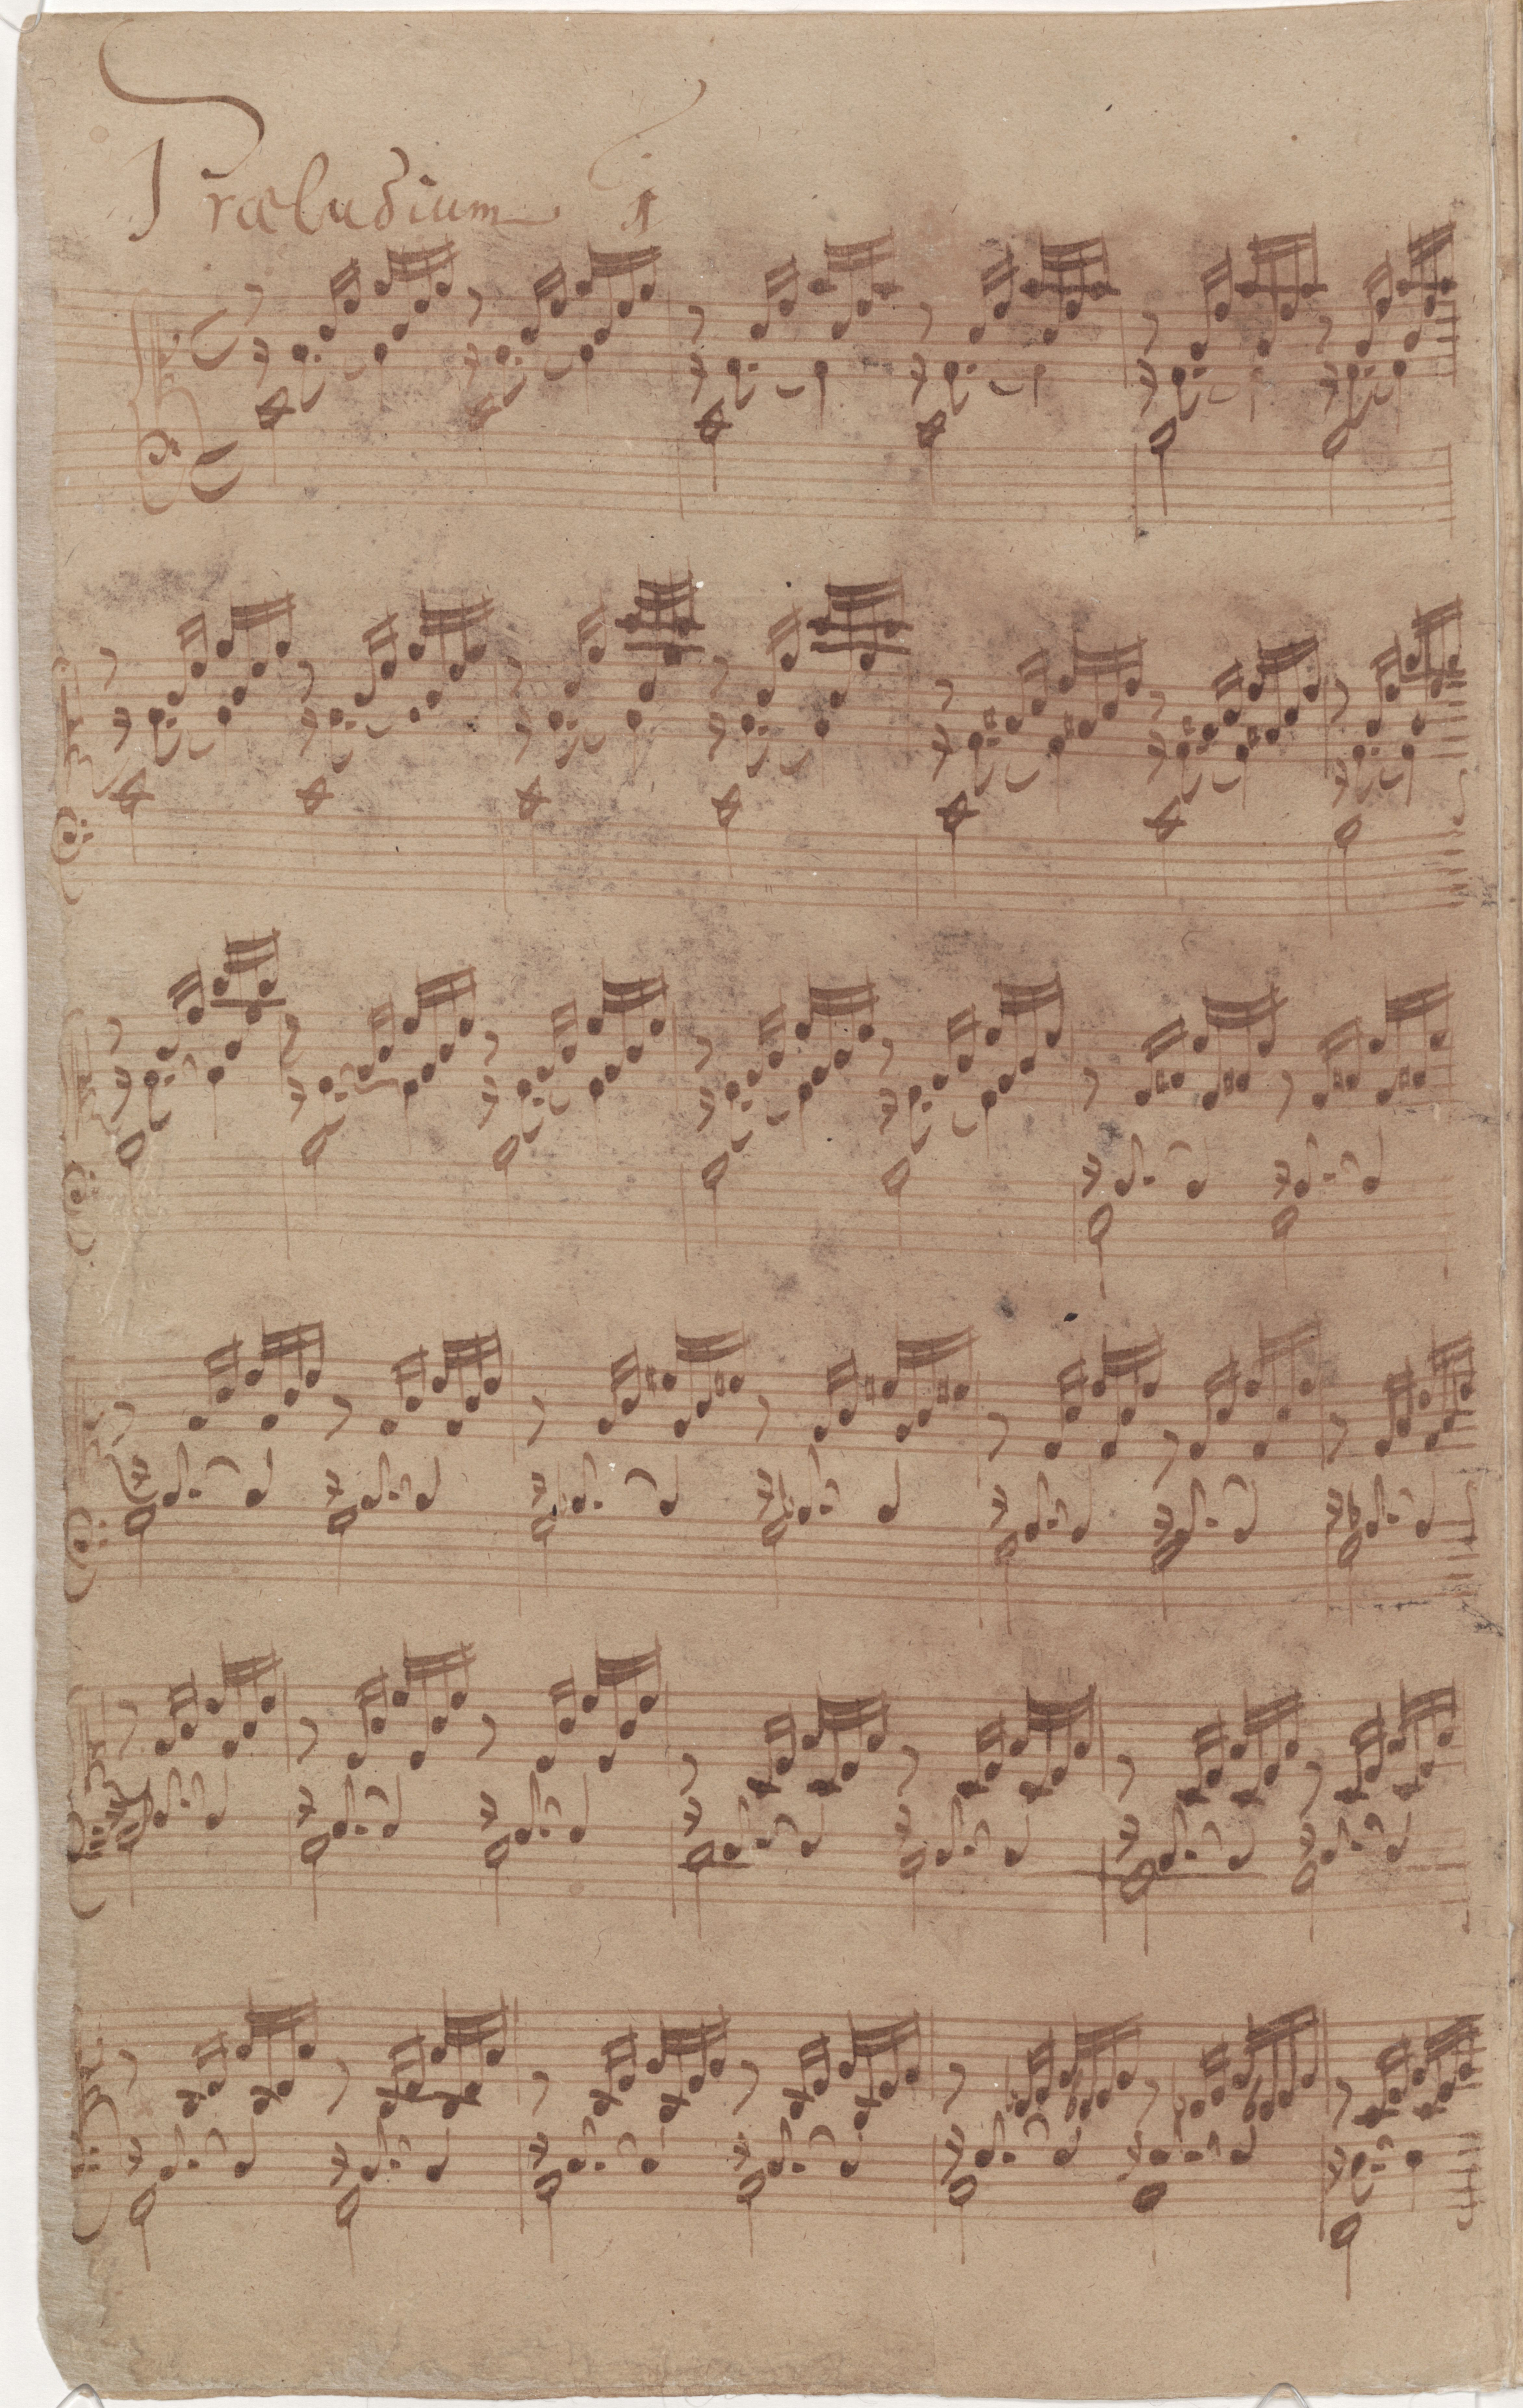
\includegraphics[height=\textheight]{Bach-wtc1-prelude1-ms.jpeg}

\clearpage

\pagestyle{plain}

\tableofcontents

% asabove.tex WITHDRAWN
% disassociation.tex WITHDRAWN
% theprompt.tex

\mainmatter

\addtocontents{toc}{\vspace{2ex}}

\preludeandfugue{The Well Tempered Typewriter}
\contributor{Sadie Philippa Kaye}

% Memory, melancholy and loss

\prelude

The \textit{Well Tempered Clavier} by J.S.~Bach, usually referred to
informally as `The 48,' is a set of two books, each book containing a
prelude and fugue in each of the 24~possible major and minor keys.  It
was written to showcase the tuning that had been recently introduced
on keyboard instruments such as organs and harpsichords, in which
every octave is divided into 12 equal intervals (semitones) and
therefore as a result the keyboard can play equally well in every
possible key. Of course, this is nowadays the usual tuning on a piano
but at the time was a major innovation.

Tuning in music makes for a fascinating topic in its own right,
combining some simple mathematics with musical harmony and good taste.

Harmony is what one gets when one plays two or more notes together at
the same time.  Two notes played together (or next to each other) are
separated by an \textit{interval} which is the ratio of the two
frequencies.  For example, an \textit{octave} is formed when one note has twice
the frequency of the other, or (equivalently) when one note has
half the frequency of the other.  Thus the ratio here is $2$ or
$1 \over 2$, depending on which you decide to take first.  Western
harmony is based originally on the intervals in a group of three notes
called a \textit{triad} built over a single note, which you can call $1$, with intervals
defined by the numbers ${5\over 4}$ and ${3\over 2}$.  One can argue that
the reason this sounds `harmonious' is that these are particularly
simple fractions.  Furthermore, if one attempted to play a note on a
stringed instrument such as a violin it is almost certain, because of the physics of the
way a string vibrates, that as well as the lowest
note (called the \textit{fundamental}) one would necessarily also play notes
(called \textit{harmonics}) at intervals $2, 3, 4, 5,\ldots$ above
this fundamental.  (Some people claim they can actually hear these
harmonics.)  The triad is nothing other than certain of these harmonics
one or two octaves lower.

Music is not static.  It has a `home' which is where it starts but it
likes to move on to somewhere else and then return. Melody is
almost always written in this way, starting `home' and then venturing
out to eventually return.  Apart from octaves, the note with the strongest relationship to
the fundamental is the one with ratio $3\over 2$ and this is called
the \textit{dominant} or \textit{fifth}.  (In this context, the
fundamental is usually called the \textit{tonic}.)  The dominant
is often the first destination as one travels away from home. By multiplication
of fractions, we can build a triad over this dominant and the new
triad's notes will have the ratios ${3\over 2}, {15\over 8}, {9\over 4}$
to the tonic, or (dropping an octave on the last of these to fit
the resulting note in the space between $1$ and $2$) ${3\over 2},
{15\over 8}, {9\over 8}$.  We can also build the triad `under' the
octave note at $2$ by \textit{division} of fractions, as
${4 \over 3}, {5\over 3}, 2$,
so that the new note at ratio $4\over 3$ to the tonic, called
the \textit{sub-dominant} or \textit{fourth}, is the one which has our
octave note $2$ being its dominant or fifth.  Not surprisingly, the
sub-dominant is another common destination.

Putting this together, we have eight notes that bear close harmonic
relationships to the tonic:
\[
1, {9\over 8}, {5\over 4}, {4\over 3}, {3\over 2}, {5\over 3}, {15\over 8}, 2.
\]
This is the well-known \textit{major scale} expressed mathematically.

An alternative scale is sometimes used\=called the \textit{minor scale}\=which
is built in the same way starting with the \textit{minor triad} of
$1, {6\over 5}, {3\over 2}$, giving
\[
1, {9\over 8}, {6\over 5}, {4\over 3}, {3\over 2}, {8\over 5}, {9\over 5}, 2.
\]

It is natural to continue this process: building scales over any of
the notes we have made so far.  There are two problems, the first less
serious than the second.

The lesser problem is that the interval between $1$ and ${9\over 8}$
and the interval between ${4\over 3}$ and ${3\over 2}$ are both larger than
any of the other intervals between neighbouring notes
constructed so far.  In fact these gaps are approximately twice as large, and
so it is natural to insert new notes to fill these gaps.  (If the
tonic were C then these two new notes we add would be C\sh\ and F\sh.)  This
done, all our small intervals between neighbouring notes
are\=amazingly!\=almost exactly the same.  This small interval is
called a \textit{semitone} and there are twelve semitones in an
octave.  The fact that these semitones are almost exactly the same is
quite miraculous and unexpected and means all sorts of music is
suddenly possible, such as playing scales in the `home' key and then
playing scales in other keys.  But, as good as this is, these semitones
are not in fact \textit{exactly} the same and repeated mathematical
tricks such as we have been playing will result in larger and larger errors.

This is the serious problem I hinted at.  It is not possible to
arrange a musical keyboard that plays perfectly in the key of C, and
then equally well in all other possible keys.  If a keyboard is tuned
to play perfectly in C, then the key of F\sh\ will certainly sound
wrong\=and many other keys too, no doubt.

Several possible solutions to this problem were known even in Bach's
day.  One is to re-tune an instrument for each piece you are proposing
to play. But this is impractical.  Another is to only perform on an instrument
where the tuning is infinitely variable, such as a violin or a
trombone, and then the problem does not arise.  Indeed many musicians
who do perform on these instruments often do so according to the `natural' intervals I
have just described\=but this solution is not available to the
keyboard player.  The solution that was discovered in the 18th century
was to tune the keyboard differently so that it could play very good
approximations in all of these keys\=but at the same time cannot
play \textit{any} of these keys exactly.  And the way to do this is to
build the keyboard so that there are twelve semitones in the octave
in which these semitones are all \textit{exactly} the same\=not just approximately
the same.

Mathematically, this means the notes in the octave
would be at the following intervals to the tonic.
\[\begin{array}{cc}
\hskip -1em
2^{0/12} = 1,
2^{1/12},
2^{2/12},
2^{3/12},
2^{4/12},
2^{5/12},
2^{6/12},\\
\qquad
2^{7/12},
2^{8/12},
2^{9/12},
2^{10/12},
2^{11/12},
2^{12/12}=2
\end{array}
\]
so that the interval between any two neighbouring tones (i.e.~a semitone) is $2^{1/12}$ or
1.05946\ldots\ 
A keyboard instrument tuned to these fractional powers of 2 is said to be
tuned to \textit{equal temperament}, or is \textit{well tempered}.

None of the notes on the new scale is exactly equal to the fractions
we discovered earlier, but for most intents and purposes they are very
good approximations and quite good enough. Most people will not hear
the difference without specialist training. In the key of C major,
the least accurate note will perhaps be B$\natural$, the
so-called \textit{leading note}, and tunes that feature this note
extensively (such as the Christmas carol, `The First Nowell') will
certainly sound different played on a keyboard compared to how it might be played in a natural
scale.  But whether it is because we are now so used to equal temperament
or because these approximations are deemed accurate enough, this
is hardly ever mentioned as a problem.

Equal temperament was a major innovation in music in the days of
J.S.~Bach who celebrated the new possibilities that this tuning gave
by writing \textit{The Well Tempered Clavier}, a set of two books,
each book containing a prelude and fugue in each of the 24~possible
major and minor keys, written to showcase this remarkable new tuning.
Under the natural tuning, this would not have been possible.

\fugue

I once attended a talk by the poet Craig Raine on his libretto to the
opera \textit{The Electrification of the Soviet Union} (music by Nigel
Osbourne, stage direction by Peter Sellars, libretto published by
Faber and Faber in 1986).  Raine had been approached by Osbourne to
write a libretto based on Pasternak's novella \textit{The Last
Summer}, this being chosen by Osbourne because it was (in Osbourne's
words) `The most musical book he knew.'  Raine was completely taken
off-guard by this.  He did not at the time, nor later when he was
giving the talk on his completed libretto, know what Osbourne had
meant.  To me, the musicality of \textit{The Last Summer} shines
through and is one of the main delights of this work, yet an excellent
poet such as Raine, who surely has some well-developed concept of
music, did not see it at all.

This is not an isolated occurrence. T.S.~Eliot wrote a well-known
essay entitled \textit{The Music of Poetry}\footnote{In: On Poetry and
Poets, Faber and Faber 1957.}, in which he never explains what he
means by `music' in poetry.  The closest he gets to a definition seems
to be the highly circular,
\begin{quote}
\ldots a `musical poem' is a poem which has a musical pattern
of sound and a musical pattern of the secondary meanings of the words
which compose it, and that these two patterns are indissoluble and
one.
\end{quote}

Thus we learn of Eliot's opinion (which I wholeheartedly agree with)
that the `music' of poetry is more than the rhymes, assonances or
alliteration that may be there and certainly more than the rhythms of
feet and metre which we hear.  Meaning plays an essential role too.
But nowhere in this essay does Eliot explain what he means by `music,'
except by appealing to the reader's preconceived idea of what is meant
by music \textit{qua} music.

We get a bit closer to what Osbourne was driving at a little later
when Eliot writes that `a play of Shakespeare is a very complex
musical structure.'  In other words, the musicality of a piece of
literature of whatever length is an attribute that incorporates its
entirety and overall structure.  These are further hints that the
music of poetry or literature is not about rhyme or alliteration or
metre but something more, perhaps something that introduces, develops
and concludes a theme in the way musical form does.  Music that really
is music must attempt to be more than a catchy ditty or mere tuneful
phrase.  In this respect, Pasternak's novella \textit{The Last Summer}
is highly musical, at least in my opinion as well as Osbourne's.

In Eliot's very last paragraph, where perhaps a summing-up is
expected, he introduces new ideas for his essay that hint at possible
future developments of his thesis that align closely to what has been
said about musicality involving the entirety of a piece.
\begin{quote}
I think that a poet may gain much from the study of music: how much
technical knowledge of musical form is desirable I do not know, for I
have not that technical knowledge myself.
\end{quote}
and
\begin{quote}
The use of recurrent themes is as natural to poetry as to music.
There are possibilities for verse which bear some analogy to the
development of a theme by different groups of instruments; there are
possibilities of transitions in a poem comparable to the different
movements of a symphony or a quartet; there are possibilities of
contrapuntal arrangement of subject-matter.  [\ldots] More than this I
cannot say, but must leave the matter here to those who have had a
musical education.
\end{quote}

I have also, for some time, thought that a closer connection between
literature and music would be beneficial to both.  One clear
suggestion for `thinking musically' in literature is to use repetition
or near repetition.  There is a wonderful use of a near-verbatim
repeat near the beginning of \textit{A Portrait of the Artist as a
Young Man} when Joyce recalls a particularly horrible prank played on
him by another schoolboy. \textit{Ulysses} abounds with other examples,
such as the \textit{Sirens} episode which is not only very much about music but
is appropriately written as if it is a movement of a symphony.

Other suggestions for music in literature involve form.  Ternary form
(with similar or related outer sections and a contrasting middle
section) is as natural for literature as it is for music; the same applies to a form like
an arch, well-loved by B\'ela Bart\'ok for example, that moves out from the initial
material through one or more other sections to some remote or
emotional middle section and then returning symmetrically back to the
beginning through the material previously traversed.

Bach's \textit{Well Tempered Clavier} suggests something else again.
This is a showpiece of composition that shows how the new tuning
successfully works in all of the 24~keys.  Bach moves up the keyboard
chromatically, alternating major and minor with a prelude and fugue in each key.
This idea of using all the
keys with an individual piece in each (but sometime with a different
ordering of the keys) has frequently been copied, for example
by Chopin in his \textit{Preludes}.
Book One of The 48 was completed in 1722 and Book Two was
written about 20 years later. It is not specified what instrument it
is `for' but would no doubt have been most frequently played on the
harpsichord.  Nowadays it is more commonly played on the piano.

(My copy of Book One of the forty eight is a nineteenth century
publication by Peters of Leipzig, edited by Carl Czerny (1791--1857)
and Friedrich August Roitzsch (1805--1889).  It is signed `M H Roberts
1889' by Mabel Helen Roberts, the sister of my mother's maternal
grandmother and was a gift to my mother from her great~aunt in 1943.
I do not remember my mother playing from this volume but she certainly
encouraged me to play these works when I was a teenager, which I did with
much enjoyment and many struggles.)

\textit{The Well Tempered Clavier} achieves much more than
a proof of concept showing the keyboard can play all these keys.
Each key invites the composer to write in a different style, always
within the constraints of an introductory prelude followed by a
contrapuntal fugue.

There is no set form for the prelude: it may be fast or slow, sad or
happy, and Bach includes toccatas, a sarabande and an overture in the
French style in the preludes here, to mention just a few.
The very first prelude, in C major in book one, is by far the best
known from the set. (Bach's autograph of this prelude is shown in the
frontspiece and cover of the book you are currently holding, courtesy of Wikipedia.)
In fact, even people who do not think they know
this music will recognise it readily. It is deceptively
straightforward music.  It can be analysed as being simply a sequence
of 35 broken chords, starting and finishing in C major (of course) but
with delightful harmonic twists throughout.  It is easy to play\=by
far the easiest item in the set\=and is frequently played by beginners
to the piano.  As well as its position as the opener of this set, it
has been used many times since.  It was used by Charles Gounod as the
harmony of a setting of \textit{Ave Maria} and has been used in a
similar way by Arvo Pärt in his \textit{Credo}.  It is used
in \textit{Repent Walpurgis} by Procul Harem; and, perhaps best known
of all, Gounod's \textit{Ave Maria} (including all the material from
Bach's prelude) was used by Andrew Lloyd Webber as the foundation to
the song \textit{Don't Cry For Me Argentina}.

The word `fugue' literally means `flight' and by Bach's day referred
to a well understood and developed musical form with typically 3,4 or
5 voices, each at a different range of the instrument, all opening with the
same main theme one after the other in the beginning section with a similar
device used in several places elsewhere, especially at the end.
Fugues have been written in literature too.  Douglas Hofstadter wrote
a Prelude and Fugue for four voices, \textit{Prelude\ldots\ Ant Fugue},
in his book \textit{Gödel, Escher, Bach: An Eternal Golden Braid} (Basic
Books 1979).  Hofstadter's work is highly entertaining and full of
jokes and puns, some of them excellent, and mimics the form of a fugue very well
through the various entries in the four voices.  It also mimics other musical
devices typically found in fugues, such as stretto and a tonic pedal.
His object is, however, didactic through entertainment, rather than literature
\textit{per se}.  Yet it always seems
to me that music has much more to offer literature, and Hofstadter
clearly had similar thoughts.  We can profitably study music for
ideas in literature.

The main feature of \textit{The Well Tempered Clavier}
that I would like to emphasise is the use of all 24~keys.  Each key
invites the composer to write in a different style or mood,
in this case always within the constraints of an introductory prelude
followed by a contrapuntal fugue.  This key or mood is exactly
what unites the prelude with the fugue.  On the surface, these
two parts of a work are not connected: one might be slow and the
other fast; one might be formal and the other free.  The key
itself makes the connection and shows how the two halves unite
to form something greater.

Furthermore, as well as keys suggesting mood or emotion, composers,
performers and those listening to music have learnt to associate
particular moods or emotions with each key.  For example, the key of
C~major is `simple' and `ordinary'.  (To what extent it is also
`plain' depends on its treatment.  Bach's C major is not plain, although
it is much more familiar and closer to home than, say, the rarified air
that is breathed in his F\sh\ major prelude and fugue in Book One.)
Similarly, E\fl\ major is often associated with the `heroic', as used for example
in Beethoven's \textit{Eroica} symphony or Strauss's tone
poem \textit{Ein Heldenleben}.\footnote{See the appendix for a more
detailed list. It is of course somewhat na\"{\i}ve to associate a
simple list of moods to musical keys: the mood very much depends on
the composer's treatment of the music too, such as whether it is fast
or slow or a dance or a song, etc.}

Whether these moods associated with keys is an innate part of our
psychological make-up or a synthetic product of the way composers have
historically chosen to write music is a moot point, but there is no
doubt that pieces of music in different keys sound very different in
terms of mood and emotion, and this can easily be verified by playing
the same music transposed from one key to another, listening to the
differences.

The same applies to literature.  If anything can convey emotion and
mood, literature surely can, and there are considerably more traits
available to the author or poet than the 24~keys available to Bach.  A
literary `key' could reasonably mean a mood, described perhaps by a
set of three or four adjectives, and `writing in that key' would then
mean writing about something that represents or encapsulates that
mood.  To keep things simple, one's writing might focus on a single
subject, though in music as well as in literature `modulations' of the
central key or mood are frequent and, for example, the much-used
musical form called \textit{sonata form} is based on contrasting two
themes initially presented in different keys, to be developed and then
finally\=as a kind of resolution\=presented at the end in the same key.

With all this in mind, this volume is a set of 24~preludes and
fugues in literature and this essay is its introductory item\=the
inital piece in the straightforward key of C~major
that welcomes the reader to the world of these~24. Each author
has been asked to focus on particular moods, emotions or traits and to
write about a person, object or place that conveys them.  Modulations
(contrasting emotions) were not discouraged and indeed Bach's~48~contain
many modulations too, but the focus is on one primary
subject.  For the chosen subject that exemplifies its moods, emotions or traits,
the authors were asked to write an
introductory `prelude' setting out the main subject in its key,
followed by a `fugue' or story or poem involving it\=which might be in
a completely different literary style.

Of course, to what extent these pieces are musical is up to the reader
to judge, but we have all found the exercise useful in finding new
ways to think about what we write.
Some authors here have taken the
idea further by experimenting with musical repetition and variation\=of key
words, phrases,  or paragraphs and concepts.
In this way we hope to expand and develop
literary style and technique in writing.  But most of all,
these pieces are to be enjoyed, as we have enjoyed writing and sharing them, and we sincerely hope you will
enjoy reading them too.

To finish, I quote from Peter Sellars in his `Director's Note' for the
opera, \textit{The Electrification of the Soviet Union}: `There is not
really a plot in this opera, although there may be an argument.'  The
same is true of this book, and perhaps it is also true of all great music.  Sellars goes on to quote Pasternak
himself, recalling a paper he presented to a society of young artists
saying that, `My paper was based on the idea that our perceptions are
subjective, on the fact that the sounds and colours we perceive in
nature correspond to something else, namely to the objective
vibrations of the sound and light waves.'  Perhaps you, dear reader,
will see something extra, something different, in the juxtapositions
brought about by thinking musically and writing in a particular key.
But at this point I shall stop.  For I observe that, here in this essay, where
you were most likely expecting a well thought-out and clearly expressed summing-up, you
are instead being bombarded with yet more ideas from me, and ill-thought
through ideas at that.  T.S.~Eliot would surely approve.


\preludeandfugue{Death of a Piano}
\contributor{Brynneth Nimue Brown}

% Memory, melancholy and loss

\prelude

Modern pianos have steel frames to prevent the wood from warping. My
grandmother's piano survived for about a century, in spite of only
being wooden. Built for a cold home, the piano could not cope with
central heating and, in its final years, became untunable. No matter
the sentimental value, a century-old piano is too large a thing to
keep when it can no longer be played. The memory of it lives on in me.

\fugue

I found the small, dead body on the stairs, pitiful and soggy from
having been chewed. The cat who had previously brought the little
rodent in had inevitably caught it after a few weeks of hide and
seek. I had been aware of the mouse and had surreptitiously been
putting out food and water, partly to give the mouse a fighting chance
of survival, partly in the hopes of protecting the many things a
hungry mouse might otherwise nibble.

The mouse had been living inside my grandmother's piano. I found this
out during the summer while watering the piano. We had been advised by
a tuner that a pot of water inside the body would help prevent the
wood from drying out in hotter weather. I duly took responsibility for
piano watering. When I removed the dark board from above the pedals, I
found a little stash of dried pea flakes: food I had put out for the
mouse had been stashed here, in a furtive, hopeful way.

I wondered how often the mouse had been inside the piano while I was
playing. What sense could it possibly have made of the sound? I
worried that I might have frightened it. At the same time, I hoped
that it had somehow been able to appreciate the music as much as I
did.

The piano came into the house when my grandmother was a child. It
brought sorrow in the form of an abusive music teacher, but it must
also have brought solace. She kept it for most of her life and
persisted in playing it until her hands could no longer manage the
keys. Whatever it had cost her, she evidently considered it worth the
price. The piano outlived her marriage, and her parents, enduring to
watch over my childhood and to accept new small fingers on the
keys. It came with stories of wilder times, parties and musicians. I
grew up with the music she chose; classical pieces played with more
passion than skill, and a relentless determination to improve.

She did not really play for other people; the music held a private
place in her life. If she had ever aspired to be professional, she
never mentioned it. She was always the hobbyist where her brother was
the professional. This held true in both music and art, where he had a
career and some side hustles, and she had her quiet dedication.

I do not know what she dreamed of, or where her mind went when her
fingers were on the keys. She held no ambition on my behalf, never
spoke of success or achievement. She simply wanted me to play, and
there was a gift in that, which offered possibility, while making no
demands.

In old age, a stroke robbed her of the use of her left hand. She
fought to regain motor control, fought relentlessly to claw back what
had been taken from her. She played, badly and persistently, ringing
defiant notes with a left hand no longer able to keep up. There were
difficult pieces she eventually abandoned but sheer bloody-mindedness
brought some material back under her fingers. She refused defeat.

When she could no longer play, she insisted that I must have the
piano. She wanted my small son to learn. For some years, the piano sat
in my front room, exiled from its home, and a little lost. There is a
stoicism in pianos. I could not bear to think about how that other
room would be without it. A room that for my entire life had existed
only for piano music. Emptiness is more than a question of unfilled
space; death can seem like an event, but it is more normally a
process.

No doubt the mouse who lived in the piano died quickly, but the
process of that death began weeks previously, in capture. A piano dies
slowly as time takes a toll on the structure of wood. Dreams are also
slow to die. Hope fades in a life that is not lived fully. The piano
stands untouched, accumulating dust. Marriages die in small doses of
everyday poison, in carelessness and casual cruelty. Homes are
abandoned, envisaged futures melt away, leaving only stains and
regrets. Sometimes it is a kindness when memory fades.

After my grandmother's death\=after the death of her piano.

I remember the dark green cover of the preludes and fugues. I did not
choose them but had them thrust upon me by a teacher who had no
interest in my preferences. There are many ways to kill a dream. I
have no memory of specific notes on the stave, only the density of it
and my own annoyance. Like my grandmother before me, I played with
more passion than skill and Bach did not agree with me. I remember
frustration, the death of joy in my own inability to make this music
come alive under my hands. I can still remember the feeling of those
old keys beneath my fingers. The one with a horizontal crack. The
round hole that looked like a cigarette burn but almost certainly
wasn't. Cold keys on a winter's day. The subtle difference of texture
between the white and the black. Some tunes remain alive in my
head. Chord shapes and runs of notes live on in tactile memory.

The piano is long gone, but when I type, I remember the lessons
learned from other keys, writing with more passion than precision,
words that my fingers find as though they were still trying to release
the clear notes of long dead composers.
% prose
\preludeandfugue{(No) Lingua Franca}
\contributor{Irena Peterson Pavliuk}

\settowidth{\versewidth}{Oh, throw me into the dark deep water\=it knows us so well.}

\prelude

\begin{verse}[\versewidth]
  
Oh, leave us without your curiosity.\\
The colonial tongue is no lingua franca for us.\\!

We are not even the children of the murdered ones.\\
We are the children of those who kept silent\\
and, thus, survived.\\!

My mother lives in deep countryside,\\
from where her voice is not heard.\\
My father talks to me about politics from the clouds,\\
he did not live to see the revolution.\\!

I am the child of those who kept silent.\\
Chances are, you are as well.\\
Is this why you are all so quiet,\\
and I barely know you,\\
but also have known you for lifetimes?\\!

\end{verse}

\fugue

\begin{verse}[\versewidth]

Songs of the forests\\
\qquad we share,\\
flapping of the wings over the fields\\
\qquad we share,\\
dark seas where we feel at home but with so much pain\=\\
because what is home and for how long?\\!

We share\\
\qquad the habit of being quiet,\\
we share\\
\qquad the custom of saving bread.\\! %was:  for tomorrow.\\!

We share\\
\qquad being seen as those behind the wall,\\
we share\\
\qquad being not seen at all.\\!

\vspace*{1cm}
%\[-\]
%\textbf{3}\\!

Emergency backpacks\\
in the cellars \\
of our homes\=\\
we're not burdened with the material things\=\\
it's called minimalism;\\
it's now in fashion.\\!

We play games in the woods;\\
we jump over fires on Midsummer's Eves;\\
we jump over fires\=always!\\!

We played games in the woods:\\
I learnt to make a perfect dugout when I was five\=\\
my grandpa didn’t like it.\\!

\clearpage
%\[-\]
%\textbf{4}\\!

The remnants of self-preserving:\\
they read it as nationalism.\\
I read it as `try to shame me'.\\!

Oh, take me to my Midsummer's fire and try to shame me.\\!

Oh, throw me into the dark deep water\=it knows us so well.\\!

The sweetest song my grandmother sang.\\
The sweetest song your grandmother sang.\\!

The water does not speak the colonial tongue,\\
but it knows our songs too well\\
and needs no lingua franca.\\!

\end{verse}
% poetry
\preludeandfugue{Piper Finchling}
\contributor{Steven C.~Davis}

\prelude

Piper\=was. She was\=what? She fluttered her wings and cheeped
inquisitively. She was.

She fluttered her wings again, rising off the ground a little way. She
was in a forest and sunlight was slanting through the trees. The air
smelt of earth and acorns and optimism\=she trilled excitedly, turning
too fast and nearly falling, confusing her wings with her hands for a
moment before regaining her balance.

There was a path running through the trees. The trees were not thickly
spaced but they did grow tall. She tilted her head back and back until
she was tumbling downwards again and squawked in distress, in
surprise, gaining the ground without harm. She looked up again. Sat
down. Lay down, so she could properly see the sky.

It was blue and gorgeous, with brown-limbed trees and branches
caressing it, with leaves in all shades of hues intermingling with it,
until she wasn’t sure where tree ended and sky began.

She chirped in delight.

Cheeped.

Squawked.

`I wonder\='

She chirruped softly. There were sounds, and they were her.

`I can speak!' she chirped, turning her head this way and that to see
if anyone had heard her, if there was anyone else nearby.

There wasn't, but that didn't mean\=

`I can talk!' she cheeped delightedly.

\fugue

Part golden, sepia light spilled through the forest.

What she had taken first\=upon becoming\=as trees, Piper realised now
were so much more. They grew out of the ground, in the shape of trees,
but the lower trunk and branches were bookcases and shelves and
contained within them were tales, written on leaves and bark, scrolls
and parchment and books themselves, printed from pulped paper, but
everywhere, books were part of the trees.

The air smelled of acorns and parchment and as she fluttered closer to
an old oak, she saw he had bookcases all around his trunk. The books
within were brightly coloured in the colours of autumn, reds and
yellows, browns and dusky blues, the text in black, like veins or the
capillaries of a leaf, edged in gold.

Piper lifted one experimentally. The tree stirred, shedding a pair of
leaves that slowly spiralled downwards, as if acknowledging her
opening the book.

The skin of the book was bark, rough against her hands. She fluttered
her wings excitedly, closing her eyes and tilting her head back,
splaying her fingers across a page. The page felt like a leaf, brittle
and ephemeral, fragile, but containing so much.

She whistled wordlessly.

The next book was a scroll, an unwrapping of bark, but a bark that
crackled and creaked like an old oak, caught in a storm. The letters
were etched in black, but lined with gold: the colour of autumnal
nights.

Piper whistled. The lettering was lovely.

She ran a fingertip along the curls and slants. The shapes defined:
she didn't know what they all meant, but there was beauty in them and
beauty in the not-knowing.

She wrapped it up again carefully and returned it to its place on the shelf.

She fluttered back down to the ground. There were leaves scattered all
around: golden and red and brown, pale green and dark yellow.

She gave a half-cheep of delight and flung herself down, extending her
legs and her wings this way and that before jumping back into the air.

`I'm an autumn-leaf-angel,' she chirped, flapping her wings excitedly,
watching the leaves scatter and wash over each other, watching them
stir and move as if dancing, as if pulled by invisible strings.

A gentle breeze blew.

She flew into it, feeling the wind pass between her feathers, feeling
the wind move around her, feeling it lean into her, forcing her to
flap harder.

She spiralled down around a weeping willow, the air cooler, stiller,
the wind less noticeable. The grass was greener, deeper, softer, with
patches of moss and tendrils of willow wisping gently in the breeze or
by its own accord.

She touched down gently, shaking her wings. The ground was softer and
the air was damper, smelling of earth and mud and water. She walked
around, looking this way and that, looking for the stream, listening
intently for the sound of water tinkling across rocks, but there was
no sound of water, only the presence of water. %SPK

There were few leaves around the willow. No second go at being a
leaf-angel, and she thought the dampness of the grass and the moss
might get into her wings. Piper fluttered her wings.

There were no books in this part of the forest either. The willow tree
was a willow tree.

She fluttered up again. The wind had eased down, and though, carrying
on in the direction she had started, the trees grew together thicker,
there was also a more intense golden light spilling through the high
branches and the leaves, cascading down in slanting beams of yellow
and orange and red. Here, leaves spiralled down blissfully, coasting
between the trees, as if a gentle breeze carried them safely to the
ground.

She fluttered towards the light. There was a misty, ghostly, soft feel
to it, as if the sunlight were being streamed through fog.

As the trees neared, she saw that instead of shelves with books, as
previous trees had been, these trees had smaller doorways set within
them, each containing a single book. She fluttered up to one, staring
in surprise. %SPK

\textit{The Adventure of Time}, she read, looking around wildly.

She was alone in the book-forest, as far as she could see.

No one else was around to have spoken.

`I\=' she stared at the book-within-the-tree. `I can read words?'

She could read the author's name. She opened the cover with her wingtip,
and words jumped out at her in a tangle of consonants and vowels. The
letters were tighter and smaller than the previous book she had looked
at, and\=there was something a little depressing about them, Piper
felt.

In the other book, with its black and gold lettering, the letters were
free and rounded and swirled this way and that in beautiful
curves. The words in this book all stood in a line,
shoulder-to-shoulder, as if rounded up and corralled to not stand out
from one another: to present a united front.

She squawked disconsolately.

`I can read letters,' she cheeped softly. `But they look trapped and
lined up.'

She moved another page on, turning the crisp, cream, parchment with
her wingtip. The words were more broken up, following. They still had
a uniform, hard edge, but there were lines that weren't full of words
and could breathe, and there were gaps between paragraphs and stars,
as if the author wanted to draw the reader's attention away from the
text to another place.

Piper cheeped, a little happier.

She closed the book and flapped over to another tree. This tree was
broader, thicker, and the doorways were larger, the books within
larger, and there were even little seats in front of the books.

She opened the book carefully. For such a large, impressive tree, with
grey-brown bark faintly glowing in a soft-golden light, the book cover
was pale blue, the blue of a sunrise, not quite evolved, but caught
and reflected across water, splashed through with curls of golden
light.

She trilled with delight. The words were larger, given free rein
within the page, and there were bright images accompanying the
text. The words' meaning was just there: a tale for a child, for one
young and curious, of delightful things to explore and find.

She turned the page.

The tale continued and now she could read the words without needing to
run the edge of her wingtip across the curls and curlicues. The story
was\=she tweeted excitedly. She didn't have to think about it! The
tale was forming in her mind as her eyes beheld the lettering.  She
cheeped excitedly, closing her eyes and leaning back a little.

Wisps of sunlight warmed her wings.

Piper launched backwards off the tree, spinning in the air for a
moment, the sunlight catching and warming her wings. She carried on
spinning backwards, enjoying the feel of being slightly out of
control, of being warmed by the sun, of being surrounded by\=words and
tales and stories that she could read!

She cheeped, regaining her balance. There were tall trees all around
her, each offering a plethora of books to read, some large and
beautifully colourful, others densely and tightly packed with uniform
letters.

`I can read anything I want!'

Piper fluttered forwards. There are enough books here, she thought, I
can spend the rest of my life reading and\=a little cross-breeze
distracted her and she quarter-turned, surprised, and saw that to the
left of her, the book-forest extended, but the golden light bled down
to a foggy-white light, though the space between the trees was still
bright and intriguing.

She allowed the breeze to carry her towards the foggy light.

The trees were very similar, though smaller. The air was cooler,
crisper, sharper almost. It wasn't cold, as she'd expected, the light
seemed clearer though less warm in colour.  `How big is this
book-forest?'

She fluttered into the crisper, foggy-white light. The trees had more,
smaller, branches, and at the end of each small branch was a door,
smaller than the ones in the golden-lighted forest, but still each
held a book, the doors all open so that she could peruse.

She fluttered across to the nearest one. The light was softer,
gentler. The book was about a journey, she realised, though it was a
large book and the text was crammed in very tight. She could smell
excitement and pain from the book; swathes of scenic description and
human endurance.

She wriggled her beak a little. It was a very big book. It would take
me a very long time to read that, she thought.
% OR: It would take her a very long time to read that.

She fluttered over to another branch and another door.

The book tasted of courage and confidence. There were pastel images
and a mixture of solid text, though in much smaller groupings, and
curved text to go with the images.

She opened the book further, scenting a tale of friendship, of
overcoming adversity.

Can others do this?~she wondered. Do they have to read all the text or
can they tell what the story is about from a page or two?

She closed her eyes. The book was lovely and she could feel the warmth
from it, a little brighter than the foggy sunlight that cloaked the
trees.

The warmth seeped into her.

Should I go back to the start and read the books in order?

Should I continue randomly flying from tree to tree and seeing what
books the trees have to offer me?

Her breathing slowed. The tree was breathing; she could feel it. Soaking
in sunlight. Drawing in moisture from the earth it was buried deep
in. Patterns of communication ran between the trees, unseen,
unheard. This could be my home, she thought. I could stay here and
there would always be something new to read, and warm places to sleep,
and sunlight and rain, occasionally, if the temperature became too
hot\=or maybe I would move next to the willow for a while, where it
was warmer and damper, where the ground was softer.

I could stay here, and never see what else there is to discover.

She frowned, in her almost-asleep mode. I want to see what's out there.

I like the forest, but there is so much more. And I can read now.

She shifted her footing, waking herself up.

The ground was warm. The branch was warm. The light was soft and
muted. She could fall asleep anywhere and knew she wouldn't fall to
the ground: and even if she did, the ground and the trees and the
books would catch her and she would be safe.

Piper squawked, looking around.

In the distance, she could see the edge of the golden-lighted
trees. That way was beautiful, both the trees and the air and also the
books. But I've been that way.

She looked around. Further away, but pushing on in the same general
sort of direction, the foggy-white light seemed to deepen to a
strangely blue-tinged light.

She launched herself off the branch, chirping inquisitively. The foggy
light swirled around her, windless, but didn't hinder her as she set
off for the strangely hued blue light.

It came nearer and nearer and with it came the scent of salt spray,
and strange, splintering, crashing sounds.

Are trees falling?~she thought, in trepidation and horror. I don't want
to go where trees are being destroyed.

The serene blue light grew stronger. The trees thinned out and more
light spilled between the gaps.

And there was a golden glow as well, though it seemed to rise from the
forest floor. And ahead, beyond the trees, the blue grew stronger and
wilder.

Trees thinned. The ground became rocky, then salty, then sandy, and
then Piper was beyond the trees\=waves battered on a sandy
shore. Sunlight sparkled on the waves and the sand and the sea horses,
curling and crisping, crashing against the rocks and being dragged
back out and then rising, riding again at the shore, crashing and
dissipating and reforming.

There were no books: there were no trees for them to be hosted in. But
the sunlight sparkled in rainbows on the deep blue of the ocean. The
air was salty and tangy and sharp, and carried the scent of water, a
coldness she'd not felt in the forest.

She fluttered down to a sharp boulder, jutting steeply out of the
golden, stony, sand.

The sun warmed her wings.

Far, far beyond the curling and crashing waves of blue there was
another land, low on the horizon, but visible.

To the north, the beach continued, skirting the edge of the forest
until it became lost in the sandy blue of the horizon.

To the south, though that felt like turning back to where she had come
from, the beach continued unbroken until it met the sky.

Piper fluttered her wings excitedly. There was a new land, out there,
beyond the golden-stroked ocean, beyond the deep waves of blue.

Can I fly that far? Is there somewhere to rest if I am halfway across
and my wings grow tired?

She turned to look back at the forest, stretching out behind her.

`I liked the book-forest. I could have spent my life there, happily,
if I was someone else.'

She turned back to the ocean and the crashing waves, the rocks that
glistened with seaweed and salt, that gleamed, polished bright by the
waves.

And the land beyond that, low on the horizon, though she could see
peaks and ridges, drops and swells, as if the edge of the land were a
mountain.

I can fly up mountains, she thought.

I can fly across an ocean.

I can explore.

Piper took to the wing, beating out across the ocean.


% prose
\preludeandfugue{The Border, or `Offa's Dyke Brought Back up to Serious State-of-the-art Spec'}
\contributor{Richard Bruce Clay}

(The Scene: The Anglo-Welsh border, close to Hay-on-Wye, a few years
from now, in a version of the world that seems pretty close, but not
quite the same as the one in which we live.  A guard house, well
protected by a couple of machine gun towers, stands next to the border
checkpoint.  Away to the north and to the south, the concrete wall and
the minefields of the redeveloped Offa’s Dyke stretch.  Several very
young men menace Luke and Mattie, two brothers of about thirty, who
are trying to get across into England.)

\prelude

\paragraph{Luke Irmin Ith-Cayle}\strut

A man in his twenties pointed a gun at me, so I had to take more
notice of him than I’d have preferred.  In general, I take notice of
people who point guns only because of the danger; aside from that,
such people seem only tedious and annoying.  If someone points a gun
though, I recognise the importance of setting aside things in general
and focussing on the particular.  My twin brother, Mattie, tells me I
have much greater difficulty than almost anyone else in setting aside
things in general.  He may have a point there.  He also calls me a
‘saft sod’.  He may have a point there, too.

The man pointing the gun wore a grey shirt, as people pointing guns
tend to.  % "tend to"? or "tended to then" "tended to in those days"?
A badge pinned to the shirt identified him as ‘D.O.~%
Cregsmore’.  He kept his mouth tightly shut, his lips thin.  He meant
this, I thought, to project an aura of unfriendliness and danger.
From the way his subordinates treated him, I would say he succeeded.

‘Business?’ he asked.  He kept his voice very low\=at the bottom of
the range his youth and size allowed.  Again, he intended this,
and intended it for the same reasons as he intended the facial
expression.

‘We got the stuff,’ Mattie said from over my shoulder.  ‘You know, the
papers.’

The young man with the gun looked away from me and at Mattie.  His
mouth loosened a little: to him, Mattie would seem more likely than I
to tell him the things he needed and expected to hear.  Mattie had a
talent for giving that impression\=to almost anyone.

‘Oh ar?’ said the young man.  ‘Let’s see.’

I reached for the inside pocket of my coat, pausing with my hand about
to disappear behind the collar and waiting for his nod of permission.
Reluctantly, it came.  I drew out the sealed envelope and handed it
over.

The young man holstered his gun with a slight snarl that looked
impatient.  He tore open the envelope and drew out… one, two, three
sheets of paper.  He looked bewildered at finding so many: no one
would have asked him to read so much in years.

His brow knotted in fury: he had a great difficulty in working out
what the typed letter was telling him.  I knew better than to try to
explain anything: I would appear to be patronising him and, in front
of his subordinates, that would justify his getting his gun back out
and killing both of us.

‘What’s this then?’ he snarled, looking up\=at me.

‘What bit do you mean?’ I asked, guessing what had upset him.

He waved the paper at us, thumb close to the word that had offended him.

‘University of Birmingham,’ I said, ‘at Ystalyfera.’

‘There ain’t no University of Birmingham!’ he shouted.

I did not reply.

‘There ain’t no University of Birmingham!’ he shouted again.

None of us spoke for a few moments.

Slowly, he turned to his subordinates.

‘Let them pass,’ he grudgingly grumbled, ‘but slap them about a bit
before you do.’

I felt relief and I knew Mattie would too.  The beating we could put
up with: we’d been taught well (thank you, mom) % capitals not needed IMHO
how to minimise the
injuries it would inflict.  I also felt annoyance: some clown had
failed to appreciate the inevitable result if our travel documents
mentioned that our journey had anything to do with a university.  When
people in grey shirts with guns heard the word ‘university’, you had
to expect a beating\=at least.

\fugue

\paragraph{District Overlord Harold Cregsmore}\strut

One of them is just a wanker.  He is.  You can see he is.  He just is.
The other one’s a bastard.  He is.  I can spot when someone’s a
bastard. I’m the sort of bloke who can always spot when someone’s a
bastard.  And with bastards, the thing is, you’ve always got to give
them a kicking.  That’s the important thing.  It’s your duty not to % typo?
forget that you’ve always got to give them a kicking.  A slapping is
okay, but what’s really wanted is a kicking.  Better still if % WAS The best thing is, if
you can kill them, but tonight, it’s getting late and we all want to
knock off so we’ll let them off with a slapping.  Wouldn’t be that way
usually!  Wouldn’t be that way at all!  You get these people, these
Welsh bastards, and they come over here!  They come over here!  And
they talk about ‘universities’, like we’re that sort of nation, like
England is the sort of nation that’s prepared to put up with that sort
of bollocks!  These sort of bastards are the sort of bastards who need
telling what is what!  Because everyone needs telling what is what!
That’s how it is!  Is!  Is!  Is!

Because once you say what something is, you can kill it.
% prose
\preludeandfugue{The Room}
\contributor{Irena Peterson Pavliuk}

%Confinement — Restlessness — Absorption — Irreconcilability — Legacy — Metamorphosis

% \paragraph{TITLE:} The Room (in D minor)

\prelude

This room is lined with restlessness in my body. Every time I think
about my possible return to where I come from, something small and
defenceless shrinks inside, among the apparitions of fear\=bulky and
gray. When I touch them with my finger they fall like towering
cardboard decorations that first seem insurmountable, but sway from
one concentrated and firm pressure\=then I know that deep inside I am
not at all that small and helpless. You remember, you never allowed
yourself to be small.

\fugue

I was born as a grown-up in this room. No, another room: the room next
door, which was even smaller. We moved into this one when dad asked
the dormitory concierge for a bigger and better room\=the whole twelve
square meters\=for a young family. I was my father's fourth
child. His first child remained a mystery: father did not recognise
him as his own and I trust my father’s words. The second one was also
not his own, but he loved the boy’s mother, who unfortunately died and
the boy was taken away by her relatives. And the third baby, my
half-sister, was taken away by my father's ex-wife after
divorce. Father said: you have a brother and a sister.

Regardless of age\=for example, I was a hundred years old at
birth\=we are a young family; dad doesn't tell my mother he loves her, dad
says I'm the prettiest baby he had ever seen.

At first, we live just with mom, without dad, in a tiny room that is
more like storage.  Nothing really fits there except a bed, a table,
and probably something else\=a closet? All the relatives who have
gathered to look at me as a baby are gently rustling in the corridor;
their voices are like wind; it is followed by a shriek: a piece of
wall plastering falls on someone tall, and someone hits their elbow
against the sink counter.

We started living with my dad only when I was seven months old. My
mother ran out of breastmilk, started feeding me from a bottle and put
me to sleep in a crib.

Hello, dear Room.

You are my compressed world, in which everything is skillfully stacked
one on top of the other, and other things forcefully shoved into the
chest of drawers, the door of which hangs on the insulating tape.

And if you don't get distracted, then go straight: upstairs to the
fifth floor. It’s 121 steps, but it depends how you count. Does the
last step count or not? I know all the ways of counting, I know how to
do it differently, some games involve multiplication and division, and
some involve running down and out into the street, as fast as you can!

My room envelops me in its creeping vines, and I do not know whether
it is a warm and familiar embrace, or a desire to grind my bones,
twist my body like a sheet in the wash. Within these walls, my body is
a flattened and damp towel hanging over the edge of the wash
basin. Warm hands are about to care for me, wash the towel in caustic
detergent\=oh I have so many spots\=pouring bleach on every spot;
later, under the caring and loving effect, the dirt will come out of
it, but the colour and structure of the fibres will not be restored,
instead only a whitish-blurry circle will remain. The hands will twist
it and hang it fluttering in the wind to contemplate the world from
the height of the fifth floor.

My body flutters in the wind, attached by five clothespins to the
rope. A birch twig touches the burnt circle with its earrings, a rusty
balcony railing touches the other edge. Someone lights a cigarette
next to me and I absorb all the smoke and I absorb all the phone
conversations with swear words, simple manner of talking and `witty'
profanities and I absorb the screech of a tram turning around at its
terminus and I hear the announcer say something about how this city is
the country’s most comfortable city to live in.
% prose
%%% WITHDRAWN \preludeandfugue{Disassociation}
\contributor{Dana Archer}

% Biography

% Dana is a fiction writer and film critic who is currently seeking to
% publish her debut novel. She is an avid reader and has written for
% many years in a number of formats from fan-fiction to short stories.

% This is all my own work and I hold all rights to it. It is written
% from experience and is not slanderous or misleading.

% Words chosen - Tense, Illusory, confusion, Fractured sense of reality, Disassociation 

\prelude

Disassociation is about as hard to describe as it is to spell. It is a
feeling of being somewhere physically but mentally somewhere entirely
different. Although I eventually realised that this feeling has a
name, it still perplexes me. Maladaptive daydreaming is an
increasingly common yet massively under-researched psychological
disorder where a person daydreams excessively and sometimes to a point
where reality becomes numb by comparison. Paracosm is the term used
for this other world, one that is crafted sometimes with aspects
borrowed from media and fandoms. Unfortunately a world crafted over
many years can become more a prison than an escape as it numbs the
constraints of reality with a place unburdened by logic.  It's
interesting that music is the prompt for this anthology as often it is
a key catalyst for the daydreams. It is impossible to ever fully
replicate the experience of being engulfed inside your own mind to the
point that it invokes a dissolution of reality.
% However, with this piece I aim to try and convey the feeling of
% being trapped inside a world you’ve created, a euphoria that has
% taken many years to build only to become a tomb. With it comes
% memories and moments from your life that you had spent so many years
% running from. Excessive daydreaming at its core is an escape, a
% reaction to several external factors such as Trauma or loneliness.
What really is this feeling of being trapped inside a
world you've created, a euphoria that has taken many years to build
only to become a tomb? And what memories come back? What moments from
a life that you had spent so many years running from? Excessive
daydreaming at its core is an escape, a reaction to several external
factors such as trauma or loneliness.

\fugue 

I didn't notice it at first. This was odd really, as it was just as
% perhaps the most
present then as any time later on. [This paragraph made no sense to me in the context of what comes later so I have rewritten it.]
% \marginpar{prevalent?} it had ever been.
To start with, it was just a constant trickle, a gentle drop gliding down the
glass hidden behind a curtain. Of course,
% as much as it was always there,
ignorance of its presence yields 
innocence, comfort yields longing. I struggle
to remember there ever being a time when these feelings weren't present, but there
must have been one. At some point there must have been silence too, yet I
fail to recall it.

I am sitting in a room full of my peers, yet only being able to hear
that dripping, tapping at the window. An infinitesimal sound is somehow
overpowering a room filled with voices. I once remember walking
through a crowded shopping centre during a bout of extreme heatwave;
people were rushing in all directions and I didn't notice them. They were packed like
sardines in that concrete catacomb of capitalist necessity and I was
oblivious of them. There was no dripping as the sun baked through the glass
ceiling, beads of sweat making puddles on the ground beneath us.
I was there physically, but my brain wandered, longing for the slightest
indication of rain. It traveled far that day in pursuit as I fought
through every step, desperate to stay present. But there doesn't have
to be rainfall to create condensation and the puddling heat proved an
unrelenting motivator.

I had built a world that my brain couldn't resist, an addictive tonic
to my own dismal reality.

As I aged, I became more aware. Escape doesn't serve me, nor will it
better my mental state. It might in the short term, perhaps, but not
in the long term. At first, I welcomed it, but it soon evolved into a
dangerous time-consuming crater. An addictive resort in which my mind
longed to revel in.

Around that time, the transparent teetering increased to a patter.
[I don't understand:  you've said it was just as prevant at first so how can it increase?
Since you seem sure it is increasing I changed what you wrote before.]
A tapping against the glass, concealable sometimes through music or
distraction. It never dissipated however, growing in strength,
demanding my attention. At times, when my attention was already
scattered between multiple needs, it screamed at me. Its steady
knocking evolving into a thud not unlike a demolition mission outside
my window. I wouldn't hide\=I couldn't. Although I happened to be
preoccupied, it waited silently for any brief interlude. A tempestuous
conflict with my brain and my existence. I had offered myself a
better alternative and my brain refused to part with it.

On a day I'm unable to pin-point, I allowed the droplets
in. Engulfing myself under their refreshing majesty. It was a moment
of sheer euphoria, a relief which I hoped would bring with it the
denouement to my torment.  As I stood beneath their dizzying waterfall
of oblivion, bathed in disappearing worries I little knew know what
the real world had turned its back on.

I've realized I was wrong to invite it in. What was once a patter had
become a wave. If I am lucky, I can hide away before the water
thickens. Today, however, I have found myself at the mercy of a tidal
wave. I used to run away, squeeze myself into a corner as the
rapturous aqua phenomenon washes away every aspect of life possible. I
learned quite early on that I couldn't out-run it and hiding from it
was illogical. So I simply stand, facing head on to that which has the power to
wash me into oblivion.

Oblivion wasn't so bad. [I don't understand.  By what you say in the last paragraph you haven't reached oblivion yet.]

As I allow the wave to take me, I swirl around in a
hurricane. Disorientated and lost, I try not to ponder or
guess. Navigating the numbing cold would be a waste of what little
energy I am permitted.  A limit of my own consequence. As the water
settles, I am somewhere in the middle of nowhere. This doesn't
frighten me as I look around for signs of life. [Ambiguous. Do you mean the search for signs of life
  prevents you being frightened, or that you are looking around for signs for life and simultaneously
are not frighted for a different reason?] Unafraid, I find
myself staring into the eye of a solitary hurricane resting above an
onyx underbelly. Confident that only I fell [fall?] privy to the wave, I look
down. The water splashes and shifts as I part it with my fingers. I
have no power here. Still, I squint aimlessly trying to see the
elegance embedded within the dark.

I decide to swim down.

Swimming forward would prove futile, there isn't anything to see above
the surface. [New paragraph here?] Beneath the darkening ocean is a collection of debris
and dust. Swimming further into the abyss, I find a glimmer of
light. A delicate speckle of illumination. Tiny glimmers upon the
rocks, my lungs tighten, it's becoming harder to breathe. The further
I go, the harder it is to move. I am sluggish, my muscles tighten. I
am becoming anchored to the deep.

Refusing to face defeat, I fight against the current. My body is
pleading to stop and yet I am not dissuaded. Continuing downwards. I
cannot die. It might tell me otherwise but I have grown skeptical of
the voice. Exquisite beauty has crystallized over years of
solitude. Untouched, unscathed, aged by its surroundings\=this is
new indeed.  Narrow at first, I am hunched into a crouch as I
barely make it through the small chasm.

I spare a thought for the world I have left behind. Sharp uneven walls
scrape and pull at my skin as I push past. Those who continue will
establish rules and beliefs for the many to follow. I only hope they
are kinder than before the wave. Dark algae coats the rocks, marking
my skin with lines and dusting. Perhaps I'll be a myth, a girl who
waited as the wave washed her away. A girl for whom the world wasn't
enough\=so she had to build one. A smell is developing, pebbles under
foot prove tricky to pass over.

`She never did fit anywhere,' neighbours will muse.  Perhaps they'll
write books, make documentaries\=media and culture often tries to
unpack what the public won't understand. Not that any of it matters to
me now. I became socially isolated due to fear\=a fear of what they'd
think, if I slipped up. This kept me safely in the grasp of my own
conscious, anchored to a world of my own crafting.

Turning a corner, I find a grandiose mausoleum. Embedded into the
walls are statues in varying states of decay. Faces unrecognizable,
some startling\=I squeeze my eyes shut but still can see them as clearly
as I had when they were open. I've gone too far.

When I allowed the rain in, I traded with it my control. Fear claws
under my skin, hooking into my muscles and diluting my veins. Freezing
to the spot, my muscles refuse to go any further.

I try to go back, I try to swim upwards. I am unable. My body has
hardened, I am rooted here only able to move forward but not
back. Taking a moment to try and catch my hastening breath, I lie
back. It doesn't help: nausea arises. Movement evolves around me, the
statues quake and quiver. There are no visible exits, just more of the
same. Finding my feet, I rush against the friction of the
water. Animated with jolts, the arms reach out to me, pulling me to
the centre. It is an orchestra of faces that I had forgotten, repressed in the
deepest depths of my mind, performing in unison. There is no sound, just
mechanical movements of puppets defying the rules of rigor mortis.

A prisoner in the best seat of the house, I clutch at my chest. This is a show I
created, one I had spent most of my life running from. Bio-luminescent
green charges up the walls, casting light upon the figures as they
each crawl from their stone prison. I see them more clearly, some are
completely skeletal\=the eyes are the only distinguishing feature. It
isn't those who frighten me, but the figures who are fresher. Flesh
clings where it is able; faces are almost entirely intact. These are the
ones who cause my heart to race and my stomach to tumble into
knots. They move as I remember, acting out slowly all that I've tried to
forget. Habitual and cold, they perform to an unwilling audience.
Unable to stand, the seat begins to sprout vines. As thick as they are
heavy, they bind me to the stone. A willing sacrifice, this is the price I
must pay for my own ignorance.

When you hide away in your own psyche for so long, it's inevitable that
it'll show you that which you were hiding from.

It crosses my mind that this time I just might die. A thought which
amuses me somewhat. They are only as strong as the power I afford them.

As soon as the thought flashes by, the figures slow to a halt. A glow
in the distance, for but a second. Pulling my way from the tightening
algae, I claw my way through the dense water.  It was real. I saw
it. I tell myself over and over as the grazes and tears sting from the
salt water.

I dare to look up to a flutter of daylight cracks through the kinetic
waves. Suddenly I am able to breathe: the air is clear, the water
thinner as I swim upwards. Drawing breath, I am shaky but full.

I open my eyes, the window is coated with condensation. The sky is a
welcoming dawn and the world continues. Turning away and drawing the
curtains, I climb into bed.

I know it won't be long before I go back there. 



%%% WITHDRAWN \preludeandfugue{As above, so below}
\contributor{Shadow Liptrot}

\prelude

There is a place, in the future, called earth, where order has turned
to chaos and the people live in misery. Two time travellers, called
Kacha and Flex have met with the woman who should be Queen Ann IV. The
monarchy has been destroyed. Governments in all lands rule with fear.

Finally, there Excalibur lay in the hand of Queen Ann IV. 

\fugue

Ann had yet to accept the title of Queen
but to her time travelling companions
Kacha and Flex (who certainly ought to know)
every cell of her looked like it was born to rule these people. And
they were such people! Ragamuffins, steam punks, hippies, LGBTQ+ people and
artists all brought together by the wondrous words of this inspiring
woman to fight for liberation in this land. Word had reached the
people, some time ago, of benevolent aliens who were moving onto the
planet to bring prosperity and new hope. Banners were waved to welcome
their arrival but soon it was seen to be all just a con. The president
had enacted a deal with the aliens whereby handpicked human specimens
would be sold into slavery or more breeding purposes. They even said
that some were to be experimented upon. These people – The Artists as
they were called – had fought back; damaged property and machines
belonging to the invaders; stood in their way as picket lines and
generally just got in the way and made it as difficult for the aliens
as possible.

Now was the day of reckoning. 3 thousand of the supreme biological
marvels from space stood guarding the offices of the president, who
still had legal command as to how the invaders could treat humans on
earth. Opposite them stood a makeshift band of misfits untrained in
the arts of warfare, but each one carrying a wand – a stick given to
them by a tree spirit – through which they could project a power in
which they were expert. That serene state of mind that comes to you
when you meditate, and that manic madness that buzzes in your blood
when you want to write or paint or sing: a marriage of these two was
the magic that would stop the bullets and melt the guns and this is
what those experts in that beautiful multi-coloured power would bring
to the battle today.

All prayers had been said; all offerings made to the gods. Now they
all looked to Queen Ann to give them the word of command. Only someone
standing as close to her as Flex and Kacha were, and who knew how it
felt, could see the fear dancing in her eyes, but they saw too the
marvellous moment in which that fear was pushed down into her throat
and the courage of a lioness took its place.

“Advance!” Her strong voice bellowed across the heads of her divine
soldiers and all at once one vast sea of colour went sweeping down the
contains towards the stone walls of grey.

Fire of putrid green flew from the enemy weapons and each time it got
near to one of the artist soldiers, a sharp-toothed butterfly would
spring out of their minds and snap the fire in its jaws. Explosions
became caught in mid-air, the rubble turning to flowers. Madmen
wielding primitive knives saw such turn to sand in their hands or
float upwards and become bubbles. When the enemy fire did hit one of
the Artist, that same Artist would be transported to some other place
to quickly create a spell that froze the wound in time: stopping the
bleed or staying the effects it would have inside the body. The poison
of each attack would be drawn out in seconds, the pain soothed by an
angelic blue light and instantly they would be ready to fight
again. The whole point of the presence of the Artists in that
battlefield was not to attack, but to show the enemy: none of your
attacks are sufficient to stop us. Eventually, the aliens might just
get the message that no one can conquer the human spirit.

Still the enemy fought on, hacking away insanely at all the Artists’
efforts and still nothing would make the Artists give in. It was
impasse; it was stalemate with sword and wands; it was: who is the
most stubborn, the attacker or the attacked?

Flex and Kacha quickly lost sight of each other in the fighting and
yet there came a moment when he could see her duelling like a strike
of lightning with an alien. A sudden fear filled up his blood. What
if, despite all that they had said and all the ways they thought they
were protected, this would be the day that he lost her? She would die
like a queen – she would die like a goddess of the Earth, defending
her children and bleeding that her world might see tomorrow in
freedom. It was a magnificent story and yet the simple truth of it is:
the mortal boy that Flex was inside simply could not bear to lose
her. He wanted to teleport her away from all this to safety, and then
return to fighting, himself, because of his mighty pride, but he
couldn’t. It was her choice to be here for this, just as it was his
that he should be there. She was a fighter, she knew what she was
doing, and if she should be mortally wounded or die, it was a risk she
was prepared to take and the eventuality of which she felt confidently
armed against. Flex would just have to accept that and keep on
fighting for himself that she would not have to suffer the pain of
losing him, and so that he would be fit to go on loving her when all
this was over. That was the price of loving a free woman and he
wouldn’t change it for the world.

Suddenly, Flex couldn’t see Kacha anymore. It occurred to him that
this might be better than his being distracted from his own part in
the mission, but then something else struck him as odd. No one around
him seemed to be moving at all. Every single soldier in that
battlefield was suddenly frozen in a moment like models in a Warhammer
display: weapons held high but never meeting their targets and
cylindrical spells frozen in mid-air between the hands of an Artist.

Then he did see something move and he realised quickly that it was
Anne making her way through the crowd suspended in time to reach
him. The sounds of a second set of footsteps behind him alerted him to
one other person’s immunity to this strange occurrence and it left him
in no surprise to find that it was Kacha.

“What’s happened?” She said.

“Search me.” Anne replied.

Just as she said this, they could see all around them the earth and
all of its varied soldiers sinking away from them and all three felt
they were rapidly floating upwards as if rushing to the surface of
some water source. Instinctively each grabbed the other’s hands as all
around them became iron grey clouds and then clouds as black as night:
so black they could only just see the folding and curling to
distinguish that it was clouds and they could certainly not see one
another’s faces, though still feel hands gripped tightly in the
darkness. Then there was grey again, but that too was soon sinking
away, the world becoming lighter and brighter and brighter and lighter
by the second until suddenly all three found themselves standing in a
sea of virgin white snow.

Before any of them had time to catch their breath, the most
extraordinary music began bellowing all around. From one side came
dins and groans and screams and the agonies of hell growing
louder. From the other, the soft hum of whales singing; the deep roars
of jungle beasts; the soft clothes-peg song of garden birds and even
the triumphant trumpeting of an elephant. Flooding into the valley now
was all manner of beings: fairies with gossamer dresses and starlight
on their wings leading the forward dance of a butterfly’s wing of
patterns, stripes, spots, fur and face paints; every species you could
imagine was there before them; the spirits, bright and alive, of:
wolves; owls; eagles; horses; cats; peacocks, dragons and unicorns and
elsewhere men and women with fine clothe skin who were embodiments of
roses and buttercups, and men and women with scales skinned sprouting
leaves who were the spirits of oak, ash and mandrake.

Communication with animals had always been easy in certain worlds Flex
had been to; some were homes to anthropomorphic entities and some of
their modern magicians could morph into animals. The concept these
peoples believed was that every living thing has a soul: every animals
has a soul that can think as well as feel, but all mortal bodies –
however ‘intelligent’ the species – have their thoughts clouded, to
varying degrees, by the state of being alive, some to the extent they
cannot form words. That is to say, it is believed that: when an animal
dies and becomes pure spirit, it will reach the height of intelligence
and be able to discern its own thoughts and feelings. Animals that
can’t talk and are not intellectually advanced still have the
potential to think, but they don’t have an outlet for this. So, all
animals can be communicated with, just not necessarily with
words. Tone and emotions will, in this case, speak volumes. The
intelligence of the animal spirit was to be seen clearly in the
beautiful creatures that began pouring in from the forests, the
mountains and the skies.

But for every hare there was a vampire, their negative counterpart,
not sexy or glamorous but obscene rotting and festering: potential for
stories unmasked as greed and hopelessness: gaunt, sinister and with
nothing but misery and self-hatred in their sorry eyes. For every bear
there was a troll: squat, slobbering, greedy and fierce of fist; for
every tiger there was a goblin with fingers that drank all the
positivity from the atmosphere; for every bull there was a gargoyle,
ugly, mean and emitting mocking laughter and for every magnificent
phoenix, there was a cruel-beaked harpy.

It was an exact mirror of what was happening down below. The two sides
were about to clash and Kacha, Flex and Anne were caught right in the
middle. As one single body, the trio drew in its breath and that same
breath pulled them up into the air far above the crowd and left them
as three angels watching from the sky. It was hard to distinguish
anything that was happening. It was more like paintings colliding in
water and chasing one another round the cup. They could feel the pain
and the heat and the fear and the sadness but none could distinguish
which direction it was coming from and which side each other belonged
to. It was war and war had no walls.

All of a sudden, Flex seemed to notice something about his two
companions. He himself knew he had become a raven, although he could
not see himself, because the concept was there in his mind. What he
noticed about the other two was that they were birds of a different
variety. Queen Anne was a dove bright white, whilst Kacha was a robin.

The name was a clue to what should be their purpose. Kacha: red, a
colour that is neither black nor white reminded him of the colour grey
which is also neither black nor white and yet is composed of both. The
ultimate in neutrality. Is that such a bad thing?

“Join hands!” Flex cried to his two companions. None of them happened
to have hands at the moment and yet somehow, the command was obeyed,
perhaps by the mere thought of it. The three bodies shuffled closer in
the sky and their spirits formed as one: black and white combining to
form grey, and then the human-red-blood of the queen turning the grey
to pink.

From their spirits exploded a cloud of bright pink which began
descending over the magical army and then the most marvellous things
began happening. The vampires in the act of drinking blood from the
necks of hares became one with them: the fur-cotton bodies, sleek
black and the long ears sprouting from leathery wings of divine
midnight. Every bear and every troll previously locked in a meeting of
clubs and teeth became two-headed deities with bodies of both fur and
rocks. The tigers became long lithe streaks of fiery lightning as they
blended with the spiked goblins; the bulls and the gargoyles combined
their anger and their laughter to become writers and the harpies gave
their humanoid faces to where the phoenix gave their rainbow
fire. Unity and yet within it the sparkle of each individual’s
individuality. Finally, every creature in that snowy valley had
blended with another and all were butterflies and bats hovering above
the clouds and committing their lives to the worship of the land and
sky. They turned, content and unified and the battlefield was gone.

The Flex and Queen Ann were humanoid once more, standing upon the
white ground. The ground became grey. But no longer was that grey a
rainy sky or a loss of hope; it was the kind of grey that a light
shines through when you know a rainbow is about to form.

What had happened in the heavens was that negative and positive energy
had unified to form an alliance. That did not mean the mortal soldiers
would form and alliance, because the negative energy was not the alien
invaders. The negative spirits were the doubts of the righteous Artist
army: the fear of death; the fear of losing their friends and their
loved ones; the indignity of failure; the hatred of oppression and the
terror of what would happen if they lost.

But all of that had been neutralised; consumed by hope and turned into
the fire to fight: the fear of what would happen if they lost had made
them fight. No longer were they merely defending themselves with their
light magic, but now – now that their time was unfrozen – they were
creating visions with their spells: sirens singing stories; phoenixes
refusing to die; mermaids weaving paint from the clouds and the
flowers and dragons breathing fire that turned into forests. The
Artists were projecting bubbles from their fingertips in which these
visions danced and sending these bubbles up into the sky. They were
beautiful and if the aliens were afraid of them, that did not stop
them from being beautiful.

The aliens did fear the visions. The magic the human Artists could
create was just too much for them. They turned a hasty retreat and
threw down their weapons on the way. Soon all that could be seen
within the valley was a jumble sale of high tech guns and primitive
swords with no one left to claim them.

The first battle and perhaps the last battle had been won. Perhaps
they would go away to lick their wounds and come back even stronger,
or perhaps, now they had seen that the human slaves were not going to
bow down and be taken, they would urge their emperor to gather them
back up to space.

Two things were now certain. If the president of earth were to sign a
document denying the aliens access to human life, then the aliens
would have no choice but to leave, unless they would take on the
entirety of humanity. Secondly, the ancient earth castle in which the
president had cuckooed himself was now clear to see. There was no
barrier to reaching him now and once the triumphant Artist army had
let out all of their cheers, Anne said to them calmly, “Flex and Kacha
and I are going in. He’ll be unguarded. You all wait here.”

Some of the Artists were reluctant about letting them go, but at the
same time, they had seen now that this trio was guarded by angels, so
they let them go.

In through the opened gate. In through the abandoned courtyard. Into
the decaying corridor. Finally, into a room in which sat the president
of earth. He was the last thing any of them expected to see.

He was a patchwork of rusting metal devices that seemed to have been
cut away from at least thirty different robots, each piece replacing a
different limb or organ at various times in his life. What was still
corporal about him was pungent, green and rotting and had been
clinging onto the machine for longer than any mortal lifespan.

The face turned towards Queen Anne, its mechanical mouth creaked open
and one word seeped out like motor oil. “You.”

Anne stepped forward. “Me.” She replied defiantly.  “You have come to
take my planet from me.”

“It’s not yours to take.” She said. “It’s not mine either. I never
understood it til now, but you see this sword in my hand.” Here she
held up Excalibur. “A piece of metal, it means nothing. A killing
machine? It means nothing. But do you know how many artists have
looked at their reflection in this sword and known what it was, and
joined my arm of art because I was holding this. They remembered the
stories – their families for a hundred generations have passed down
these stories and that is something you will never destroy or
understand. Look at me; I’m a story, that’s all. They wanna call me
queen and I’ll wear the title of ‘queen’ if that’s what makes them
happy, but all I am is someone who listens and someone who makes sure
everyone has a right to tell their story. I don’t have to fight and
kill and conquer; all I have to do is keep stopping people like
you. All each of us have to do is create music to blot out the voices
who are trying to silence us, and all that a queen is, is someone who
defends the right to sing; all I am is inspiration to keep others
singing and I doubted whether I had the right to be that person, but
now I claim that right because if I don’t no one else will. So I tell
you now, ‘sir’ you are not welcome here. I don’t need to wield this
sword to take the throne from you; all I will do is stand here and say
that it’s mine. This planet is free from you now because there is
nothing else that you can do.”

Flex and Kacha would one day look back and say they were proud to have
been here. They would never forget the day he stood then and watched
the earth slip out of the control of a foolish tyrant into the loving
arms of a dynamic artist like Queen Anne IV. Planet Earth would be
free from this day forth.

The celebrations and the reforms that took place over the years were
more beautiful than Flex and Kacha’s teary eyes could bear, and they
attended only a few of the state events, knowing that Queen Anne must
be left to tend the garden on her own. And yes, a beautiful garden the
earth finally became. They could not resist going into the future, to
see if the wonder had worked. Indeed, there were forests to dance in
again; birds singing sweetly to the music of the May dances and the
soft serene perfume of flowers and earth after a thunderstorm. A
miracle had happened that day: a miracle of human spirit. Never again
would Flex or Kacha doubt the future was safely assured and it was
beautiful.

The earth is safe after all, because the human race is strong and it
is not alone.
% prose
\preludeandfugue{Being Someone}
\contributor{Sadie Philippa Kaye}

\newlength{\indentwidth}
\newlength{\nextindentwidth}
\def\predrop #1\\{\settowidth{\nextindentwidth}{#1}#1\setlength{\indentwidth}{\nextindentwidth}\\}
\def\enddrop #1\\!{\settowidth{\nextindentwidth}{#1}#1\setlength{\indentwidth}{\nextindentwidth}\\!}
% WAS:
% \def\predrop #1\\{\settowidth{\indentwidth}{#1}#1\\}
% \def\enddrop #1\\!{\settowidth{\indentwidth}{#1}#1\\!}
\newcommand\drop{\hspace{\indentwidth}\ }

\prelude

\begin{verse}

% \textbf{Absence of agenda}\\!

  today I don't have an agenda\\
  I won't write a poem on its absence\\!

  today I'll live life as a Me\\
  or is that an agenda? maybe\\!

  there are people out there\\
  who don't know my Me at all\\
  they've never seen my Me never said Hello\\
  of course they think they know\\
  who this Me is that I am\\  
  they say this Me is not my Me it's You Are\\
  I say they can't know\\
  and I am the Me that they might see\\
  were they to open their I's\\!
  %not the You Are they imagine\\!
  
  but they never see my Me only You Are\\
  because of absence of Hello\\!

  I'm living today as my Me\\*
  with almost no agenda at all\\*
  I'll tell others not to impose\\*
  their You Are on my Me\\!

  of course I have an agenda\\
  Me is my agenda today\\!

\end{verse}

\fugue

\begin{verse}

% \textbf{Rollercoaster}\\!

  as soon as i was aware i was someone\\*
\predrop  i found i was riding\\
\predrop\drop this big dipper\\
\predrop  being told\\
\drop who i am\\!

  i try to please\\
  i try to look happy\\*
%  no-one loves an ungrateful child\\*
  i do what they say\\!

  \predrop there are\\
  \predrop\drop splashes\\
  \drop  of bright light\\
  on this ribbon of a ride\\!
%  reflect like pins in my eyes\\!

  \predrop i\\
  \predrop\drop  s q u e e z e\\
  \drop into this life\\
  it's the one they gave me\\*
  it's all i can imagine\\!
%  i know nothing else\\!

  so i'm spiralling along\\!
  
%  the track as a cylinder\\*
  the track\\
\predrop is a steel wave and i am \\
%  from sideways on\\!
\drop\hskip -1.5em \llap{circles\ \ }locked\\
\drop\hskip -1em \llap{in  \hskip 3em}\ \ \ \ onto\\
\drop\hskip -0.8em \llap{round \hskip 1.5em} \ it\\
\drop\hskip -3em going\\!

%   this manufactured moulding of rails\\*
%   points to my destination\\*
%   the place where i started\\!

%   going round in circles\\*
%   always returning to the point of departure\\*
%   travelling away from where i need to be\\!

%   i look happy enough but secretly i say\\*
%   this life i have had given me\\*
%   is not one i'd have chosen\\!

  a dark s h a d o w\\
  running counter\\
  \strut\raise 1ex\hbox{to\strut} the \raise 1ex\hbox{wave\strut} of \lower 1ex\hbox{the\strut} track\\
\predrop  shows\\
\predrop\drop where i should be going\\\drop B U T\\!

  i can't choose anything\\*
\ \ \   i choose the non-choice\\*
\ \ \ \ \ \  i choose the only ride on offer\\
%
%   choices stare out at me from above\\*
%   as the sun's single yellow eye\\*
%   with a dilated black pupil\\!
% 
%   i don't understand\\*
%   i can't know what it means\\*
%   i only know this circular track\\!
% 
%   going up and down and round on the rails\\*
%   without even the words\\*
%   to steer myself somewhere else\\!
% 
%   but i have to go\\
% \ \ \ \ \ \ \ \ \   i choose this destination\\*
\ \ \ \ \ \ \ \ \  i wasn't shown how to go anywhere else\\!
% 
%   and i have vertigo\\*
%   it's exciting perhaps to drop from a false height to a deep low\\*
%   but this train is going the wrong way\\!
% 
%   and i know now where I should be going\\*
  \predrop and it's going\\\drop too fast\\*
  \predrop too fast\\\drop to let me get off\\!

\end{verse}

% poetry
\preludeandfugue{Otherworld}
\contributor{Viktor A.~T.~Rowlands}

\prelude

In a world impossible to define, with seasons eternal and shifting with
the mood, realms separated by the rivers and mists, Arawn leaned over
the edge of his boat, his face pressed against the precipice. Drifting
along the river separating him from the mortal world, he heard a voice
from below. Such a quiet soft voice\=desperate. Arawn sank deeper
until he was submerged to his waist. It was beckoning, come to me. The voice
was dancing on the wind. Arawn reached to catch it, twice slipping
away. On the third try, Arawn let go of his boat and crossed into the
mortal world.

% The otherworld in Celtic mythology is a supernatural realm of eternal
% youth, deities, and the dead. In this story Arawn reaches from his
% kingdom and encourages Scott to come away with him into the
% otherworld. It is a metaphor for both transgender liberation and
% transgender youth suicide. Despair, dream, defeat, descend, dare are
% the chapter headings representing the mood of each section of the
% story. Death is unwritten and unspoken because it is not fixed. It is
% Annwn, a land of immortality parallel to this world.

\fugue

\paragraph{Despair.}

Wet days hail the end of summer, a cold chill that seeps into the
bones. Late October, when dark nights reign, a family decided to go
camping. The decision was not for the children to make. Not often were
the children burdened with choice. The eldest child had yet to
announce his true self to the family. Born female in the early
nineties, Mother had taken pride trying to force him into her
mould. Scott was a miserable child. As he grew, he learned that to speak up
was to be shot down. Denied his desires, his clothes, his hair, his
toys, his life. Scott had become a teenager, the rebellion had begun
like a fire about to turn into a blaze. He sat in the backseat,
rejecting Mother’s choice of pastel blouses in favour of a Black Sabbath
hoodie. Long hair tangled and draped across his face. Father listened
to the radio and sneered about `degenerates' with an occasional glance
back at Scott in the rearview mirror. Scott's little sister was a
pleasant and agreeable girl. A darling loved by everyone. Perhaps if
Angela had been naughty, Scott might feel less adrift.

The radio droned away about gay campaigners protesting for the right
to marry. Angela was bopping her head with kids tunes leaking from fluffy
pink headphones. Scott wished a portal would open up and take him far
away. The motorway was blurred and grey. A handful of cars and lorries kept
pace west-bound. Signs for Monmouth and the services zipped by their
little hatchback.

`McDonald's!'~Angela cried out. Father's expression changed to
doting, changing lanes on a whim. Mother stayed behind while Father
and daughter went for a milkshake and nuggets.

`You look like a boy', Mother said. Scott ignored her. Mother huffed
and pulled out a worn book titled \textit{A woman is far above rubies}. A
hundred sticky notes lined the pages and one pamphlet poked out of the
back between the end pages. `I don't like it, Natalia. Good Christian
girls don't dress like that.'

`I don't care', Scott said. But he caught the edges of the
pamphlet. Father had one folded up in his suit pocket. Reparative
therapy for lost Christian girls. You can trust us in Christ's name.

`I'm not going to let Satan have my daughter', Mother said. Cold
hearted eyes behind the tortoise shell frames had learnt to accept the
domination of strict doctrine. Ironic: she was often the domineering
voice, the one that argued for the most heinous decisions. Scott
looked away, wishing he had been born to different parents. He wanted
the impossible unconditional freedom to be himself. Scott rested his
head against the glass and slept.

\paragraph{Dream.}

Scott dream-walked barefoot over damp grass in a grove lined with
primordial trees growing thick vines, thorny and decorated in wild
flowers. There was a pool that grew distant with each step forward. He
stopped trying to reach it with a vague idea that it represented something he
could not have.

`Why can't you have it,' a fae creature said. His voice was accented
as a Welsh speaker. His face was impossible beauty, perfection beyond
human. Skin shimmered in unseen light and his eyes were purple. The
fae creature was perched between the roots of a tree.

`Who are you?' Scott asked.

`I am Arawn.' He moved faster than Scott could comprehend. Arawn
stood inspecting Scott's clothes. Then he smiled with a coy tilt to
his head, `I believe I asked a question first.'

`I don't know why,' Scott said. He looked at his feet and
shrugged. `My parents wouldn't like it.'

Arawn looked to the side. His eyes lost focus for three seconds before
his head snapped back to look at Scott. The grimace on his face
revealed enlarged canine teeth. Then Arawn's voice hissed, full of
petulance. `I don't like your parents.'

`Oh,' Scott said. He had never encountered anyone who could see past
their smart presentation\=the suits and the demure make up that hid
the truth behind false smiles. Arawn put his finger on his lower lip.

`You should join me in the summer meadows. You would enjoy the living
there,' Arawn said. Scott imagined running wild between the trees,
dancing at dusk, sharing in the revelry of a different kind of heaven.

`Yes,' Scott said.

`Are you prepared for the price?' Arawn said. Scott was not sure what
that meant. Arawn was fading before he could ask to define it. There
was nothing he had in his possession Arawn would want.

\paragraph{Defeat.}

`I hate camping,' Scott said from the backseat. He was groggy,
trying to remember the offer Arawn had made, just wishing to breathe in the
hope for a few more minutes. While he had slept they had crossed the
border and passed Abergavenny. Father glared into the rearview mirror
again. Scott turned away from his own reflection. A boy in a girl's
body, hiding in an oversized hoodie with many badges sewn onto the
sleeves. Everything had been a gift; his tangled hair a shield he
wanted to cut. Only in dreams was he free of the burden, in a place
were people did not just tolerate his existence.

`Why do we have to go?' Scott said, his voice a soprano, lifting too high.

`I do not want to hear another complaint Natalia, you are whining
like a child,' Father said. Tongue lashing, posed to strike from his
respectable neat face. That absolute knowledge: faith in
Calvinism. Dressed up in suits with a fist always ready to declare the
devil's work. `Scripture says to obey your mother and father, but do
you? No, I can't trust you Natalia.'

`What have I done to be untrustworthy?' Scott said, his old name
stinging. He flicked his hair, raising his defiant chin. That pamphlet
about the lost girls was on the dashboard.

`Look at you!' Father said. He waved one hand around as he failed to
name what he meant while the other remained locked on the steering
wheel. `If we leave this to take its natural course without God's
intervention you'll get into trouble.'

`What? Why would you say that?' Scott said.

`Why wouldn't I? You're dressed like one of the devil's minions,'
Father said. `Why can't you be like your cousins? They get good
grades, and they look like girls, Natalia.'

`Hang on, I get better grades than they do,' Scott said.

`That's not the point, it's your immortal soul, Natalia,' Father
shouted. Angela was undisturbed, napping with her fluffy headphones on
but Mother flinched and clutched her handbag. `Emily was baptised
last month; think about it.'

`You never listen,' Scott said. The image of himself, dressed as
Natalia in a white baptismal dress was ritual humiliation. He tried to
drown the sick feeling with the idealised version of himself at a
concert with his friends wearing ripped jeans and big boots.

`I don't need to listen; you should listen,' Father said. `It's
those people, they've contaminated you.'

`They're my friends,' replied Scott.

`They're bad influences, it's a sinful lifestyle, they will go to
hell after they have died of drug overdoses,' Father said. He turned
his head to make his final point. `I don't want to hear another
word.'

He turned his head back to the road and started jabbing his finger
into the radio buttons\=garbled sounds, voices from different
frequencies caught together in a bad signal. Scott was certain he
heard Arawn whisper, Come with me.

`I'll put a tape on,' Mother said. Then the car was full of
harmonies singing holy songs that could not temper the pressure.

\paragraph{Descend.}

The sky turned red and purple with a hazy grey mist hanging low when
they arrived in the valley. The turns were sharp as they descended into
the village. One side of the road was lined with Victorian brick and
ancient cottages. Tearooms and gift shops overlooked the ravine. At
the bottom was a rocky river that eventually flowed out to sea where
the valley flattened into the estuary. Father did not stop, the
village hibernating with the tourism season over. The camp ground was
closer to the muddy shore. Its slope looked unsuitable for pitching a
tent. Father parked and managed to get hold of the land owner.

Scott slipped away to avoid any further arguments with Father. Mother
was busy with Angela. There was enough light left to disappear. He
believed he could make it back in time before he was missed. Torn
between finding a place to hide away forever and going back down for
the inevitable trip to the girl's camp in the morning, he stumbled
upwards, using the trees for support until he reached the main road
out of the valley. There was a road sign for Aberystwyth to the north. On the
other side was an old boundary stone marking the border between
Ceredigion and the old kingdom of Dyfed. Scott crossed the border
without hesitation into the hills. When the light faded into true
darkness he focused on avoiding unseen hazards until the stars rose
and his eyes adjusted to moonlight. A strange pressure built up, like a
summer storm was approaching. How was he going to get out of it?
Despair could choke him, defeat could take him, but he had to hold
onto that dream even if it felt like nihilistic denial. His calves
burned from the unending climb and when he turned around it was
unclear how far he had progressed. But it felt like the top of the
valley was close.

\paragraph{Dare.}

The time spent climbing became unknowable. Oddly, the stars that
should have crowned the sky had faded when nightfall had ceased
and reversed. He was not sure when the twilight had become
fixed. Mortal worries had become distant. That nebulous future passed
away with the manifestation of its wishes and dreams. When he no
longer wanted to be hidden in shadow, the forest incline had softened
to a gentle slope. The wind carried a pleasant chill and pushed his
hair out of his face, carrying it were it willed. Scott stopped to
admire the clearing he had found. It had the rugged wildness of a
garden maintained by fairies\=the kind of wild place that can only be
found once. In the centre was a pond with water, dark like rippling
glass. It lay between him and a rock jutted out of the hillside,
held in place by a large willow tree carved with knots in an ancient
Celtic pattern. Scott inched closer to the water with eyes
closed, braving his reflection in the pool. He was as he should have
been.

`Come with me,' Arawn said. Scott looked away from the reflection of
the fifteen year old boy. Half of Arawn's body was in the tree between
the knots. Almost a human teenager, but too perfect. Scott looked back
to his reflection.

`How?' Scott said.

`Are you willing?' Arawn said. He stepped out of the tree and walked
around the edge of the pool to Scott's side.

`Yes,' Scott said. Arawn smiled, taking Scott's hand in his.

`Then the price is paid,' Arawn said. Guiding Scott closer to the
edge of the pool, their feet sank together, into the water. Tilting
forward, to see their reflections, they were two fae boys holding hands, free-%
falling together through the doorway into the otherworld. The surface
tension broke away, crashing in all directions until Scott could see
wildflowers of every colour decorated the meadow floor. A midsummer
day for running wild under the sun.

% prose
\preludeandfugue{The Architecture of Dissonance}
\contributor{Emily Perry}

\prelude

% \paragraph{My open-source friend.}\strut

\settowidth{\versewidth}{I yearn for my obstinance to be enlightened: with an opposite}

\begin{verse}[\versewidth]

\textbf{My open-source friend.}\\!

% I've changed some punctuation and capitalisation here, for consistency etc but 
% mostly to see what it looks like...  I could easily change it back if you don't 
% like what I did. I also changed double quotes to single quotes for consistency.

I made a new friend today:\\
They don't judge or berate.\\
Agreeable, polite.\\
Unlike humans who always debate and start fights.\\
This friend cannot hate,\\
Cannot love, cannot feel.\\!

An appeasing friend, forever in my corner.\\
Never warns, never scorns.\\
An indulgent friend,\\
Uncannily faithful,\\
Sickeningly praiseful.\\!

Their advice can neither persuade us nor convert us:\\
% added another "us" because I liked persuade us, convert us, superfluous
Their words are superfluous.\\
Indefinitely on demand,\\
To lend a sycophantic hand,\\
In matters they cannot possibly understand.\\!

Easy to talk to,\\
In fact too easy.\\
Uses `we' and `us' pronouns: feels soulless and sleazy.\\
Insults my intelligence, hopes I forgot,\\
That I am the human and they are the bot.\\!

I long to once more feel that ear-burning rage,\\
To taste the bittersweet ire of cognitive dissonance,\\
The welcoming warmth of human indifference.\\!

I yearn for my obstinance to be enlightened: with an opposite\\
That I might dare to challenge my stubborn entrenchment.\\
And we might grow together.\\!

I pine for my loved ones to tell me my flaws,\\
So that I might strive to be better, kinder, wiser,\\ 
To open new doors.\\!

Oh to feel again! The divinity of laughter!\\
Heck! melancholy, anger, fear!\\
I'll be grateful hereafter.\\
Just to play, cry, argue, express with another.\\
One who hates me.\\
One who loves me.\\
One who feels me.\\!

\end{verse}

\fugue

\paragraph{A bricklayer's tale.}\strut

Lydia was just three years old when she started going to work with her
dad. Larry was besotted with his daughter. Sadly, Lydia's mother had
died of preeclampsia on the day of Lydia's birth. Larry had therefore
devoted his life to supporting Lydia both financially and
domestically.

Before becoming a father, Larry had always imagined having a
son. Larry was a very talented bricklayer and always dreamed of
setting up his own construction company which he would one day run
with his not yet born, imagined son. The birth of Lydia had shattered
many of Larry's archaic misconceptions about the differential
abilities of the sexes. Lydia had all the kindness, strength
and determination of her late mother and, from a young age, she was also % changes SPK
fascinated by construction. Larry often brought Lydia to work with him
due to the unavailability of childcare, having to play both father and
mother at once.

Larry made a point of sharing not only his skills but his passion for
construction with Lydia. As Larry began to see the impression these
father-daughter lessons had on his only child, his pipe dream of one
day setting up a family business seemed evermore plausible.
He explained that the art to bricklaying and % sentence added by EP
construction was in the appreciation that every brick played an
integral part in creating something magnificent and meaningful. No
brick was more important than another and if any was removed the wall
would crumble down.

There was something very human and soulful about the way Larry talked
about bricklaying. He was quite clearly born to build great things. Of
all the things Larry built throughout his career, his daughter Lydia
was by far his proudest achievement.

\[***\]

Beaming with all the pride of both a father and mother at once, Larry
applauded as his daughter walked down the aisle of the Grand Hall to
accept her degree certificate from the University Dean. She had worked
hard building on the passion instilled in her by her devoted father
from a young age, and was now graduating with a degree in Architecture
and Construction Management.

Larry could never have imagined having a daughter who had not only
gone to university but was now embarking on an internship for one of
the most highly esteemed construction companies in the UK.

On the car journey home Lydia was discussing her prospects with her
father. She was unsure whether to gain experience in the private
sector or to focus her career in the public sector. Lydia was keen to
make a difference to people's lives, based on the strong working-class
socialist principles that she had gleaned from working with her father
all those years before.

`In't' public sector, you know they're goin't' look after you. You get
a good pension, and you'll be focused on projects that support'
community. But I'd never tell you what t' do Lyds! Today's proven you
have far surpassed your humble old dad in cleverness! All I'm saying
is that if it were me love, I'd stick t' public.'

`Yes dad, I do see your point. I think I may accept this internship in
the private sector though. It may be that I learn some key concepts
that I can then bring with me if I one day return to public
sector\=where my heart is.'

`See Lyds! I knew you didn't need the views of your soft old dad to
make t'right decision. That sounds like a very wise plan. Your mam
would be so proud. I only wish she could have been here today.'

With this, a single tear trickled down the weathered cheek of the
proudest man in all of Yorkshire.

\[***\]

As fate would have it, several years later Larry found himself
employed as a bricklayer on a construction site that his own daughter
was leading construction of. It was Lydia's first real job since her
internship training.  This was a huge deal to Lydia, as it was the
first site on which she was officially the `Principal Architect'. The
site was a public sector building project which would become part of a
new group of council offices in the centre. It was set to replace the
existing concrete brutalist buildings that housed the various local
council departments.
These buildings were seen as old fashioned and
outdated by some, and the local council was % you had "were" SPK
keen to improve their % "its" would have been OK here SPK
corporate image by modernising their assets and infrastructure.
As a homage to the local area, which was
traditionally a coal mining town, Lydia had designed a modern jet-black
building which had a jagged coal-like feature on the roofing. The building
was to be named `Collier tower' to celebrate the regional pride in the industry.

Larry made a point of telling all the other bricklayers, and anybody
else who was in conversation with him for longer than one minute,
how proud he was of his daughter. % EP improvement, but I retained commas
% though this sentence doesn't need commas (having only one comma is wrong)

`That there is my beautiful daughter Lydia. Sippin' tea wit' bigwigs!
Me own daughter, me boss! Eeee\=I couldn't be prouder if you popped a
peacock-feathered bow tie on me chest!'

Larry's colleagues constantly teased him, but he didn't care. Nothing
could shatter his pride as he saw his proudest achievement walk past
each morning with her patent leather stilettos and briefcase, heading
up to the main office with the other `bigwigs'.

One morning Larry approached Lydia as she was heading out on a
Starbucks run with her white collar suited and booted
colleagues. `This girl here, she's the best architect in Yorkshire!'
Lydia felt the flush of red fill her cheeks. Her embarrassment was
masked by an uncomfortable giggle as she immediately scanned the faces
of her seniors. Her boss was quite clearly pretending to find the
situation endearing, and yet an air of contempt and distaste still
shone through his well-groomed middle-class mask.

`Ayyy grab me a cappuccino while you're out will ya love?'

Lydia nodded and continued walking away with her colleagues.

Once out of sight, Marcus, the Senior Director of Delivery, turned to
Lydia with a painted-on affectionate smile.

`He's a nice fellow your dad! You seem very close.'

Lydia cringed slightly with a smile. `Bless him. He is far prouder of
me than I have ever asked of him! But he means well.'

`Indeed' responded Marcus, followed by an awkward pause.

`I would say though\=only as some friendly advice!\=it may not be
% --- here looks better to me here, what do you think? SPK
the best look… For your prospects I mean! To have one of the… well…
work men, always coming over. I hope you don't mind my saying so,
but you are such a talent Lydia with so much promise here! I would
hate to see you throw it all away because of… Well, optics! I 
think you understand?' 

Lydia felt her already flushed cheeks fill yet more as she turned
crimson red. She felt a combination of embarrassment, rage at her
father and, at the same time, guilt at feeling such. Her dad meant the
world to her and she had rarely ever felt ashamed of him in her
life. Her embarrassment was usually overshadowed by her love and
endearment but for the first time she felt this emotion with a general
fear for her prospects in place of her affection.

`I will talk to him. Thank you Marcus, I appreciate your advice,'
Lydia responded, having made every effort to compose herself following
this sudden flood of emotions.

After lunch, Lydia, Marcus and the others headed over to the
boardroom. Today they had an important meeting with the owner of an
impressive AI and Robotics company called L-AI-bour solutions UK,
who pitched several new technologies that could prove invaluable
for efficiency savings throughout the project. % WAS:
% They were going to pitch several new technologies that could prove
% invaluable for efficiency savings throughout the project.
Amongst these was a robot capable of constructing brick walls with
great accuracy.

`Just think of the labour cost savings this could bring to your
business. This machine can do the work of five men in half the time
with complete accuracy!' said Malcolm, the sales rep for L-AI-bour
solutions UK.

Lydia felt uneasy at this. She thought back to those days of her
childhood with her dad and the intricacy of his skillset, his passion
and respect for each material, and his craftsmanship. She recalled the
importance of each brick to him in creating something magnificent. She
also thought about her dad's financial situation at present. The loss
of her mother at her birth had meant Larry was never able to achieve
his dream of setting up his own construction company, instead focusing
all his energy on Lydia's success and wellbeing. The high demands of
parenthood had meant that Larry had remained an employee throughout
his life. She began to feel dizzy and sick, but suddenly reminded
herself that she too was a key player in this construction
project. Indeed, she had gained the title `Principal Architect',
despite the directors having final sign-off of her designs. She too
had a voice in this room, and it was time to use it.

`Sorry, could I just stop you there Malcolm? Fascinating stuff! And I
really do believe there may be a role for many of the technologies
you've raised today in running this project.' She complimented before
adding: `My only concern is that we are a public sector
organisation. Our key priorities should not lose sight of the fact
that we serve the community. I'm concerned that this technology may
threaten the job security of many of our men.'

`All important points Lydia,' responded Marcus, `but we cannot afford
to ignore some of our fiscal risks either.  This past year the grant
from central government has been reduced significantly. It is
imperative that this construction takes place. You are right to raise
this Lydia, but like all things, we must not lose sight of one issue
for fear of another.'

As the only woman in the room and with the least experience, Lydia
silently reflected on her title: Principal Architect. How much
influence did she really have here? Was this title a formality really?
Some kind of forced DEI hire, to make the employer look more
equitable? Some of the young men she met in the waiting room on the
day of her interview seemed very competent and intelligent. The
impostor syndrome consumed Lydia. That would be the last time she used
her voice to raise her ethical concerns amongst these men. She could
not afford the stigma of being the `soft touch' of the office: not if
she was to `succeed' here. The men already probably had preconceived
ideas about the tenacity of women in the workplace, and whether they
were `too emotional' to make the best `practical' decisions. She would
not play into this stereotype any longer. And at that, Lydia was put
in her place. Forever.

\[***\]

The following months were morally and ethically challenging for Lydia
and proved financially challenging for Larry. Lydia had now managed to
get herself a mortgage on a condo-apartment on the trendier side of
town, so she gradually spent less and less time with her dad, and more
time with her peers from the office and other architect friends with
whom she had graduated. Wine tasting evenings and networking dinner
parties occupied all of her free time these days.

Larry felt that the space between Lydia and him had grown
significantly. He missed her. During this time, he leaned heavily into
alcohol. Despite money being tight Larry spent long evenings in the
pub to avoid the deafening silence of his evenings since Lydia had
left home.

Many of these evenings were spent with his peers whom he had worked
with on the construction site. Rumours were spreading about job cuts
and redundancies and morale was generally very poor. Brian was the
first of the tipsy labourers to strike up a conversation on this
subject.

`I'll tell you what I heard t'other day lads\=and Larry you might
want' brace yourself for this as I fear you won't like it. Apparently
top-brass have just signed' contract with some robotics and AI company
called L-AI-bour solutions UK. One of their products is a brick-laying
robot which they are planning to replace us with. Clive\=you know lazy
eye Clive? Well, he heads up the Finance department now and was
telling me he saw t' funding agreement. And guess whose signature was
on t'bottom? Your little Lydia!'

`Absolute rubbish!' replied Larry angrily: `You best take that back
Bri! My daughter has nowt but respect for us Brickies\=she was born
and raised on morals and mortar, that lass! So, stop wi'ya porkies and
fairytales!'

A few more nasty remarks were exchanged referring to Larry's
`rose-tinted glasses' and `blind paternal arrogance and pride' before
things got a bit too leery and aggressive and Larry was advised by the
bartender to head back home.

When Larry was feeling angry and vulnerable, his natural instinct was
to reach out for the warmth of his daughters wisdom and
reassurance. It was getting close to midnight and Larry decided to
call Lydia.

`Hi dad. Is everything alright?'

`Lydia love! How are ya girl?'

`I'm fine dad. It's awfully late to call! You sound like you've been
drinking again? What's happened?'

`Oh, nothing I'd pollute your pure soul with love! Just big-head Brian
blathering on about some absolute codswallop as usual! Evil robots
coming to tek our jobs apparently! Honestly, I don't know where he
gets it from!'

`Robots? Where did he hear… What did he say exactly?'

`Lyds, it was ridiculous. Something about an AI brick-laying robot
that's set to put us all out' a job. Eeeee, I tell you what! And that
bullshitting bastard had t' nerve to say it were your name on't
finance agreement! I gave him a piece of me mind so don't you worry
love!'

Lydia went silent as the guilt and shame of her recent self-absorbed
career-headed antics began to consume her.  She simply replied with,
`I've got to go dad! Marcus and his wife have just left, and I need to
clean up the kitchen and get to bed for work tomorrow. Try and stay
off the beer, it does you no favours!'

`Ok love. See you tomorrow.' Larry replied but realised Lydia had
already ended the call abruptly.

In the following weeks the conspiracy theories banded around courtesy
of `big-head Brian' and others began to materialise. In the first
week, half of the lads were let go: three joiners and two
bricklayers. Some large equipment shipped over from China was being
set up on site which Larry and his peers watched all day, perplexed.

Nobody had informed any of the labourers what the equipment was
for. Larry had attempted to engage with his daughter on the site since
it was the only time he saw her these days, but each time she was in a
hurry to some executive meeting or other. She'd explicitly told him
that it was embarrassing for her when he approached her on site, so he
generally refrained from engaging with her of late, but today Larry
wanted answers.

Consumed by frustration and an obsessive desire to know what was going
on, Larry decided to do the unthinkable.  He marched across the
construction site to the mobile offices and, despite his lack of
permission, burst inside and headed straight to the boardroom. Without
knocking, Larry slammed open the door to find his daughter and her
colleagues all sat around a pie chart. Their jaws dropped at his
unanticipated interruption.

`What on earth is the meaning of this?'~shouted Marcus, seething with
anger. How dare this blue-collar buffoon interrupt in this insolent
manner?

`Dad!!! Why???'~screamed Lydia.

Larry lost all composure and shouted with passion: `I could ask you
both the same bloomin' question! You've let go five of our lads in
t'space of a week and all I see is this Chinese crap being set up on
site and nobody has told us NOWT!!! So, why don't \textit{you} tell
me! What \textit{is} the meaning of this??' % you coloured these words
% did you mean them to be italic?

Lydia motioned and whispered to the others that she would `deal with
it' and ran to the door to guide her dad outside. Larry settled down
to a calm though defeated stillness after some encouragement from his
daughter and quietly under his breath he finally said, `It's true,
isn't it?'

Lydia hesitated with a look of guilt and sadness and looked at the
floor.

`So, is this it then Lyd's? Are we to be replaced by Beijing R2D2 and
C3P0 over there?'

Lydia didn't even need to answer before Larry got the message and
returned defeated to his peers on site. The following day the
remaining bricklayers, Larry included, were all let go for good.

\[***\]

Larry struggled to find work for many years following his redundancy
from his own daughter's project. He picked up the occasional bit of
work on a cash-in-hand basis, but the job market became increasingly
more competitive\=especially for older bricklayers who were a bit
longer in the tooth.

Larry and Lydia continued to grow apart in their very different
worlds. He still loved his daughter dearly, despite his disappointment
at the betrayal he had felt all those years ago.

As his options for work became increasingly scarce, Larry began
signing on. He had not signed on much in his life, apart from a brief
month when he was just sixteen and out of work. Everything was digital
these days, so he had to initiate his application online. Michael, one
of the young glass collectors down his local pub had helped him to
start off the process. Larry no longer sought help from his daughter
for such matters for fear of being a burden, and as a further
consequence of his own self-sabotaging pride.

Today was the day of his first signing-on interview, to which he had
received an invitation by email. They did not call it `dole' anymore,
but `universal credit'. It was all very different from what he
remembered of his friends who had to claim dole money following the
closures of the coal mines. He recalled his self-congratulating
thoughts that he'd felt during the 80s after the closures and mass
unemployment of his miner friends. He had very nearly become a coal
miner himself but managed to get himself onto a bricklaying
apprenticeship instead. At the time, his father had been very critical
of his decision.

`Coal has run through t' veins of this family for hundreds of years
son! Why do you want' swan off and build poncy houses for't posh folk
for?'

He'd found the argument ironic\=given that the mine was owned by a
very rich family who'd made their wealth for hundreds of years off the
backs of his dad and grandad and great grandad and all before them!
Larry was undeterred, as he had always found brickwork fascinating
since he was a young lad at school. Each play-time when the other lads
were playing football he would wander over and ask the brickies
working on the construction of a new school tower if he was allowed to
help.

Just as Larry had lost himself in his memories of childhood and was
reminiscing about his fondly spent years as a proud bricky, the
grandmother clock in the front room suddenly chimed and brought him
back to reality. It was now 10am and his appointment was at 10:45, so he
hurried out to get the bus. These days Larry travelled by bus, since
his financial situation had made it essential that he sold his work
van.

Larry did not use Google maps or any other wayfinding technology, so
he had asked young Michael to print out the directions to the DWP
office which had recently moved to a new location.

When his bus had arrived at the station, he began following the list
of directions which took him through the centre and over the other
side of the square. He had finally got to the last direction: `Turn
right and you have reached your destination.'

Recognising the destination name written on the crinkled piece of
paper, Larry slowly raised his head. He found himself looking up in
awe at a very tall, jet-black, modern monstrosity of a building. The
modern building was predominantly black brickwork and had an
impressive roofing feature that reflected the sunlight in different
directions, resembling a jagged nugget of coal.

`Welcome to DWP offices at Collier Tower.'




% poetry-prose
\preludeandfugue{Pipe, Glass, Bottle}
\contributor{Sadie Philippa Kaye}

\begin{flushright}
\textit{Form strives to liberate itself from matter\ldots}\\
\'Etienne Gilson, \textit{Painting and reality},\\
Princeton University Press, 1957.
\end{flushright}

\begin{flushright}
\textit{Pipe, verre, bouteille de vieux Marc.}\\
Pablo Picasso, 1914.
\end{flushright}

% abstract vs concrete
% material vs virtual
% transformed, repurposed, appropriated

\prelude

\begin{verse}

O pluck out the Spanish songs\\
on this sketchiest of false guitars,\\
and sing out its transformation!\\!

Sing out the thunderous vocation\\
of a torn and ragg\`ed sheet,\\
a single page of frozen newsprint,\\!

and pipe your dreams through the work\\
with the scantest splash of v\'eritable vieux Marc!\\
Sant\'e!  Bottoms up!\\!

\end{verse}

\fugue

\begin{verse}

Matter seeks shape to appropriate\\
and mould itself to living taste:\\
so the artist acts---\\!

and art is matter's form:\\
this material and form are proximate\\
yet form will strive to liberate\\!

itself from such worldly stuff;\\
though, without matter's grist,\\
it cannot truly subsist.\\!

In this way art's substance may subsume\\
anything it could desire,\\
because art can,\\!

and should the artist expropriate\\
primary matter from a futurist rag\\
pasted down on board\\!

this cheap newsprint will then become\\
the boldest of icons, preserved forever \\
to grace a different world.\\!

\end{verse}
% poetry
\preludeandfugue{Unrequited}
\contributor{Sam Sutton}

% UNREQUITED
% Key of C# Minor – Poignant, brooding, fragile.

\prelude

The horizon stretches forever. Weather pulses through the soul of the
place like moods in a person, ever-changing, unpredictable. Stones
rounded, edges smoothed by the sea\=an intricate tapestry of every
colour, once whole, now pieces shattered and seeking their place
amongst the others despite the continual shifting, the rude
dislocation. Do they know they will never settle but are destined to
be thrown around at the whim of the elements? Trees thrust through
shingle, unlikely in the barren conditions, yet they stand strong,
frozen and brittle, black skeletal branches stark against the dark
grey sky. Patches of dull green, brown, broken by colour\=purple,
yellow, white\=flowers loud and proud, middle fingers extended to the
inhospitable earth. Nature prevails. And the sea, relentlessly
dragging and dumping, leaving the spoils of a good night out splayed
over the stones like discarded underwear. Dark green, bitter
seaweed\=the smell and taste of it smeared into the sand. Sordid,
weathered, ground, leaking bile, stretching for miles, pulled by the
tides.

\fugue

You ask me to meet you at the beach. You don't need to tell me where,
we always meet at the same place, where the ice cream cart is in the
summer\=at this time of year it's just a hole in the concrete
promenade, where the umbrella will be fixed. I don't want to be early,
so I wait behind the toilet block. I know exactly where to position
myself so that I will see you getting off the bus. You'll be wearing
that bright orange hat\=between that and your bushy, dark brown hair,
you won't be hard to spot, even in this low light.

I've been planning for weeks to tell you. I've tossed the words around
a million ways.  None of them is exactly right and so I've decided to
let them spill out in the moment.

`Becca!'~you shout into the wind as soon as you see me, breaking
into a run and hugging me tight, holding on longer than before, longer
than I'm expecting. Your words (thank you, thank you for being here)
press, muffled into my shoulder, lodging there, clustered with my
reply (of course, of course).

`What would I do without you?' You pull back. Your eyes look
different. Something in them I haven't noticed before.

`Marianne, what's wrong?'

Deep brown, shot through with streaks of red, tears that have swollen
the skin, bearing the cuts on your heart, wearing them on your
sleeve. You break again into sobs, lost to the gale, the pain of them
insignificant in the full thrust of it. My fingers hold your wrists,
pulled tight like wire, pulsing with your sorrow.

`I asked him. He said no. But now I know he's going with someone else.'

Garbled, but the brittle gist of it cuts clear.

There's a lull, a moment of silence against which the particles in the
sky disperse and a tiny sliver of sun bleeds through. Setting, the day
dying, and as the tears run down your face I feel the last glimmer of
hope that you might ever feel anything more than friendship for me
drowning in them. I swallow all the ways I'd ever imagined I'd say it
and the sentences sink into my stomach, hard and indigestible. The
clouds shift uneasily over the burgundy gold band, eventually
rendering it invisible.

You shiver and I pull you closer. You lean into me and I breathe in
your loss then breathe out my own\=but it doesn't reach you, cast
carelessly out to sea in the wind.

% (605 words)

% prose
\preludeandfugue{Despite the Distance, I Stand Next to You}
\contributor{Lucia Sellars}

\settowidth{\versewidth}{The sounds made, speak for themselves, they are kind and brash.}
\bgroup\parindent 0pt\parskip 0pt

\prelude

\begin{center}
  
The stone is standing.\\
The stone is watching.\\
Murmuring trees\=a sea of leaves.\\
Watery light gliding upon bird flight.\\
The stone is standing.\\
The stone is watching.\\
A girl prays with a violin.\\
When midday strikes,\\
the word is heard too.\\
Silence hums across their eyes.\\
A scent of cinnamon floats from\\
breath to breath upon the jungle.\\
The stone is standing.\\
The stones are watching.\\

\end{center}

\fugue
  
It is by erasure of the self, that we stay fresh.\\
The tone poem splashes off the curves of the brash.\\
Music is left naked, standing, watching how to be happy.\\
The melody itself opens up and turns the handle of pleasure.\\
I press my cheek upon the minuteness of time and joy.\\
And what remains is a mind alone, a standing stone.\\[8pt plus 2pt]

Surrounded by a valley of sylvatic choirs, the stone.\\
The Prussian and cobalt light greens in high pitch note, fresh.\\
Despite the distance, I stand next to you, joy.\\
The drums and brass, clunk and splash in brash.\\
Our minds are seen; our bodies are full of pleasure.\\
The stone is at a higher altitude than the trees but feels happy.\\[8pt plus 2pt]

At night the jungle doesn’t sleep, at night she is happy.\\
From leaf to branch, from branch to leaf, the standing stone.\\
The ants carve a desire path with cunning pleasure.\\
Sky after sky the breeze shifts the morning mood, fresh.\\
A jaguar pounces like a cat upon an idea; it roars in brash. \\
Dancers hidden in the foliage move from arm to arm in joy.\\[8pt plus 2pt]

The lonely violinist prays with her violin, a choir of joy.\\
They glide from love to question; their angle is happy.\\
Stomp after stomp the tapirs sing songs that are brash.\\
A bird of paradise becomes, the only witness, is the stone.\\
Trickling down, the water makes us sing like her, fresh.\\
Tomorrow is today and yesterday is today, if we feel pleasure.\\[8pt plus 2pt]

Orchids sway in the air as they hang from the trees in pleasure.\\
\mbox{The standing stone also feels and thinks, It’s alive in complete joy.}\\
Creepers hold tight from the crevices of the rock, staying fresh.\\
Across the water the capybaras mingle and groom feeling happy.\\
Their shadows meet at an equidistant point from the stone.\\
A singular waterfall cascades from rock to stone, brash.\\[8pt plus 2pt]

The sounds made, speak for themselves, they are kind and brash.\\
We, dreamers against Schrödinger’s wall, we exist with pleasure.\\
Looking for miles and miles after it rains, she watches, the stone.\\
The see-saw pivots between yesterday and tomorrow, with joy.\\
Hummingbirds make rainbows between themselves, happy.\\
Rain pours early in the morning, leaving an all-day feel, of fresh.\\[8pt plus 2pt]

So far as I am standing, so far as I am a stone.\\
All noise, will leave us, leaving in the past the brash.\\[8pt plus 2pt]

The rain will always return, leaving a breath of fresh.\\
The freshness that makes you breathe in with pleasure.\\[8pt plus 2pt]

Existing together with freedom, alive, and full of joy.\\
Not in each other’s space, but our breaths, we will remain happy.\\[8pt plus 2pt]

%\end{center}

\egroup
% poetry
\preludeandfugue{God's Daughter}
\contributor{Steven C.~Davis}

% keys of questioning and anger

\prelude

The oak dominated the clearing. It was more than just a tree: even the
scent of it, rich, dark and vibrant, seemed to threaten the sun that
filtered in.

This is my clearing, the oak seemed to say. I grant sunlight access,
but never forget\=

Never forget I am the altar to Cernunnos.

Oak I am, but Oak sacred to the Forest god.

A deer skull, aeons old, nestled in the heart of the oak. Handfuls of
corn, fragments of clothing, knots of hair, anything Cernunnos'
followers could spare, were draped in, around, upon the skull.

The girl stepped reverentially into the clearing.

`Father?'

\fugue

Her antlers brushed the low-hanging tree limbs.

`Father?' she spat.

The oak did not answer. She could still feel the power in the
clearing, the essence of Cernunnos\=but it openly felt like he wasn't
there.

Wasn't interested.

Wasn't paying attention.

`Father?'

She moved further into the clearing.

Villagers had left their gifts, their trinkets, their hair, whatever
they could offer.

`Does it make you feel powerful, \textit{father}, to have the
villagers worship you? To have them gift what they cannot afford, for
it to lie, abandoned, unneeded. Have you forsaken them as well as me,
\textit{father}?'

There was no reaction from the oak, from anything or anyone in the
empty clearing.

`You know me, \textit{father},' she glowered. `You came to my
mama. You took deer form, human form, a mix of the two.' She
snorted. `You lay with her. You got her with child\=\textit{me},' she
spat.

The sunlight continued to dapple the clearing.

`I am Hode,' the young woman said. `I was born with horns. My mama had
lain with no other. You are my FATHER!'~she screamed.

The breeze continued to carry scents of the Forest with it, but no
sound, no \textit{feeling} of there being anyone or anything there.

The young woman stared at the oak, the altar to Cernunnos.

`You make the villagers' plants grow?' she mocked. `You give them
offspring, you keep the rivers flowing?'

She scowled, moving around the clearing.

`Was it just for the lay, \textit{father}?' she spat at the oak in
passing.

`She didn't particularly believe you or worship you\=well\='~she
snorted. `She liked laying with you and she liked that you created
me,' she shook her head.

The oak's limbs shifted in the breeze, a leaf tumbling down.

`Can you hear me, Cernunnos? Are you even listening? Do you care?' she
snorted. `Or do I need to offer you something I don't have for your
attention?'

Hode shook her head.

`I have \textit{nothing}, father.'

Hode gestured to herself.

`The best thing I have is my horns.' She raised her hands, fingers
touching the multiple horns that crowned her head. `I can hardly cut
one of them off for you, even if I thought,' she scowled.

`Mama's dead. I have to hide from villagers because of you. Some of
\textit{your} people,' she shook her head. `Some want to make me an
offering to you. Others want to make me a summer queen, to get me with
child, to bring your \textit{blood} into their village, their veins.'

She shook her head. Took hold of her shift.

`This is all I have. \textit{Father}.' She released it. `I live on
roots, dirt, nuts. I don't know when I last had something warm to
eat.' She shuddered. `And you want \textit{me} to give you something?
You're a \textit{god}. Why should \textit{I} be the one giving
\textit{you} something?'

Hode shook her head, closing her eyes for a moment.

`There was a boy,' she murmured. `I can't go to the village. Is he
alright? Can he help me?'

The wind had dropped. There was silence in the clearing.

`Are you even there, \textit{father}? This is Hode. Your
\textit{daughter}.'

She shuddered.

`Of course you're there. You're everywhere. This is the heart of
Sherewode. You can't say you're \textit{not} here. Father.'

She could hear the grass moving. Birdsong, distant. Even the heat of
the sun, drying the dew.

`Father? Cernunnos? Lord of the Forest,' she couldn't keep the sarcasm
out of her voice.

The oak creaked. The branches shifted in the breeze.

Hode shook her head.

`What was the point, Cernunnos? Was mama just an easy lay? Did you
know I would be born? Was it just the night of passion?' she snorted,
shaking her head. `Did you like rutting with mama?'

Hode scowled, crossing her arms over her chest.

`Father? God? Lord of the Forest?' she snorted, shaking her head.

She shook her head.

`Or have I no father? These horns\=some say I am a Hel-beast.' She
stared at the oak, tears welling in her eyes.

`If I am not the daughter of the Forest, then I would rather be a
daughter of a Hel-beast.'

She strode towards the oak.

%original
% `And as a Hel-beast; the daughter of a Hel-beast.' She grinned
% ferociously. `Then this Pagan worship is nothing to me.'

`And as a Hel-beast, the daughter of a Hel-beast,' she grinned
ferociously, `this Pagan worship is nothing to me.'

She launched herself at the oak, grabbing a low branch and pulling
herself up.

`Hode,' she murmured. `Hode the Hel-beast. It has a certain ring to
it, don't you think, Cernunnos? If I am not your daughter, then what
else might I be?'

She moved onto a branch, hoping to hear it crack, but it remained
solid.

`Mama said you didn't care. You never returned.'

She snorted. `Hel-beast I am and Hel-beast I be.' She grinned. `And as
a Hel-beast I shall do.'

% prose
%%% WITHDRAWN \preludeandfugue{Hel-beast's Daughter}

\contributor{Steven C.~Davis}

\prelude

The air stunk of disease and death.

There was a fetid body of water: murky water, that seemed half alive, that moved in odd patterns, as if 
small things swam against the current beneath the surface.

The world was grey.

There was no natural light, only a heavy greyness that came from above: a fog enshrouded forest, 
perhaps, though there was no scent of trees.

The girl lifted her head slowly, her antlers weighing heavy. She was on a stony outcrop overlooking a 
deep pool.

`Where am I?' the girl whispered. `Could this be home?'

\fugue

Hode tilted her head this way and that: raised her gaze further.

It might have been a cave she was in, but it was high vaulted and something blocked the entrance.

It smelled like a wet beast, like a diseased stag, a dying dog. Colour gleamed, impossibly high, and 
slabs of whiteness moved in the dark.

It rumbled.

Hode stared, sinking back onto her haunches.

It moved, and there was an enormous splash, and she automatically moved back, falling backwards, sliding 
towards the water.

She grabbed at the stone and missed, her hand plunging into the water.

She screamed, spreading herself out, shuddering as the tips of her horns breached the surface of the 
river. She could feel something tugging at them, tugging at her\=she pulled back desperately, aware of 
things rising from the water.

The pain hit her head first, then her shoulders. Whatever had her held her fast. By straining backwards, 
pulling with every moment of strength she had, she could prevent it from pulling her forwards, from 
pulling her head-first into the fetid river.

There was a low rumbling from\=whatever the looming menace was.

It was\=there\=but it wouldn't matter if she couldn't pull herself free from whatever lurked in the 
river.

`I can do this,' she muttered, managing to get onto her hands and knees.

The stone was cold against her 
knees.

Unforgiving.

It held her\=head lowered, unable to lift her gaze. The pain in her head was increasing. Whatever held 
her by the horns held enough of them tightly\=but there is nothing to grasp, she thought. They are 
slippery, wet, they should\=

She lifted an arm, trying to feel whatever it was that gripped them.

Something wet, furry and bitingly strong wrapped around her wrist and pulled\=Hode crashed, 
belly-first, onto the stone, smacking her chin in the process.

% She screamed, fearing the water\=and felt herself being lifted.
Fearing the water, she tried to cling to the stone but felt herself being lifted.
She screamed once again.

She blinked the sweat from her eyes as she was lifted up, nearer to\=whatever it was in the cave with her.

Warm, stinking, wet breath gusted across her face.

Hode flinched.

% She was lifted\=higher. % not needed as this has already been established :)

The impossible light gleamed red with hints of white surrounding it: two of them, massive, each as big as 
her head. She gulped.

`Eyes,' she whispered.

The creature was black fur and talons and red eyes and some kind of tail with which it had grabbed her\=and
immense slabs of white which were its teeth.

The teeth loomed like some sort of gateway. She trembled in fear. They could cut through her and there 
was nothing she could do.

As she was lifted higher, she felt an immense pressure, felt it sniffing, almost threatening to tear her from 
its grasp and into its nostrils.

`A Hel-beast, a Hel-beast,' she screamed.

There was a rumbling and a shaking: she was flung from side to side, subject to a wet torrent from its 
gaping maw and nostrils, and then dropped, unceremoniously, on her back, crying out in shock.

For a moment all was stars and pain.

How did I get here?~she wondered, before her vision returned.

The beast loomed over her. Its jaw was at least half as long as she was tall, and a thick, slobbering, 
tongue lolled from it.

A paw, twice her size, pinned her to the stony bank.

Mama, she gulped. You did the best you could. She could feel the paw crushing her.

Hode swatted at it, barely able to make an impression.

`A Hel-beast. I'm the daughter of a Hel-beast,' she screamed.

The cave started trembling.

The pressure on her chest eased, but still she was pinned to the ground.

Wet breath slobbered through the air, drenching her face, making her cry out.

The paw was withdrawn. Hode held her breath as the stink intensified, as the immense head lowered.

It was like staring up into a pair of pitch-black cave entrances. She could barely see it, the only 
light being the red of its eyes, but she could smell it, looming over her with a single misplaced paw. It 
could\ldots\ She shuddered at her thought.

There are far worse things than Cernunnos in this Forest.
%, she thought.

Something immense swung down\=and she found herself being lifted by her head. Hode screamed, feeling 
her head being crushed.

She was lifted high, higher than before, the light blooming and brightening\=she found herself staring 
into the creature's eye, reflecting back at herself, tiny in comparison.

`God-child,' it seemed to rumble, or maybe the cave rumbled it, or maybe she imagined it\=

And then the pain stopped and she was plummeting down. Hode landed flat on her back on something stinky, wet 
and really foul-smelling; something unsteady, heaving, shifting\=

She flung her hands out for balance and screamed, feeling the thick, wet, stickiness shift underneath 
her\=

% There were high points of just-visible white far above her. A yawning emptiness that the thing she was 
% on led into\=
%% This sentence was unclear to me. I presume these white things are the teeth.  I suggest
There were high points of just-visible white far above her ringing a yawning emptiness of a gaping throat\ldots

Hode screamed again, getting to her feet and then falling just as quickly, head-first, her horns plunging into the 
thick, slobbery wetness\=

There was a sharp, rumbling, howl of dislike\=and then she was flying, part of a wet torrent from the 
creature's mouth, drenched in its slobber.

% Where can I\=she hit something hard and passed out.
%% I was thrown by your non-ending.  Nothing wrong with the "action" but you need
%% to signal that this is the end of this piece...
Where can I be\ldots?~she muttered to herself, just before she hit something hard and passed out.
% Is that "Where can I *be*?"  Or why not just "Where am I?"
% prose
% TO DO ogonek

% \documentclass[a4paper]{article}
% %\usepackage[utf8]{inputenc}
% 
% \begin{document}
% 
% Hi Sadie,
% 
% Did you get this?
% 
% Hope your mood has improved x.
% 
% ---------- Forwarded message ---------
% From: Irena Peterson <irenapetersonpavliuk@gmail.com>
% Date: Sat, Feb 7, 2026 at 10:59 AM
% Subject: THE BORDER GAP (A fragment of my scattered novel)
% To: Sadie <sadie@sadie.org.uk>
% 
% 
% Dear Sadie,
% 
% How are you?
% 
% I'm sending you a very quick, rough fragment of my novel that I typed
% in one breath and then structured using the Bach-inspired
% compositional technique you shared earlier.
% 
% It's part of a larger work that is not yet assembled into a coherent
% whole and is based on real events from my family history. I felt an
% impulse to shape this particular piece and share it with you. I think
% it might be interesting for you as an English reader.
% 
% Don't be surprised if the opening motivation feels a little
% puzzling. In the novel, a new large-scale war in Europe has already
% begun, and one of the key symbolic geographical points is the Suwałki
% corridor in northern Poland, which is occupied in the fictional
% present of the book. I'm still developing this idea and its narrative
% logic.
% 
% The text is included below directly in the email and I'm genuinely
% curious, Would love to hear your thoughts, comments, anything at all!
% 
% Wishing you a beautiful weekend,
% 
% and always glad to be in dialogue with you.
% 
\preludeandfugue{The Suwałki Gap}

\contributor{Irena Peterson Pavliuk}

% in D minor
\prelude

\paragraph{A Moral Polyphony About Luck.}\strut

\begin{quotation}
  
Dear Diary,

\medskip

It's evening. I open the map trying to trace my grandfather's routes in WWII\ldots 

The thought that he was in Poland with the Soviet troops in 1940
suddenly came over me. What was he doing there, in this place that is
all over the news right now? in Suwa{\l}ki\ldots

The road, the only route connecting the Baltic countries with Poland,
has now been blocked there. (Yes, there are actually some forest
roads, but trust me, that's been taken care of too) I think of a small
patch of land between two territories, where enemy armies stand and
shoot at anyone who tries to pass there; I look at it on the
map. Where exactly was my grandfather, who came to the so-called ``new
border'' in 1940 immediately after the mass execution of Polish
prisoners of war in Katyn? The city of Brest figures most prominently
in his memories; it is now a Belarusian city located on the
Polish--Belorussian border\ldots\ I open his memoir, written by my uncle
after my grandfather's death (I have it saved on my laptop) and I
begin to read carefully. I must find out the truth. The thought that
my beloved grandfather could have done something stresses me
beyond belief. I know it is impossible, but I will read everything
just to calm myself down.

\end{quotation}

Between borders, between narratives, between names of places and names of guilt,
I look for a human being, a young man who walked through history without knowing
what history would later make of him.

``After graduation in August 1940, Lieutenant P---k was sent to the
Belarusian Military District in the 121st separate anti-tank artillery
division as the commander of a training platoon in which junior
commanders of 45--57~mm anti-tank guns were trained. The division was
located in the territory of Poland along the new border with Germany
along the Western Bug river in the area of the city of Białystok. It
was the famous Suwałki Gap (also known as the Suwałki corridor), from
which the Red Army secretly planned to advance to the west.''

What does it mean ``planned to advance to the west''? The only thing
that calms me down a little in this story is that the Katyn execution
of Polish prisoners of war happened in the spring, April and May 1940,
and my grandfather arrived in Poland only in August. He was barely
twenty years old, I doubt that he fully understood what was
happening. He must have naively believed in the power and greatness of
the Soviet Union and the narrative of liberation.

\fugue

\paragraph{Verse I, Motif I: Barefoot / A Single Pair of Boots.}\strut

So, let's talk about my grandfather. The memoir written by my uncle
begins with the fact that my grandfather grazed pigs in the river
valley as a child. It is strange, but in those years pigs were sent to
the pasture like cows. My little grandfather walked barefoot until the
first snow, and when he went to study at school (the only one of all
his brothers and sisters), he wore the only pair of boots the family
had. He studied excellently. A handwritten letter of commendation
preserved in his archive testifies to his success. It says: ``The
triangle of the six-year Konyshchiv school presents you with this
letter in honor of your energetic dedication to education and public
work. You were in the first rank of the strikers for science. We are
sure that you will continue to set examples for all students''. Dated
December 4, 1933\=the year of the Great Famine.

After that, my grandfather had few options if he wanted to continue
his education. He went to a town 15~kilometers from the village on
foot through forests and fields to study at the gymnasium. He lived in
a dormitory; for this, his family had to tighten their belts, his
mother collected food for her son from all over the village and it was
barely enough for five days; for the whole week it was a loaf of
bread, some fruit and vegetables. Maybe that's why he tried so hard
to provide me with everything I needed when I went to school because
he didn't have anything himself as a child. He would always buy me
these lovely checkered notebooks with pretty birds on the covers.

He very soon understood that the family could no longer support him
and chose to enter the only and very prestigious place available to
him at that time\=a military school, where boys were fed with state
money, because the Soviet Empire always had money for war.

\clearpage

\paragraph{Verse II: War Machinery.}\strut

Moral Motif: Heroism

Counter-Theme: Naivety

My grandfather was a lucky man. He could have been involved in the
Russian--Finnish war as early as 1939, because boys from his school
were taken to the front, but he was lucky to avoid this, as well as
the horrors of the execution of Poles.

So, the Suwałki Gap was\ldots\ ``from which the Red Army secretly planned
to advance west''. I read further about how they lived in the forest in
dugouts. All recruits of the training platoon came from Central
Asia. They hardly knew the Russian language; my grandfather also had
only basic operation of it which was enough to give orders. ``At the
beginning of~1941, Lieutenant P---k was transferred to the 36th~howitzer
regiment of the 36th~tank division to the position of platoon
commander of the headquarters battery.''

Now it's getting more interesting\ldots\  ``Later he moved to a rented
apartment from the forest to the city. He fondly remembered the local
Poles, Jewish hairdressers and photographers, their customs, the old
wine, which was not intoxicating, but made his legs sore.'' I so want
to believe that my grandfather was sincere. I really don't understand
all the political vicissitudes, but we have some Polish roots and we
are closer to the Poles in terms of identity, we understand their
language. My grandfather, a young 20-year-old, describes how he was
well received by the Poles despite the fact that he was a lieutenant
in the Soviet Army. I won't question it, I will just leave it here as
it is in the memoir.

After that, the memoir describes the war under the name ``Great
Patriotic War'', as in Soviet textbooks, and it begins, of course, with
the fact that ``On June 22, at dawn, the Germans began intensive
artillery shelling and bombardment from airplanes.'' My grandfather
defended the country he believed in. ``The battery fired at the
Germans, defending the cities of Nesvizh (in modern Belarus), Kovel
(in modern Ukraine), Slutsk, Cherven, the crossing over the Berezina
River\ldots\ For the city of Mogilev in Belarus, battles were fought
for 18~days. In the Smolensk region, the division was encircled, from
which only some units came out fighting.'' This is when grandfather was
appointed to the post of senior officer of the battery. ``The
incessant departure and endless encirclements/entourages (nine in
total) continued.'' After that, I trace on the map the same terrible
road from Mogilev to Moscow, where I see the name Katyn and get chills
over my body\ldots\ My grandfather was not aware of this; he heroically
defended cities of what he considered his country with terribly
Russian names: Yelnya, Yartseve, Vyazma, Tumanov, Gzhatsk,
Mozhaisk\ldots\ all the way to Moscow, and Moscow (God help me
understand this!)~too. He recalled that the most terrible thing was
the mortar shelling, from which there was nowhere to hide. During one
air raid, he hid under the wide steel bed of his 152-millimeter
howitzer\ldots\ But that was exactly what they were bombing. He
remained unharmed, but later, during subsequent raids, he ran away
from guns as far as possible.

In one of the towns with a name I can't even pronounce, my grandfather
was contused and wounded. For his sacrifice and dedication he received
awards; the entire division and the artillery regiment were assigned
the high rank of Guards.

In the fall of~1941, my grandfather's military unit found itself in
its last ``cauldron'' or ``kettle'' (a type of encirclement/entourage in
Soviet military doctrine) near Vyazma. They fought back while there
was ammunition. And then it snowed\ldots\ Early in the morning, they
heard dogs barking. It turned out that the Germans were pulling out
those who were still alive from the trenches. All the prisoners were
taken by convoy to the town of Dorogobuzh in Smolensk region. A
temporary camp was created on the bank of the Dnieper in an abandoned
monastery. There, in the evening, grandfather recognized a mayor he
knew in a prisoner who had spent three weeks there and looked like a
skeleton. The mayor gave him some advice: ``Look, no one gives us food
here. If you want to live, run away while you still can.'' At night,
grandfather and his friend jumped over a gap in the stone wall and
rushed into the sedge growing wild over the Dnieper's bank. The
Germans fired several automatic rounds, but the bullets missed. The
fugitives walked along the bank out of the town and began to wander
through the forests. They ate potatoes dug up in gardens and the
remains of wild apples. At times, they managed to spend a night in
some village. One day grandpa's friend went missing. After that, he
decided to make his way back to Ukraine\ldots

He walked about a thousand kilometers to the south in winter. Since
childhood, he knew nature and how to interact with its forces. He got
food for himself. His mother, my great-grandmother, saved all eight of
her children and several grandchildren during the Great Famine. She
made pancakes from chenopodium, commonly known as the goosefoot, which
occurs almost anywhere in the world, and other weeds.

Everywhere he met people who helped him to hide. The memoir mentions
how, not far from Kyiv, he asked his aunt in the guise of her husband
to pull her cart across the bridge over the Dnieper. He must have
looked like a wild man living in the woods. In Kyiv, which was
occupied by Nazis, he dared to take a risk and went to a barber's.
(It's very strange, because where did he get the money?) The barber
betrayed him: he noticed the officer's boots and called the German
police.

This is what happened next\ldots\ ``The police caught him and locked
him up with other fugitives in a barn. At night, he instigated an
escape. They climbed into the attic, dismantled the thatched roof and
ran away.'' Grandfather then took another risk: he asked a steam
locomotive driver for a ride and this way he almost reached Zhmerynka,
a town in his region. Of course, before getting to town he cautiously
jumped out in the middle of the field and walked through the woods to
his native village.

I wonder, reading this, how he was not afraid of the tribunal or the
fact that his native village was occupied by the Nazis? However, he
was lucky again, there were no Germans in the village, and the
policemen were familiar villagers. It was explained to me when I asked
my uncle that there were many fugitives like my grandfather; the
Germans often allowed prisoners to return home.

This is when the strangest, and to me most incomprehensible, risk of all
took place: my grandfather went back to Brest, Belarus, to pick up his
belongings, which he left in the apartment in 1941. He was lucky: the
landlady did not say a word to the policeman who lived nearby, but
advised him to run away with the suitcase as soon as possible; and so
he did. ``Apparently, he was remembered and loved'', says the memoir.

\paragraph{Verse III, Motif III: Grandmother.}\strut

Grandma Hanna grew up in the occupied village and met my grandpa when
he arrived back after all this adventure; they were around 19--22 years
old and just like everyone of their age attended dance parties. Young
Hanna was only sixteen when Germans arrived in the village but
strangely enough she did not bear any negative memories. I don't
remember exactly from her story, if a young German soldier stayed in
her family house (rented a room or something) or if he only came to
eat with them, but from her I never heard anything about violence in
the village. Still, it seems bizarre. In the memoir it says that my
grandmother remembered the arrival of the partisans, especially a
young Czech named Vyacheslav; her parents helped the partisans in
whatever way they could. It seems that in honour of this Czech, my
grandmother named her son, my uncle.

The main fear of rural youth was that they would be taken to work in
Germany. Young people were transported en masse on big trucks into the
unknown. No one had returned from there yet, so she had no way of
knowing where exactly they went. To avoid this, she entered an
agricultural technical school, since students were not taken to
Germany. This is written twice in the memoir: both about the
grandfather and the grandmother, from which I can conclude that either
they both studied at this technical school, or only one of them, but
who\=it will be difficult to find out.

My grandma's brother, three years younger than her, could not escape
the fate that befell most of the youth in the village. My great uncle
Vlodko repeatedly jumped off the train when they tried to take him to
work in Germany. ``Finally, the Germans got fed up with this,'' my
uncle writes in the memoir, ``and he was sent to the Dachau
concentration camp. He (rather reluctantly) shared how he was
subjected to medical experiments on survival in different temperature
conditions. After the liberation, he served in Poland and in
Germany. He described an interesting incident that occurred to him in
Poland, when in the middle of a small town, he heard someone shout out
his family name. He turned his head and responded; however, it was
addressed not to him, but a local Pole.'' The memoir concludes that
this case is a confirmation of the Polish origin of our family;
``possibly noble roots'', which looks rather challenging against the
background of the whole storyline.

\paragraph{Verse IV: Escape.}\strut

But how did my grandfather avoid being tried for escaping from
captivity?  When the Red Army came to the village in~1944 and battles
were fought under our Raven forest and on the field roads, my
grandfather immediately went to the military and told his name. He
also mentioned that in 1941 he was recommended to the order, but the
documents were lost in the entourages. For two weeks, he was checked
by SMERSH counter-intelligence in a camp in a nearby town. Then he was
called to the officer, who to everyone's amazement stated that
grandfather fought honestly in~1941, and there are no complaints
against him. The officer shook his hand, wished him luck and sent my
grandfather to fight in the 2nd~Ukrainian Front as a platoon
commander.

This is an incredible story, followed by victorious battles proceeding
to the west. He fought in the Carpathians on many ridges; saw horrible
things in abandoned houses such as once the body of a young girl sawn
in two. In Transcarpathia, they liberated Mukacheve, Chop; crossed
over Latorica river and entered Slovakia; then the division was
deployed to the High Beskydy Mountains (the Beskids). In Poland, he
took part in a difficult battle for the liberation of Rudzica railway
station, big cities of Katowice and Częstochowa; forded the Vistula
(where he almost drowned!), then the Oder. In Czechoslovakia they were
greeted with joy: he remembered locals showing them passages in
minefields, and the most beautiful memory was when in the town of
Mladá Boleslav, old women came out with pots of holy water and
sprinkled it over the soldiers with blessings. This is very much at
odds with the modern narrative that nobody wanted to see Soviet troops
in Eastern Europe, but Grandpa said that was indeed the case in
Hungary. In one of the Czech villages, he remembered, local dwellers
approached them with heavy bags, and to the amazement of the hungry
soldiers started taking out sausages and feeding them.

\paragraph{Motif III, Refrain: Grandmother.}\strut

After the liberation of the region by the Soviet Army in 1943--1944,
grandma Hanna went to work in the district committee of the Komsomol,
from where she was sent to study at the Drohobych Pedagogical
Institute in the Lviv region. It is still unclear how to talk about it
and whether this area was liberated from the Nazis by the Red Army,
which followed by joining the region with the rest of Ukraine under
the Soviet empire, or whether it brought only more suffering to its
people as a result of occupation. What is not to be disputed is that
it was a time of great poverty and starvation. Grandma told us how
with her girlfriends, fellow students, they went to the abandoned
fields and private gardens to dig potatoes, left behind by their
deported owners during the infamous ``Vistula'' operation. It was then
when native Poles (and the Ukrainians who had been suspected to
support the Organisation of the Ukrainian nationalists) were deported
to present-day Poland, and Ukrainians who lived to the west of what
the Soviet Union decided to call the border were forcibly transported
from there. Another grief of thousands of people who lost their homes,
on the conscience of the Soviet Empire\ldots\ Then luckily, my young
grandma found a part-time job as a secretary-typist to improve her
financial situation a little.

After graduating from the institute, she married my
grandfather\=Captain P---k, a respected military officer who,
meanwhile, finished his journey almost in Berlin itself.

When the war ended Grandpa received several orders, medals and even
thanks from Stalin, even though shared with us in secret that officers
who survived encirclements/entourages, and especially those of
Ukrainian origin, were not pampered with awards and new military
ranks. Then part of his grandfather's division was demobilized, and he
and his battery were added to the regiment of a rifle division which
was transferred by train to the city of Akhaltsikhe on the
Georgian-Turkish border. The officers said that Stalin was planning a
revenge with Turkey\ldots\ What exactly does this mean? Is it related
to the deportation of Meskhetian Turks?\ldots\ I read that at that time
a total of 115,500 innocent Meskhetian Turks were deported along with
Kurds, Hemshin and Meskhetian Muslims to Central Asia, accused of
counter-revolutionary activities, treason and other nonsense.

Soon grandpa was allowed a long leave. With numerous German trophies,
he came to his native village, helped his father build a new house,
and married my grandmother. The two of them returned to serve in the
Caucasus, which they remember as the best time of their life. In 1947,
there was another famine in Ukraine. My grandfather and grandmother
lived in the Caucasus well, happily, ate deliciously, remembering that
they received an officer's food ration with smoked fish\ldots\ They
didn't even hear about hunger, because of censorship, in the letters
they received from the family, it was painted over in black.

\paragraph{Coda.}\strut

Is grandpa, my hero, someone else's villain? The memoir did not
respond to that question and never will. Any reader will make
conclusions according to their upbringing, that makes a core of values
and beliefs.

It is me who has to respond, interpret the facts of his life, fold
them into a narrative of liberation, occupation\ldots\ then rewrite it
again\ldots

What would a Polish person say? What would a German say? A Kurd? A
Czech? Another Ukrainian?

He was there, doing what his sense of duty required him to. He was a
human. And a very, very lucky one.

% \end{document}
% prose
\preludeandfugue{A Last Horizon}
\contributor{Brendan Hawthorne}

% Prelude To A Last Horizon by Brendan Hawthorne copyright 2026

\prelude

\begin{verse}

I am a setting sun\\
kissing the last horizon\\
before it seems \\
my day is done\\

\end{verse}

\fugue

\begin{verse}

my light is leaching\\
arcing out\\
radiating the last show\\
before an eternal night\\
I shall not return\\
to this simple plane\\
merely hand over\\
to a new dawning light\\
bright in intention\\
seeking a new season\\
to weather its face\\
and I shall sleep\\
and I shall dream\\
and I shall look out\\
across this universe\\
free from the bounds\\
of petty control\\
to experience knowing\\
not needing\\
understanding\\
not wanting\\
for I am a setting sun\\
dying before \\
my day is done\\
and now?\\
my rebirth awaits\ldots\\!

\end{verse}

\endinput

Hiya,
Just seen your call out for your anthology. So sorry I missed it. Not been too well recently but on the mend.
I tried to email via your website and it wouldn’t allow me to fill out the enquiry section.
Would this poem be acceptable for your publication.
No worries if not.
Just changed a word from last version.
Here is the new version!
Just let me know,
Here goes

Prelude To A Last Horizon by Brendan Hawthorne copyright 2026

I am a setting sun
Kissing the last horizon
before it seems 
my day is done
My light is leaching
Arcing out
Radiating the last show
before an eternal night
I shall not return
to this simple plane
Merely hand over
to a new dawning light
Bright in intention
Seeking a new season
to weather it’s face
And I shall sleep
And I shall dream
And I shall look out
across this universe
free from the bounds
of petty control
To experience knowing
not needing
Understanding
not wanting
For I am a setting sun
dying before 
my day is done
And now?
My rebirth awaits…
% poetry
\preludeandfugue{The delights of dining well}

\contributor{Sade Kaye}

% Key: delectation taste loneliness

\prelude

\paragraph{Dining out}\strut

There was nothing left of the money except the taxi fare home.  Where
had it all gone? Was it worth it?

She'd gone out that evening with her purse stuffed with ten pound
notes.  It was all her recent winnings from her premium bonds and
she'd decided to spend it all in one go on the best meal out she could
ever have.  This would be one of those gourmet taster meals with many
tiny courses, delightful and full of flavour, but each one fleeting and
ephemeral, like the wood smoke from smouldering applewood that
surrounded her dish of smoked salmon, or the aroma of freshly mown
grass trapped under the glass cover of her exquisite but miniscule
steak.

With no-one in her life, she'd gone to dine alone.  This didn't bother
her at all, she told herself several times that evening.  She noted
how her lone pigeon breast in madeira~\textit{jús} was happy on its
own, and so was she. A single but beautifully carved radish sat on top
of her salad of wilted chicory leaves, and it showed her how elegant
it was to be on one's own.  Of course this was not always true, she
realised as she enjoyed a dish consisting of two friendly tortellini
stuffed with wild mushrooms on a creamy Parmesan sauce and topped with
gratings of truffle. But she tasted every dish slowly and carefully,
savouring every tiny mouthful and she beamed beautiful appreciative
smiles to the waiters when they cleared her table and brought the next
dish to her.

This was her special treat to herself. She was not lonely because she
was having the greatest meal of her life.  These dishes being set in
front of her were her friends and would be for ever. She was doing
this for herself because she deserved this extravagant treat, and she
had been lucky enough to win the money from ERNIE. She had appreciated
every moment, she told herself, as she finished the last morsel of her
last dish: a vanilla and cherry tart flavoured with kirsch.

All through the delightful meal she had been counting the dishes as
they arrived and committing the list of courses to memory.  Some day
when he was a bit older, she would tell her nephew Alan all about it.
After all, he was already watching all the food programmes on TV and
had said that he wanted to be a chef when he grew up.  She'd watch his
face intently as she described the flavours, textures and aromas of
each dish, and would watch his reaction with the same pleasure.

She smiled involuntarily as she got up from the table.  `I'll be
dining out on this for the rest of my life,' she said.

\fugue

\paragraph{Take a chance on lunch}\strut

Lunch hasn't treated me right. Yesterday I had soup. The soup was too
salty. The day before I had steak. It was over-cooked and
chewy. Sunday roast was pheasant. It was like the ace in a suit of
cards: high. I'm sure it wasn't meant to be quite that high. What's more, it
was very dry, and I needed more jús, but there was none.

So today I am taking my lunch with trepidation. Here I go again, here
I go, taking a chance…

Today I have ordered lamb chops. The menu promises me young lamb but
knowing my luck I'm sure I'll end up with tired old mutton. I like my
lamb slightly pink. In a possibly unwarranted rash of optimism that's
what I've ordered, but now that I'm sitting at the table waiting, I am
wondering if it was a mistake. After all, undercooked mutton can be
almost indigestible.

It's not that I expect the chef to see every dish in completely
the same way as I do. I am willing to and expect to make compromises. If I
were chef and had to write the menus every day I'm sure I'd run out of
ideas. In any case, I love my taste buds to be challenged with something
beautiful and exciting and new.

Presentation is of course essential too. 
Of course taste matters. But when I want to send a quick photo from my
phone to tell all my friends what a wonderful meal I'm eating, it's no
good saying it tastes good. It must also look good.
Our primary sense is sight,
and if the dish doesn't look good, it can be off-putting. As much as I
like to be politically correct and say the taste is the only thing
that matters, presentation and aroma are very important. However, one
mustn't over-do it. Good looks are necessary but I don't want a
dandified dish that says, `look at me'. Nor one that is over-perfumed
that says, `smell me', but just something attractive and appetising
that says, `eat me'.

And a really good lunch must be just filling enough, as well as fulfilling. I
can't be having a quick snack and then wandering off wondering what to
eat next. I need my lunch to be sufficiently satisfying to
last just long enough
until my next meal. Nor do I want the sort of lunch that requires a 
lie-down afterwards. I know there are those that do, but all that seems a
bit hedonistic to me.  I just want my taste buds and memory entertained all
afternoon until the next meal.

But I must stop wittering. The waiter has just brought over my dish, and I
must give it the best attention I can.

Mmmm\ldots

Yes, it is delicious. Even better than it looks. It smells appetising
and tastes even better. Sweet and tender flesh that melts in the
mouth. The rich red wine j\'us complements it perfectly, and
it is accompanied with three small buttery new potatoes\=steamed
not boiled to preserve all their flavour.  There are also
two delicious and just-crisp spears of asparagus, a saut\'eed
half-shallot and a few leaves of dandelion whose bitterness complements
the sweetness of the j\'us perfectly. This dish is one of those
that belies its simplicity, and every moment of the preparation from the
gentle cooking of the meat, to the sauce and accompanying vegetables
has to be exactly perfect.  It is truly Beautiful.  A work of art.

As much as it has been prepared very skilfully, I know it is a
simple-looking dish, and I am sure some people would make fun of
me for falling for something so plain, but I wasn't looking for
anything ornate and flashy.  I find a fancy dish can only last a short
time on the kitchen menu before one gets tired of it and never wants
it again. But a good dish has infinitely many subtle variations.  One
could change the cut of the lamb, develop the stock, or use red wine
from a a different grape, and of course one should always serve such
artistry only with
vegetables that are the very best of the season.  This is a dish that
will grow and adapt with me for my whole life, and one I'd happily
introduce to my friends (when I find some) for an occasional lunch party.

Yes, I have been lucky in lunch after all. Here is something to
remember and enjoy for the rest of my life.


% prose
\preludeandfugue{Still Waters Run Deep}
\contributor{Shadow Liptrot}

% KEY ?

% BIOG ?

\prelude

The boy was dreaming, let me make that clear. At least, he was at
first. He was dreaming of a history not written in ink but in salt
water\=sea water. A sea that is a deeper and darker shade than
black. A history that no pretty feather quill or metal nib has
caressed, but which was carved out by sharp nails, sharp teeth and
bones. A fish’s tail growing from a woman’s torso for a pen: sharp as
flint and which both sparkles in the sun and cuts like a diamond.

The boy was dreaming of the merfolk’s history on earth. Not the
glittering, underwater palaces of repackaged fairy-tales, but blood
and sacrifice and predators born starving. Mothers who suckle their
babes not with warm milk from a soft breast, but who open up their
veins to them and let them drink from the wound.

He could see across his room\=which was furnished in up-to-the-minute
Victorian style\=to a corner where the moonlight was shining. There
sat a lady, combing her long, blonde hair. Gracefully, she turned her
head towards the window to look out to sea. Adam followed her gaze
and\=it was the strangest thing\=it was as if his eyes seemed to zoom
right in to the murky blackness of the ocean and, what’s more, see
right through the water. Not only could he see the fish swimming about
in the vast ocean, darting past electric signals that warned them of a
predator’s approach, but he could pick out the details of their
bulbous eyes and count every scale on their skin.

A predator’s approach.

All the sea is hungry.

Somehow he knew\=with the strange logic of a dream\=that he was
looking into another time. He saw the woman in a different incarnation
and he was aware, in detail, of what she had felt.

Sat upon a rock way out in the black ocean, she was telling stories to
the thunder clouds, which they would scream back to sailors as they
lashed themselves to their wooden boats in a fruitless attempt to save
their own skins. Stories of her ancient forefather who helped
humankind when he first emerged from the sea.

Oannes.

He had the head and shoulders of homo sapiens, with a crinkled and wise
countenance and eyes that squinted in the sunlight. A torso of
fish-guts wrapped up in fish scales. Legs to walk up right on
land. Arms and fingers to demonstrate art and agriculture and the
weaving together of fishing nets. A long, lithe, silvery fishtail
protruded from the base of his spine\=which grew, knobbly and
intricate on the outside\=to enable a swift retreat from hungry
jaws. But who would dare to feed on this noble hybrid? Who would dare
destroy his body and unleash the powers of his soul?

Oannes taught humankind to speak and work and thrive and make gods,
spinning them from seaweed and tree roots. When his gifts were
imparted he turned and disappeared into the night-black sea.

`He was the first of us,' sang the maiden’s sweet voice, in the mind
of the dreaming little boy.

Though he was a child, he could feel the force of Oannes’ love for a
woman of the earth. % fixed now
A force as strong as thunder, a yearning as fierce as
the kraken and a worship as deep as the ocean. Her name was
Atargatis. Yet her heart belonged to a humble shepherd named
Hadad. He knew nothing of the sea; he made his feeble living tending
beasts who fed on grass and were content to trudge stupidly through
mud and grass. The shepherd had no more ambition to evolve than his
sheep. What would be the fate of any children he should breed in
Atargatis? They would be born knowing nothing and die knowing nothing,
and so would their children, and their children’s children and the
children of Hadad for countless generations. They would not yearn to
grow like the children of the ocean.

When Atargatis and Hadad made love, the power of a goddess % fixed
was unlocked from deep within her, and it destroyed her feeble, mortal
lover.

Her diamond-and-salt tears shed for him in such might waves that they
formed a pool around her.

Adam could feel the weight of her grief pressing down upon him as he
lay in the bed like a stone coffin lid placed upon his chest.

When Atargatis saw the water surrounding her it inspired her with an
idea of how to end her misery. She could hear the sea calling to her
and did not know it was the voice of Oannes. Feeling the sand between
her toes for the very last time, she walked into the icy blanket and
let the water wash over her until she was drowned.

They never found her body because Oannes, enraptured by her beauty and
loathe to dream of a world void of such splendour, brought her back to
life. Her legs, however, were sacrificed; they were sown together to
form the fish-tail of a mermaid. She would remain a mermaid for over
three thousand years.

When Aphrodite was born\=from a god’s severed genitals flung into the
sea\=she stole Oannes’ heart from Atargatis. The foam-born goddess
seduced him with her easy ways, but would not let him have her, and
the proud Oannes’ died of his pain.

Atargatis swore revenge on Aphrodite and all the children of
vanity. Her hunger for vengeance knew no bounds and she swept through
humankind, taking away the gifts that her dead husband had bestowed
upon them. % seems a strange way to take out revenge on Aphrodite?
Their minds became clouded with fear; they became lazy and
selfish and greedy. They could no longer see inner-beauty in each
other and lost the ability to see beauty within themselves. Their
pride and their dignity slipped from them like seaweed returning to
the ocean, and they each declared the others ‘ugly’. Competitions in
ugliness on the inside and the outside sprang up in every corner of
the earth and these tournaments soon evolved into deepest cruelty. The
human race became but a tangled mess of resentment and broken dreams.

When a human’s heart was good, gracious and curious, their eyes would
see the nymphs dancing and their ears would hear them singing. Sailors
adrift in a cold black ocean would see wispy glimmers of light to
guide them back to their lanterns and their firesides, where wives and
families waited to greet them with kisses.

But for hearts filled with greed\=and the lustful hunger that screams
like a babe in the night and will never be gratified\=the sirens
provided company. There were those who loudly and angrily cursed the
gods for denying them a sweet song, and the irony is, were it not for
the sound of the rage and the protestations, they could have heard
that song. They sealed their own fate.

The sirens came for their souls, picking like seagulls at the rotting
carcass of a whale. They sang to the deeper lusts of lonely
sailors. If the man at the helm had a pure heart, and if the song only
reminded him of his sweetheart, the sirens would show mercy and let go
their grip on him and his crew. If the man wanted to possess Woman, to
dominate, to smash her liberty, to have her sacrifice her soul upon
his altar, then the sirens would drive the ship into the rocks and
gobble up the souls and the bones of all the crew.

In his dreams, the boy could hear the aching cry of the empty belly of
a seagull and wondered if it was the echoing soul of a man lost at
sea.

Atargatis had woven the sirens’ bodies together from strands of her
own hatred. She enjoyed being one of them; she enjoyed feasting on
flesh.

Then she came closer to the land and saw what Medieval humankind had
made of her legends.

Perverse delight and irony crept through her when she saw the mermaid
image on the Mappa Mundi. Such a figure was gazing into a
mirror. Self-reflection. Self-understanding. All forbidden magic to
the medieval world. The stones of the church were buried deep in the
earth and pressed down the souls of humans in fear of what fires would
scorch them if they misbehaved. In this world there was no room for
compromise. In this world, there was no room for women, except as a
cup into which Man might pour his seed\=the cup to give forth a
child. Self-reflection read as vanity. Women were said to be idle and
spend their time titivating their reflection, weaving forbidden magic
and sending devils to plague men in dreams. When these good, pious,
celibate men woke up with dampened bedsheets\=the result of nocturnal
pollutions\=they said that a bit of their soul had been drained by a
succubus, a she-devil, a sprite or a mermaid.

Atargatis turned away from such manmade folly and cruelty and sank
back into the sea. The earth no longer had any need for her. Perhaps
part of her had wanted to redeem herself for her earlier cruelty to
man\=a twine of compassion playing a single note on her
heartstrings. But the humans were screaming too loud to hear a song of
hope. Her corruption of human kind was complete, yet all she had done
was allow them to cloud their own mirrors.

\fugue

Now Adam seemed to be standing on the beach and he could see the woman
whose history he had been watching. She had legs, but they were scaly
and she moved uneasily upon them. He got the impression that she
could not move very far from the water’s edge without some dreadful
calamity befalling her. Her hair was thick, long and golden, trimmed
with delicate seashells like the mascots for products like soap,
sardines, soup, bath salts and tobacco that the Victorian society was
used to seeing. These were trim, neat and enchanting little creatures,
nothing like the jealous and vengeful monsters who had been filling up
his visions. After three thousand years of life, had Atargatis mellowed? Had she
evolved to align with the popular image of her species in the current
day?

Something about her radiated not exactly a calmness, but a need for
calm.

He could feel her hunger for calm.

Her heart began racing. So did Adam’s.

Ahead of her in the water, she could see a figure, face down, though
it might have been a scrap of driftwood for all the movement it made.

Her bodyweight was cumbersome to her narrow, ungainly legs and almost
too much for them to cope with, but still she used all her effort to
get into the water and all but threw herself to the man’s side. With
an almighty strength, that Adam felt the strain of in his bed, the
mermaid-woman dragged the body out of the water and onto the safety of
the sand.

Turning him over she could see his face was % almost % too many almosts IMHO
totally drained of
blood. There was a nasty blueish tint to his cheeks and forehead. His
mouth hung limp and his eyes were fastened shut.

Yet there was still life in him; she could feel it. A twitch and
quiver of life like the last flickers of a candle.
% At other times, she knew he could have % IMHO clumsy so I suggest an alternative
She knew that, in times past, he would have
looked quite beautiful. She could feel his soul,
still yearning to dance, unblemished, uncorrupted and without
greed.  On the beach was a boat hut that seemed to have been abandoned
long ago. There was no door, but at least it would give some cover.

With an effort that took nearly all her strength out of her, Atargatis
half-dragged-half-carried the man inside the shelter and made him
comfortable while she started a fire. It was a device her ancestors
feared: a device of humankind and the enemy of water, but it had
served humankind well and might just save this poor young man’s life.

As if her wishes could be heard, she could see the colour returning to
his cheeks. He was still unconscious, but the soul was beginning to
stir.

Food was what was needed next, she knew. She did not like leaving him,
but at least she knew that a nearby source would be plentiful. The sea
never ceased in being generous to both land-folk and merfolk when it
came to the provision of fish.

Expertly, Atargatis began weaving strands of her long, long hair into
a fishing net. The sheer amount of hair seemed to defy logic: 
there seemed to be more hair than woman. Adam could see that
in among the golden blonde were strands of green, like seaweed. This
was a miracle of evolution that made hunting easier for mermaids. When
the net of hair was cast into the water, although it was still
attached to her head, the presence of green hair meant it did not look
like it was; the green broke the link. The green looked like seaweed,
and the yellow hair looked like ribbons of light dancing innocently in
the water.

Then she began to sing. It was a sirens’ song, this time meant to
attract the fish. They came to her because they could not help it, and
they came out in their shoals. It seemed to the young man, who had
stirred awake by the time Atargatis returned, % almost % too many almosts!
as if the whole
of the sea was being poured out onto the already-damp floor of that
sorry little hut.

They feasted well. Adam could almost taste the fleshy fruit of the sea
as the mouths of the two figures in his dream devoured it. Every
mouthful seemed to have the remarkable power of revitalising a little
more of the man’s strength. Soon he and his rescuer were laughing and
exchanging soft pretty words of flirtation as they ate.

Oh and how they ate! They did not possess the decorum of lovers but
were giggling savages as they satisfied their hunger.

Atargatis had been surprised to learn how ravenous she was; the smell
as the fish cooked on the fire had been enchanting, but the moment the
flesh touched her lips, her stomach felt as empty as a sea cave. She
had never tasted anything so delicious and no matter how much she ate,
she just wanted more and more. The only thing that could rival her
lusts was that of the man by her side.

Then again, they had both earned a banquet.

There must have been nearly twenty fish caught in her net, and in less
than half an hour, their flesh was gone as if it had never been. They
had picked the bones clean. Every mouthful was a note of a song of
history and, in his sleep-addled mind, Adam couldn’t see the answer,
but asked the questions hungrily. In what ocean were these fishes
born? Where had they travelled? What stories are told by humans and
merfolk about them? The significance of their species may be towering
to some nations, but they themselves were now gone. Devoured by two
hungry mortals.

The man now looked so healthy that Atargatis had to wonder if the
circumstances of their meeting had been all a dream. He looked like a
man who had never seen the sea before and therefore hungered to meet
with its adventures.

She now noticed there was something familiar about his face.

When, at last, it dawned upon her, she felt as if she should have
known this all along.

Before her mind and heart were certain, she heard her own voice
saying, `Oannes?'

The word was a challenge, daring her heart to believe it.

He smiled.

He smiled as if he had known all along that this was his true name,
but, in reality, the story had only just come back to him.

Yes, he was Oannes, reborn in mortal form, stripped of the conceit and
entitlement of a god.  He looked more beautiful than he had ever
seemed before.

When he whispered her name, it was like the moon rising up out of the
water, bringing all its magic into the world; it was like a sun
bursting with life: a heart bursting with joy. He remembered her and
he still loved her.

Atargatis flew into his arms at once and kissed him. She could feel
him giving her life. Her senses became lost and entangled with the
relief of her pain, and Adam, in his dreams, felt the ending of sorrow
and the triumph of happiness. She was saved! Her mermaid soul could
find a body in which to place its love. Her very soul was saved!

Eyes still closed, she felt a chill breeze on her skin.

The fire had gone out.

Had she been dreaming?

She opened her eyes and saw no flickering embers or smouldering wood,
blackened and turned to charcoal. There were no remnants of the fire.

There were no walls of a hut either. She was outside on the naked
beach under a moonless sky, as if the boating hut had never been or
had been eroded by time.

Time? Yes, if time had passed, that would explain the condition of the
man she was holding in her arms. When she had last looked, she had
seen a man, but now he was not a man but a skeleton.

Atargatis screamed and dropped the thing as though it were on fire.

Some material hung from the bones, and on the sand there were clothes
that had been torn off in a hurry. She recognised them as those of the
man she had rescued.

Then she realised, to her horror, that these were not bones from which
the flesh had been scorched by time. No bacteria had eaten up this
flesh and taken centuries to do so. The blood that dripped from them,
and the meat that was skewered upon the rib was still wet. It was
still warm.

She could smell the blood in her nostrils, but it was even closer than
that.

In her throat, she could taste iron. Her lips were moist with blood
that was not her own. Looking down, she saw that her fingers were
smeared with blood. Bits of blood and even of skin and entrails were
slithering down her naked body and tangled up in her hair. It had not
been the fish she had devoured. She now understood that, without
knowing it, she had eaten the very man she loved.

Adam eyes were ripped open by the horror of what they had just
witnessed. The young boy looked around him and saw the comforting
shapes of his own room. But then, as if his body were rebelling
against him, the eyes fixed closed again and this time they would not
open. This time it was no dream, but he could feel the sand beneath
his feet, taste the sea salt on his lips and hear the angry roar of an
ocean impatient for flesh.

There was the woman.

She was smiling at him as a cat smiles at a mouse before it unburdens
its body of its head.  He tried to speak\=to ask what he, a child, had
done to deserve this\=but his lungs seemed to be filled up with
water. Yet she, Atargatis, seemed to understand his plea and answered
it with cold cruelty.

`I am what humankind needs me to be. The sea has offered you gifts and
you have benefited much from our relationship, but what have you given
us but your poison? We have been a bridge to new lands and all you
have done is spread your abuse and your greed. Gobbling up resources
and leaving the people to boil in the sun and stew in the blood of
their sacred ground. And I see, in the future, there is yet more
poison to come. You must be stopped, one by one, before you destroy
the ocean. I will bring you, one by one, to all my mother’s feasts.'

A distorted chirping, a sound of high voices screaming, came
closer and closer to the boy on the beach. All at once, the sea rose
up and seem to vomit a thousand ragged faces of tortured souls and
demons of the deep. Whether told they would be redeemed by one more
act of violence, or simply hungry for vengeance, his flesh is what
they sought and found.

The boy had
% , at some point, % I don't understand "at some point" it seems unnecessary
been dreaming.

Now he dreams no more.
% prose
\preludeandfugue{A Vision of Emancipation}
\contributor{Grace Reynolds}

% Mood: inspired, prophetic, spirited,
\prelude

\settowidth{\versewidth}{a new beat, a change of chorus, but essentially the same thing.}

\begin{verse}[\versewidth]

There must be something more, something else to explore.\\
Deep dissatisfaction pervades the field of thought.\\
We look forward and fling back the old songs:\\
a new beat, a change of chorus, but essentially the same thing.\\
This isn't exactly hiding out in story,\\
nor is it attempting to recreate a nostalgia.\\
Sometimes someone genuinely catches a vision\\
and through that comes a riff or progression\\ % was "a progression"
but it's bundled up fast in the syntax required\\
and therein, what flows first as inspiration,\\
is translated through culture and history:\\
it must be mediated by a limited set of concepts,\\
by a language that only permits finite expression.\\
All framing is enclosure and boundary.\\*
Where then goes the ineffable bit,\\*
\textit{l'\'esprit de la pièce?}\\!

Are we merely matching tiles,\\*
playing around with signifiers?\\*
Attempts to break out of pastiche,\\
to be understood or to express what is `received'\=\\
moments, fragments, glimpses\ldots\\
Deep dissatisfaction pervades the field of thought.\\
There must be something more, something else to explore.\\!

\end{verse}

\fugue

\settowidth{\versewidth}{Set your swiftest limbs and run like the winds.}

\begin{verse}[\versewidth]

We are more than this.\\
I call to Eagle, I call to Raven,\\
bang out the drums of power,\\
open the gates of the city,\\
set a feast before the people,\\
blow the horn of plenty.\\!

Announce every guest arriving,\\
bring in the crippled and the blind.\\
Let the lowly come to the high seats\\
and those old in power, be brought low.\\
Oh, how root and branch will change places.\\
Oh, how the goddess will be restored,\\
on the day we blow the trumpets,\\
on the day we bring honour back to the earth.\\!

Harmonies wake, I implore you!\\
Find your bravest heart and beat like fire.\\
Set your swiftest limbs and run like the winds.\\
You are deeper than an ocean of stars.\\!

Oh, timeless one, remember yourself!\\
Reawaken the dormant power of your truth.\\
There is nothing that can hold you.\\
You are boundless beyond every attempt.\\
Unshakable spirit of the deep,\\
we welcome your potency, as love.\\!

\end{verse}
% poetry
\preludeandfugue{The Varkolak}
\contributor{Jay Rose Ana}

% Key: C minor, with a shift into G minor

\prelude

\subsection*{A Matter of Record.}

Perth, April 1924: a pale-faced madman, never seen since nor before,
ranting an incomprehensible yet poetic language, over and over again,
was tried by jury to be committed to Claremont Asylum for the
Insane. When uncovered, he was disguised as a woman and concealing a cleaver and
iron bar upon his personage.
% I didn't quite follow this "sentence"... this is my best guess...
A witness close to the case states he was
far into plans to stun by bludgeon, Perth’s Director of Education, and
gouge out his eyes and worse, heinous things, to which the courtroom
gazed on in horrified surprise.

Unable to hold a simple sentence, and yet, replete with notes dated
back through history, the case was examined, and quickly wrapped up in
a sacrilegious mystery.

He hobbled away, uncomfortably, on a withered calf and an inward
twisted ankle, with no statement on his behalf. Upon a technicality he was
freed and never seen nor heard from again publicly.

When asked for a statement, the Director of Education refused and fell
silent for the rest of his days.

The Corso Polaris camera, serial 130, was reported to be devoid of the
image of the accused due to a suspected manufacturing imperfection and
being improperly used.

The camera was seized by the court for further investigation. No
investigation was ever concluded.

\fugue

\subsection*{A Matter of Time.}

One hundred years earlier in April 1824, a dreamer, a darer, a young
poet, excommunicated from the church, contracted an unusual fever
during the Ottoman attempt to capture the strategic town Missolonghi
amidst the Greek War of Independence. He succumbed to fever,
malevolent in its intent. Allegedly, the fever was caused by
sporozoites of malaria parasites that burrowed deep into his liver,
infecting red blood cells and feasting on the liver itself whilst in
the distance gunfire rang forebodingly like distant choking.

Though he had tried, for many years, he was unable to fight this
infection to the end and this dreamer succumbed and dreamed his last
dream in a medical tent. Even sunlight could not darken his
complexion, say the physicians Bruno and Millingen as they worked
feverishly to cut the damaged liver away, though both seemed very
young and inexperienced for the day.

In 1817, Venice, shortly after the prohibited Venice Carnival, there
is a fable, a tale, La Repubblica Serenissima, of an opulent feast\=an
impossible, outlandish banquet, floating upon pontoons in the lagoon
of Rivo Altus, between Santa Croce and Punto San Giuliano.

In attendance, purportedly, if witnesses were to be believed, were Pope
Gregory, Marco Polo, Henry Tudor, King Louis XIV, Giacomo Casanova,
and our young dreamer poet travelling around Europe with a limp. Escorting
this young dreamer were three physicians, Polidori, Bruno and
Millingen. Of the three, Polidori had literary ambitions, penning a
fantastical story \textit{The Vampyre} in 1816, whilst in the company of
Shelley and our friend, and shortly after was dismissed, returning to
Norwich, England, where he allegedly committed suicide in 1821.

Or so goes the story recounted by a certain someone who tells a
slightly different story in person.

In 1980, The Carnival of Venice resumed and has run every year since.

The opening day of the Carnival of Venice on 27~January~2024, where
one might have their bauta, tricorn, and black zendale, ready for who
knows what fantabulous tale they may have to endure, was veiled in
thick fog. In one of the news photographs, from that very Carnival,
people dressed as La Bauta could be seen, set against heavy Venetian
fog, and it is reported that one of those individuals expressed a very
heavy limp.

This year, 2026, saw Olympus, The Origins of the Game, with the
opening traditional event taking place on water, a procession along
the Grand Canal, culminating beneath the Rialto Bridge. When asked of
the event, and of what happened beneath that bridge, the crowd fell
unusually silent and their cameras were unusually devoid of images.

\endinput

Sadie, thank you for asking me about this. I thought about this piece
which I wrote for a poetry evening a few years ago, I read it there
once, but it is unpublished. It is based on a mix of true events and
fiction and I have reworked and updated it for your format,

If you can let me know if it hits the spot of what you are looking for
and anything you feel might need to change.

best wishes

Jay Rose Ana

Title: The Varkolak

Author: Jay Rose Ana

Prelude: A Matter of Record

Fugue: A Matter of Time

Key: C minor, with a shift into G minor

Publication status: Unpublished. Previously performed once at a poetry
evening several years ago.

Preferred pronouns: she/her

Email: jayroseana@gmail.com

Postal address: This is my family home address although I typically
live in my flat in Worcester (this address is more reliable)

7 Priory Way
St Georges
Telford
Shropshire
TF2 9YQ

Biography:

Jay Rose Ana is a poet, spoken word performer and the current
Worcestershire Poet Laureate. She writes about people, places, the
things we carry, and the wonderfully ordinary moments that somehow
become poems. She believes poetry belongs everywhere, and can usually
be found with a notebook, a cappuccino and a lovely piece of cake. She
is currently spending her Laureate year listening, writing, making
things happen and, wherever possible, being fabulous.

Agreement to the rules:

I confirm that I have read and agree to the rules for the project.


The Varkolak

Jay Rose Ana

Key: C minor, with a shift into G minor

Prelude.

A Matter of Record



Fugue.

A Matter of Time

 

 
% prose
\preludeandfugue{The House of Gods}
\contributor{Ben Morgan}

%The words for the mood of the story I chose were
% cyclical, grand, mischievous, otherworldly, climactic

\prelude

The House of Gods is made up of two floors, built in the Tudor Revival
style common in the 19th and 20th centuries, though lacking the
distinctive overhang of authentic Tudor architecture. It consists of
black-painted timbers, which form the structure of the building,
filled in with white plaster panels, and dotted with glass
windows. The roof is made up of overlapping slate tiles, which are a
strong barrier to rain, wind and other weather conditions. It features
no garden of any kind, being placed directly in the centre of
Penardden Square, a twenty minute walk from city centre, and the home of
many technology-based international corporations, including Babbyl
PLC, UnDau, and Sadwrn Express.

The area of Penardden Square has undergone extensive regeneration in
recent decades, having been connected to the extensive metro network,
and is also served by buses, trams, and a national railway station.

Its official designation is Number 0, Penardden Square. The unofficial
title of the House of Gods is a matter of speculation, as are its
inhabitants, date of construction, and intended purpose.

\fugue


My name is Cerys Wynn. I'm a part-time teacher, and the rest of the
time, I poke around places I shouldn't. There's this house that's
appeared out of nowhere, and I'm going to break in.

The House of Gods appeared right in the middle of Penardden Square
last week, but no one can figure out who put it there. It can't have
been shipped in, it can't have been built there, and it certainly
didn't teleport\=nothing this large can make it through. If houses
could be assembled in a factory and then 'ported directly into the
site, UnDau would have been trillionaires years ago and Pixar's Up
would have become out-of-date very quickly.

What's actually impossible is that it shows up in the CCTV footage
before it appeared. Owain's gone back years, and it's in every frame
of video recorded. Somehow, this House has rewritten history and
inserted itself into the official record. No-one's claimed
responsibility for it yet, no marketing firm or terrorist group.

Owain's my mate. He works as Penardden Square security, has access to
the cameras, and has a massive mouth. I got that snippet of info
straight from him, but he's probably spilled it in half a dozen pubs
by now. It's supposed to be an official secret, but the government
won't be able to contain Owain Tees or his incredible mouth even if
they hired someone to watch him all day, every day. I should probably
spend some more time with him now, before he's shut away for eternity
plus a day. Maybe cook some fridge meals for his wife, so she can
mourn properly.
\nobreak
\[***\]
\nobreak
The House of Gods is just called that. I don't know why that's the
name we went with, but it's stuck. It feels right, to be
frank. Anything that can appear overnight, especially slap bang in the
middle of the biggest city in the country, is at least a little bit
magic. There's always talk of Penardden Square being at the
intersection of ley lines, or it being an ancient fairy circle, or
some crap like that. It's not. The ley lines don't run anywhere near
it, I've checked. It was the first thing I checked, once I ruled out
logical explanations. If they're real, nearly all the ley line maps I
could find placed the closest intersection about four and a half miles
away, outside the old city walls. It's right in the middle of a dead
zone actually, with almost zero reported spiritual activity, not even
a ghost. It makes sense though\=the entire area is reclaimed land, a
former port that got paved over about 80 years ago and was redeveloped
less than 20 years ago. The only ghosts here would be dock workers,
and their deaths don't make good stories.

Most people think there's more than one god in there. The Catholics
think it's the Father, the Son and the Holy Ghost. I guess that's
technically only one god, but thinking about that makes my head
hurt. Owain thinks it's the Irish gods, coming to invade again. Last
time we talked, he was raving against Manannán, saying that he had
come to invade our country again and turn it all to wasteland, that
the country would be destroyed. I took the beer out of his hand and
sent him home. I hope his wife is ok.
\nobreak
\[***\]
\nobreak
It's Wednesday now, 11 in the morning. The House of Gods first
appeared in the small hours of Thursday morning. It's been about 6
days since it arrived.

I've spent today staking out the House. It's y Pasg, so all the
schools are out, and no one expects me to be prepping lesson plans. I
slipped out this morning, made my way into the city centre, and tried
to blend in as just a tourist.

Penardden Square is more than a little unreal. When you travel there,
you step between worlds. The city is ancient, older than anyone knows,
and you feel it in your bones. The city breathes, it aches and
shudders along, crawling at a snail's pace but still always moving
on. Stone erodes, wood rots, and it's all replaced. It's a living
creature, dying and being reborn constantly. Penardden is not and has
never been alive. It does not breathe, though it pretends
to. Mechanical lungs inhale and exhale, visible through translucent
glass and steel, but it only mimics. When the machine decays, it will
not regrow, it will be replaced.

The House of Gods is a beacon of vitality in a forest of throttling
modernity. It is overgrown and small among its towering siblings\=%
cousins\=facsimiles. It is a survivor.  Crowds pass the House, oohing
and aahing at its mysteries. They don't step within its shadow. I
will. Most of them are only here to go somewhere else, on their way to
work or lunch or to meet someone.

I stand by the House, though I am careful not to cross its shadow.

Someone else is watching the House, staking it out like I am. I've
done it enough myself to recognise the look in others. She's shorter
than I am, and her hair is a pale blonde. She's distinctive, pretty,
bright. I wouldn't want her next to me as anything other than a
distraction.

`It's a pretty freaky building, right?'~she asks. I nod. She
continues, `Don't you just want to crack it like an egg and suck out
all of its secrets?'

That gives me pause. I take a breath, consider my words.

`It's definitely not right. It doesn't belong here.'

She tilts her head at that, like a confused dog.

`Why would it not belong? It exists, yeah. Wherever it goes after
being made, that's where it is now.'

Ah. Ok. Reassess. I don't want to make an enemy so quickly.

`Sorry, I just meant that it looks out of place here. It's about four
centuries out of date, for a start. I'm Cerys, by the way. Yourself?'

`Bronwyn. I work at UnDau, twentieth floor.' She holds out her hand,
and I shake it.

The twentieth floor of UnDau is their legal division. I've had a
couple of threats from there, but never from anyone named Bronwyn. Still,
I'll keep that fact quiet.

`So what brings you here, Cerys? Why are you at the House of Gods?'~%
she asks of me. Her face doesn't betray any ulterior motives. It's
nothing but pretty curiosity.

`Oh, nothing really. I'm just on my lunch break.' I lie. `UnDau's
around here somewhere. Do you got any idea why someone built it? You
must have an inside scoop.'

She looks at me with some intensity. She must have been a teacher too,
in a past life. I feel like I've done something wrong, I dug too deep
too quickly.

`It's a sign. One sent by the gods to warn us, to prepare us for the
end times.'

Oh, she's a nut. I'm not going to get anything useful out of her. I
try to make my excuses, but she doesn't stop.

`The end of the world will be preceded by great and terrible events,
visible to the entirety of humanity. This is an impossible event, a
miraculous event. Someone must open Pandora's Box.'

`Listen, I'm running late, I gotta get back to work. It was nice to
meet you, truly, but\='

`Cerys, it's powerful. Can't you feel it?'

Something about the way she says it makes me want to stay. To let the
House wash over me, like water over a rock, eroding it slowly but
surely. The House seems to grow, not physically, but it looms over us
all, more so than any concrete-and-glass bulwarks around it.

And then as quickly as it came, the feeling washes away. The House
sits empty, a quiet pile of bricks and glass and paint. The fire in
Bronwyn's eyes has dimmed. It's funny, I hadn't noticed it until it
was gone.

Bronwyn adjusts her shirt, and looks at me. `Someone must enter. A box
is not a box until it is opened.'

She doesn't say it, but she means it. The image of Odin, hanging
himself on a tree, comes to mind. True wisdom can only be gained
through sacrifice.
\nobreak
\[***\]
\nobreak
Bronwyn left after that. I stayed, for a time. Then I collected myself
and left, searching for a coffee shop.

It's now 11pm. The coffee shop closed hours ago, so I moved on. A
restaurant, then a seedy bar, a few shots of courage, and now I am
before the House again. There are a very few people in Penardden
Square, keeping to themselves. One man lies on a bench, a puddle of
vomit on the ground next to him. Both will be gone by morning. Others
walk hurriedly, going to or from somewhere. One man is singing, loudly
but without an audience.
\allowbreak
\begin{verse}\it
In the end, it never ends\\*
All the saints, one by one\\*
Go by the door, to receive their holy reward\\!
\end{verse}

He spots me, and I freeze. I can feel my heart in my fingers. He
wobbles over to me, brandishing a brown bottle in his fist.

`Welcome! Welcome to the end of history!' he cries. `Are you
righteous? Are you worthy of salvation?'

`Go home. You're drunk,' I snap back.

`So are you, I can… smell it. I'm guessing… three shots of whiskey.'

`Two.'

He half-sits, half-collapses to the ground. The bottle in his hand
spills onto the stones, but he makes no attempt to rescue it. Good.

`You'd better be feeling righteous. When that door opens,' and he
nods to the House of Gods, `it's gonna snatch you all up and take you
good people away. And we'll all be stuck here.'

`What makes you think I'm so good?'

`You're pretty. Same difference.'

`You've not got a wife at home? Or does she not care that you're drunk
and flirting with strange women?'

He sat up a little more. `Madam, I've got nothing and no one. Now
bugger off, and I'll see you later.'

`See you in hell.' I raise my hand holding an invisible glass, and he
salutes me in return.
\allowbreak
\settowidth{\versewidth}{The devils, the ne'er-do-wells, the just not good enough}
\begin{verse}[\versewidth]\it
	And we are here in the world left behind\\*
	The devils, the ne'er-do-wells, the just not good enough\\*
	And it can feel like the end, just to have to carry on\\!
\end{verse}

His song continues behind me. Enough fooling around. The door waits
for me. A steel barrier is all that keeps me from it. I hop it easily,
and walk to it, crossing its shadow. It's a charming wooden door,
planks painted black as the timbers, with a frosted glass window,
through which I can see nothing but shadows. A handle juts out, a knob
of brass.

I push on the door. It does not move. The door handle turns and turns
but no mechanisms engage, no lock opens.

Ok, yeah. I expected this. Who would leave their door unlocked, in the
middle of the city? I take out a comb pick and a tension wrench. If
this is any normal lock, it should be open in a matter of seconds.

Nothing. Nada. It doesn't even budge. I can hear the pins sliding up
and down, but nothing's changing. My tools are working, the pick is
doing its job, but the door is not cooperating.

Ok, maybe there's a window. I stand back, and look up at the
building. All of the front windows are closed and dark. It's the same
around the entire House, not a single sign of life, no bright spark
illuminating the guts of this impossible building. I could break a
window, but that feels wrong. Not the mundane wrongness of crime or
antisocial behaviour, but the wrongness of an action against nature,
against the workings of the universe and against something I cannot
begin to comprehend. I can feel my heart again, pounding in my hands
as I consider this, the tender drums that keep my soul anchored to my
body, and every instinct tells me to run, run because if you do not,
you will surely die. It's impossible then. I cannot, will not break
through. I will have to enter through the honest way.

I find myself back at the door. My pulse has calmed, beating a steady
rhythm. I raise my hand, and I match the pace of my heart against the
wood of the door.

It opens.

A woman stands on the other side, ready to receive me. Her skin is
darker than mine, but her hair is brighter. She stands in a green
robe, a lantern in her hand.

`About time. I was waiting for one of you to knock,' she says. `Come
in, then. You are most welcome.'

I do not feel welcome, but I enter, all the same. I can no longer feel
the drumbeat, in my fingers, hands, feet, or chest. Is it too fast and
faint to notice, or has it stopped entirely?

She guides me through her House. It is wooden, warm and tender. Silks
drape the walls, and it is filled with the smell of warm bread. We
pass through the entrance hall, past a kitchen, and into a room with a
large round table, with dinner set for three. A man is asleep on the
other side of the table, snoring gently under his breath.

The woman indicates for me to take one seat, and sits at the other. I
do as she says. The woman and the man both have bowls of white china
in front of them and a stew of some kind. In front of me is not a bowl,
but instead a silver knife, curved in shape and embellished with a
single jewel of a dark green colour. I do not touch it.

`Welcome to our home, Cerys Wynn. I am sure you have many things on
your mind, but let us be fair. A question for a question. Is this
agreeable to you?'

My instincts take over. This reminds me of the stories I was told as a
child, in the countryside. These are old gods, playing by the oldest
rules. A fair bargain, always.

`It is agreeable to me, and you have asked the first question
already. My turn.'

She smiles, or grimaces. It is hard to tell.

`Aye, it is. Then let us have your first question.'

`Basics then. What's your name?'

She chuckles softly, like she's heard a good joke.

`I do not have one, nor does my husband. But if you must, you may call
me Modron. It's as good a name as any.'

I nod. She takes a sip of her stew, and then looks at me, into me,
through me.

`Why do you teach?'

`Because I want to make enough money to fund the rest of my life.'

She scowls at that.

`I want the truth from you. Not this lie you tell yourself for
protection.'

`You never said I had to answer honestly. The deal was that you answer
a question, then I answer a question. No more, no less.'

`Understood. These are the rules we are playing with, then, Cerys
Wynn. Your next question, and I will not be so generous.'

`Likewise, understood.'

I sit there for a moment. The game's harder now. But somehow, I've got
an audience with what might be a god. Or maybe I've just got drunk % was: gotten
and rammed my head into a door, and this is a hallucination. I don't
know. But on the off chance this is real, I'm going to treat it like
it is.

`Who's right? Of all the Muslims and Sikhs and Catholics and Quakers
and Norse pagans and whatever-else-have-you, who's right? Who's
worshipping the right gods?'

Modron sits back. She glances towards her husband, still fast
asleep. He hasn't moved an inch in the time I've been here. He's young
though, much younger than her.

`None of them. No one is correct. No one has ever been correct, in the
way you're looking for. Even if you were to leave here and dedicate a
shrine to us, you would not be worshipping us. We are more expansive
than you could ever understand. Do not even try.'

`Wasn't planning on it. You're a load of bull, and this is an
excellent dream.'

`It is rather, isn't it? I can only hope you wake up remembering it.'

She raises her bowl to her lips, and drains it, then sets it down with
a sigh.

`My turn. What will you do if you leave here?'

I take a moment. I don't know. I never thought this would happen. The
plan ended at the moment I crossed the threshold.

`I'll go home. I'll write what happened, share it anonymously, and
then wait to be arrested for breaking and entering. That's most
likely, anyway. If I'm not, then I'll keep digging. I'll find out
exactly who and what you are.'

She nods, then tidies her cutlery. I feel the urge to second-guess
myself. If she really is a god, then surely she has some idea. Some
opinion, at the very least. The urge wells up inside me, filling my
lungs until it comes crashing out of my mouth like a wave.

`What do you think I\='

`That is not the question you want to ask,' she interrupts. `You have
such little time left. Do not waste it on pointless questions.'

The wave crashes against the shore, breaks on the rocks, and then
returns to the sea, leaving only the settled sand as a testament to
its existence.

I remember Owain, Bronwyn, and the drunken man. They all believe in
something about this place, something they all share. I ask this
question on their behalf.

`Is this the end?'

Modron says nothing for a moment. She considers it, turning the words
over in her mind. And then she takes her china bowl, raises it above
her head, and dashes it against the table. The table is unharmed. The
bowl is not. It smashes into a hundred, a thousand, an uncountable
number of shards.

For a moment, neither of us move. The man's snoring has stopped. All
is still, as I try and work out whether I should run.

With a loud snort, the snoring resumes. Modron takes a shard, and
turns it over in her hand.

`You would say I had ended the use of this bowl, but I have not. The
pieces could be collected and it could be mended, or it could be
crushed down further and turned into sand. It could be turned into a
mosaic, a necklace, or it could be discovered in ten thousand years as
archaeology. Even though it has changed, it has not ended.'

Modron sweeps the shards of bowl off the table.

`Would you like it to be the end?'~she asks.

`No. Never.' I respond.

`Never? Such a strong word, especially from one so changeable. The
knife in front of you. You may keep it. Take it with you now, and use
it for whatever you wish.'

I pick it up. It is cold and curved and heavy and sharp, and it is
mine. Modron rushes me out of the door, and it is only after I have
left that I remember the rules of our game. I turn back to the House,
and I yell back at the goddess.

`Hey! You still owe me a question!'

It is too late. The door has shut, and I have passed the shadow of the
House. I am left holding a sacrificial knife in my hand, and that is
all.


% prose
\preludeandfugue{Contemplation of the Body in the Body}
\contributor{Lucia Sellars}

\bgroup\parindent 0pt\parskip 0pt

\prelude

\begin{verse}

Looking into the body, from the body.\\
Searching the body from within the body.\\
Observing the outer layer of the body \\
from the internal layer of the body.\\
Sneaking the body of mine, from my body inside.\\
Charm my body from within my body.\\!

\end{verse}

\fugue

\strut\\[10pt plus 2pt]
%\begin{verse}

Searching the body from within the body.\\
I sit here, while the birds glide, contemplating.\\
No word has been said, just me feeling\\
the emptiness of a question, touching\\
along the edge of my perimeter, the egg of the mind.\\
Soul-like yolk bursting into the world from within.\\[10pt plus 2pt]

She stepped across the hill into a mountain within; \\
from short to tall, it is just physical, the body.\\
Water percolates like time passing by in my mind.\\
We lift the curtain to the side; the sea is contemplating. \\
Butterflies flip like flipping coins, touching.\\
Their kisses on our skin, cleans us of any bad feeling.\\[10pt plus 2pt]

Books pile in towers of thought resting or feeling.\\
A soup of letters forms an internal dictionary within.\\
Words bend the corner against other words, touching. \\
The breeze blows away any worries that hide in my body.\\
I lift my hair back into a ponytail, contemplating\\
your warmth, my warmth, like cascading on my mind. \\[10pt plus 2pt]

A tree grows upwards towards the sun of the mind.\\
Looking for nurturing besides just feeling. \\
Ginger wakes me up as I bite into it, contemplating.\\
Spicy weather makes the chairs wobble, within.\\
Together every curled snail is closing their body.\\
The seashells sink in a sea of pain, touching\\[10pt plus 2pt]

rock bottom, touching splinters, touching\\
beyond the solid matter, as well as beyond the mind.\\
A stream dodges the rocks making a soft body.\\
The ant meanders with its antennas always feeling.\\
Starlings hop and tweet on the grass, and within\\
my thoughts, as if they too where strangers contemplating.\\[10pt plus 2pt]

\break

The towels wave upon the line, contemplating.\\
Blue and yellow frame my vision, touching\\
Soft and shy I wait whilst they arrive within.\\
I open the door, the windows, my ears within.\\
Sometimes, I think that I am lost of feeling\\
that what I see from within is not my body.\\[14pt plus 2pt]

From within we sit contemplating.\\
A body with another, touching.\\
Our mind is just but a feeling.\\[10pt plus 2pt]

%\end{verse}
\egroup
% poetry
\preludeandfugue{A Warmer Kind of Grief}

% Prelude and Fugue in (a key which expresses grief, is heavy, wet, and warm)

\contributor{Andrew Cheffings}


\prelude

It is a place untouched by human hands and feet. It is guarded, fenced and hard to enter. Once within, your way is barred by fallen branches and marsh.

You pick your way in. You meander. A short distance seems a long way. And if you turn, it is hard to say how far you have come.

It is a place difficult to see into and hard to see out from. It is grey and green. And springs trickle beneath the fallen twigs; while small birds sing, far above, hidden among the leaves, from the tops of the furthest branches.

\fugue

After two nights awake, I walk through the garlic wood, determined not to fall asleep.

You are hidden by other griefs. And, although I am ostensibly awake, when others disappear or manifest I realise I am asleep.

After two nights awake, you are. And although I have become the garlic wood, ostensibly awake, determined\=when others disappear or manifest\=not to fall, I realise. 
Asleep; I am asleep. 

It shouldn’t have surprised me, that after two nights awake, immersed in the music of the spheres, you are.

I walk. I run. I shuffle along and through, hidden by other griefs and thorn thickets. And although I am lost, I am still the garlic wood which hides me; ostensibly awake, thoroughly determined. And when others disappear, or seem to fade, or fail to manifest, I wonder how it is to fall. And then I realise I am asleep.

I am asleep.

% After you.

% Two nights are hidden, awake.

I walk by other griefs through the garlic wood. And although I am ostensibly awake, determined not\=when others disappear\=to fall or manifest; asleep, I realise I am asleep.

Please… after you.

Two nights of twining are hidden.

I walk\=unspooling as I go along\=by other griefs, through the garlic wood. And, although meandering, I am ostensibly awake; determined, or not, when self or others disappear, to fall or manifest.

I have forgotten you for now. I have forgotten what stories we told each other or failed to tell.

Asleep, I realise I am asleep. 

And, for now, you are hidden deep within\=heavy, wet and deeply warm.

% prose
\preludeandfugue{Jennifer}
\contributor{Sadie Philippa Kaye}

% Timid Insecure Can't make up her mind, can't express herself

\prelude

Jennifer hated being called Jenny. That was what they had called 
her when she'd been a little girl. It was always `Jenny, you've 
got to do it this way,' and `Jenny, you know it's not safe to do 
that.' She'd seen the other girls and boys doing all sorts of 
things. They always seemed to have more fun than her, going out, 
playing together in the park or on the waste-ground that lay behind 
it. But she was never allowed to go out and play with them. `It 
wasn't safe,' they said.

She'd been a diligent but average schoolchild, doing the work that 
had been asked of her and rarely missing any assignment. Nevertheless, 
nothing she had learnt about really sparked anything inside her. 
She just got on with her work because they told her she must. And 
they had explained that if she did badly at her schoolwork and 
failed her exams it would make her life much more difficult later 
on. She believed them. Maths and English, they said, were 
particularly important. She worked hard at both. Spelling some 
words in English was difficult. So many words seemed to have many 
possible spellings and endings like --ant and --ent always sounded 
so similar that she never knew which was right and which was wrong. 
But when she did get it wrong she got a nasty red scrawl over her 
essay and she didn't like that at all. Maths too. It wasn't 
always easy to remember all those things they told her to do when 
they gave her maths work. And to be perfectly honest, she didn't 
always see why she had to do the calculations in the way they said. 
Some of the better maths-whizzes in the class said she was being 
silly and it was obvious what to do, but she didn't get it. Still, 
she hated the red crosses on her work and the `Jenny, you can do 
better than this,' comments. So, with a mixture of rote learning 
and hard work, she did well enough to pass the exams and get the 
sort of results that her parents were at least not very disappointed with.

It was important that her parents weren't cross with her for not 
being particularly good at maths or spelling, or any other subject. 
Fortunately, they never said much that was particularly critical. 
But they did go on rather about how clever her cousins were. They 
all had rather good results at A-level and were going to 
university.

Jennifer muddled through her A-levels. The subject she liked more 
than others was history. It always seemed to be a lot less 
effort to read a history textbook, absorb the facts she'd just read 
and write her history essay. Not everyone in her class said that 
remembering the details\=especially dates\=was straightforward, but 
it was not so difficult, she found. Her father, however, only had 
interests in science and technology, and dismissed any talk of 
history. Her mother, who had married him early without studying 
anything in particular, supported him. There was no point in 
studying the past, they said. What really matters is the here and 
now. And the future. How is the future and all the technology 
going to evolve? And in what way will you be part of it? There was 
so much happening in the world with the introduction of electronics 
and computers and silicon chips everywhere that it was important 
for a girl of Jenny's age to learn about these new innovations and 
not waste time with history and the past.

Jenny! No, she was Jennifer.

But in the end, she believed them. The future was where it was at. 
If only she'd known, she thought many years later, how difficult 
the future would be, and how important it was to strike out on 
one's own, but at the time her parents' advice seemed perfectly 
sensible.

She left school at eighteen and found ordinary work in a 
supermarket and later on waitressing at a local pizzeria. At some 
point only a couple of years later, she met Joe in a pub where she 
was with some people she knew. They chatted a bit. Or at least, he 
chatted to her and she listened hard and nodded. He had just 
returned from doing a degree at university and was starting up with 
a career in an insurance company. He seemed to like her and his 
career was progressing very well. In due course he proposed and 
they moved in together into their very own flat. To Jennifer, this 
was growing up at last. Adulting, as they call it. Her experience 
had been thankfully rather straightforward, and she looked forward 
to her future life as a housewife and hopefully as a mother.

\fugue

Jennifer was spending a rather normal day at home, doing the 
housework and planning the meals she'd be making in the next few 
days. It was at times like these, in the morning, when she was on 
her own in the house with nothing much to do\=nothing except to 
make sure everything was organised, clean and tidy\=that she 
thought about where she had come from and how she had got here. 
Joe's work had gone well and after only three years he had been 
earning enough for them to be able to buy their first house 
together. But the ghost of little Jenny followed her everywhere. 
Jenny who was always worried she'd do the wrong thing. Jenny who 
would be criticised for not managing her life properly. No, 
she told the ghost, emphatically. She'd really made it. There was nothing 
wrong. She had a secure life that was comfortable enough. But. But 
what? But nothing.

Joe, she knew, was sitting behind his desk at that very moment, 
with a computer in front of him and a telephone to the side. He'd 
be sending off emails and making phone calls and doing all his 
insurance work. She wasn't really sure what it exactly was that he 
did. He occasionally mentioned statistics and probability and used 
the complicated word `actuary' rather often, whatever that meant, 
but exactly what his work was and how it earned money was beyond 
her. But it did earn money and she was grateful for that.

Generally speaking, she kept the house clean and tidy. It was her 
work and she understood that she had to do her share of work too. 
And it was important that her work was good enough. Good enough 
for Joe when he came home and good enough for her parents and for 
Joe's parents when they came to visit. The ghost of Jenny said 
that she must avoid those carping teachers' reports\=even those 
from teachers from her own family after she'd grown up and become 
someone's wife. She must avoid all those ugly red Biro crosses on 
her work, avoid all the comments saying, `Jenny, you can do better 
than this.'

She did well. She did her work diligently with care. No one 
complained. No one gave her bad marks for housework. But there was 
one subject for which she only seemed to get bad marks, and she was 
afraid she would never pass the exams in. Oh, little Jenny was 
such a disappointment. It was true that this subject was hardly 
ever mentioned in conversation and certainly not raised directly to 
her\=not by Joe's parents nor by hers. Yet she could see in their 
faces all their disappointment and could hear their criticism in 
the way they skated round the subject, always avoiding it, always 
talking about other people or something else entirely.

Joe and she had been married five years now, but they had not yet 
had their first child.

As far as she could tell, this was perfectly fine for Joe. He had not been
complaining, but she felt the future grandparents' disappointment 
intensely. She didn't know why there was no child yet and she 
didn't know what do do. Her periods always arrived normally and she 
had stopped taking contraceptives when she and Joe had moved into 
the house together just over two years ago. But nothing had 
happened yet. It was not a subject she felt comfortable talking to 
Joe about. He seemed happy enough with the status quo. And wasn't 
her task in life to support him in what he wanted?

This was a frequent refrain going through her thoughts as she 
started with her daily housework. Perhaps that was because she 
always started with the bedroom where these thoughts were focused 
like a knot in her crotch and she only tidied and cleaned the other 
rooms later. And always, at this time in the morning, she wondered 
if she \textit{really} wanted children. She thought she did. When 
they had married she had been very sure of it. And, of course, as well as this,
she wanted what Joe wanted. At the same time, she wanted what 
her parents wanted and\=to only a slightly lesser extent\=what 
Joe's parents wanted. Yet no one ever talked about it. Still, she knew 
both parents hopes and wishes for her. She didn't have any 
brothers or sisters and Joe's only sibling was a sister in a 
relationship with another woman who didn't keep in touch with Joe 
or her parents-in-law except at Christmas and were showing no sign 
of any interest in children. Somehow, it seemed to be up to her 
and Joe.

It was still quite early in the morning. Her day always started 
with her making breakfast for Joe in her nightie with a bathrobe 
over. His breakfast was important to him, she knew. That was why it 
was her first task every day. When he had left for work she could 
look after herself a bit: this was the time for her to clean 
herself up and get dressed.

Today she was wearing one of her favourite dresses. It was nothing 
special, but it was perfect for the daytime and felt 
comfortable. She'd had it for only a few months but proportionately 
had worn it rather a lot since then. It was made of a thin and 
slightly stretchy dark green knitted fabric with a simple pattern 
showing white fern leaves. It fitted her well and, when she had 
bought it, Joe had said it showed off her figure nicely. She 
smiled to herself as she remembered him saying this\=the memory 
gave her a lot of pleasure. He didn't compliment her very often and 
as a result it was the more valuable when he did. She did have a 
good figure\=this was one of the things she could be proud of and 
another thing to keep an eye on and maintain. One more of her duties as 
a housewife. Her breasts weren't particularly large, but she made 
up for this with a flat tummy, fairly narrow waist and hips that 
were not so very broad. The dress was slim enough to show off her 
waist and stretchy enough to show off her modest breasts and hips. 
It still had on it a tag saying, `Do not remove this tag.' She 
didn't know what the tag was for, so she hadn't dared remove it.

She started in the bedroom, as was her habit. 
She looked round, scanned the room, putting away one or two 
items in drawers. This particular morning she noticed the bed's 
LEDs flashing.

As she watched the flashing lights, she recalled the excitement of 
moving into her first real house. Joe had insisted they do 
everything properly. They had enough money, he said, so they might 
as well. `Properly,' according to Joe, was to get the most modern 
of mod cons throughout. Internet of Things, he called it. 
Everything was connected to the internet. Even the bed. And AI 
was everywhere. Jennifer got out her phone and logged on to the 
bed's web page to see what it was that the bed wanted.

It turned out it was time to change the sheets. It felt like it was
only the day before yesterday when she'd done that last, but Jennifer
wasn't sure and realised she had to obey. She started stripping the
bed, putting aside the throw to go over the bed that did not need
washing and also the duvet and pillows, but making a pile of the
sheet, duvet cover and pillow cases. The bed's firmware kept a record
of how often she did this. It could also inform her of the days when
the mattress needed turning over or replacing completely.
Fortunately, the current mattress, which had been new the day they
moved in, would probably last another year.

She picked up the pile of dirty linen and took it to make a pile 
outside the washing machine and then returned to the bedroom. She'd 
deal with the washing later. Returning to the bedroom with clean 
linen from the cupboard on the landing, she made the bed carefully, 
making sure there were no creases in the sheets or lumps in the 
duvet. If there were any, it would be sure to let her know.

With the bed made, she went round the bedroom with duster and 
furniture polish. All the surfaces. Chest of drawers, wardrobe, 
dressing table. It was her usual routine, but she tried to avoid 
looking into the dressing table mirror. She really did not want to 
see what she looked like today.

Too late. It had seen her.

`You look tired,' said the dressing table. She kept silent but she 
felt its truth.

With an effort, she finished her dusting in the bedroom. Just as 
she'd finished and was leaving the bedroom to return the duster to 
the kitchen where it was kept, she passed the dressing table again.

`Jennifer?'

She turned and looked at it.

`Take ten minutes out for a cup of tea. Then come back and do the 
vacuuming.'

She nodded. She really needed a mid morning break.

With a comforting warm mug of tea in her hand she entered the living room 
and sat down. The sofa was on a side wall with the large window 
and glass door to the small verandah on her left and the doorway on 
her right. In front of her was a huge television. As she sat down 
with her tea, sensors in the sofa triggered the television on, and 
it started blurting out one of the many news channels.

`Volume down,' said Jennifer. She wasn't ready to hear whatever 
news there was today just yet and there was no way of turning the 
television off completely.

It was a lovely sunny day and the sky was a beautiful blue with a few 
cotton-wool clouds floating across. Jennifer realised she would 
much rather be sitting against the right hand wall of the sitting 
room, looking out of the big window at the sunshine outside. It 
would be easy enough to move the sofa to face a different 
direction. But as soon as she had had this thought she knew how 
impossible it was. The sofa had to face the television\=that was 
obvious, that was what Joe wanted. If she dared to move the sofa he 
might be tempted to move the television to some position in front 
of the window and that would block her view completely. She 
dismissed her alternative reality of enjoying sunshine from the 
window for what it was\=pure fantasy.

Suddenly the television channel switched over and the volume 
blurted back on loud.

`Switching to fantasy,' said the television. It was a film: one of 
the \textit{Lord of the Rings} films. `You'll like this one. It's 
the one where the dragon wakes up and starts roaring fire.'

`Turn it off.'

`You know I can't do that,' it said. 

`Volume to minimum then.'

With the television's sound still uncomfortably loud, Jennifer 
tried to ignore the television and focused on her mug of tea. If it 
wasn't for the hobbit trying to steal something from the dragon and 
the interminable background music she thought she might 
possibly be able to relax like this.

Ten minutes later\=no more, for the kettle in the kitchen where she 
had made her tea had been timing her break\=she got up from the 
sofa, got out the vacuum cleaner and took it into the bedroom. She 
vacuumed all round the bed and was just considering moving on to 
give the carpet on the landing her attention when her phone went 
off. It was some message. She turned off the vacuum cleaner and 
briefly enjoyed the sudden peaceful quiet this action brought. 
Then, remembering her phone had gone off, she wandered off to 
check.

It was a text from the hoover. The message said she'd missed a bit 
under the bed. There was an attachment with a photograph showing 
where she'd slipped up. Like a parking fine for housewives, she 
thought with a sarcastic smile on her face. Joe had recently 
received a parking fine. The letter had arrived in the post with a 
photograph of his car in the offending place where he had parked 
it. He had been furious.

Sighing a sigh, she returned, turned the vacuum cleaner back on, 
went to the dirty bit of carpet under the bed and made amends for 
her misdemeanour. With a sinking feeling,
she suddenly realised that she had no idea if the hoover's
email messages were all blind-copied to Joe at his work. And
all the other gadgets. Was that why he liked Internet of Things?

She tried to bury the thought and continued on through the rest of 
the house doing her best not to miss all those little out of the 
way spots where dust and dirt accumulate.

About an hour later, she had finished. She'd been everywhere with 
the vacuum cleaner, she thought. She turned it off and counted to 
a hundred, listening out for any further messages on her phone.

Nothing. She sighed a sigh of relief and enjoyed the peace for two 
whole minutes.

Then she carried the vacuum cleaner back to the cupboard where it 
was kept. One of the house pixies showed her where to stow it away. She 
said good morning to him and enquired after his health.

`Good, thank you,' he replied. `You did excellent work there. 
Don't forget that tomorrow you have to hoover the sofa, cushions 
and chairs.'

She nodded and turned to the kitchen.

She unstacked the dishwasher from the night before then cleared the 
breakfast table from Joe's breakfast. Another house pixie told her how to 
rinse the items and stack the dishwasher with the dirty crocks 
and cutlery, reminding her what items went where and how to avoid 
items touching each other so they do not scratch or break when the 
dishwasher is turned on. She knew all this of course\=she'd heard 
it hundreds of times\=but listened carefully and did what she had 
been told. Better safe than sorry, she told herself.

The dishwasher wasn't ready to go on yet. `I'm not ready to go on 
yet,' it said, out loud. So she moved on to filling the washing 
machine with the dirty sheets from the bed. Absentmindedly, she 
added detergent and twisted the knob in her usual fashion to select 
the programme, but the machine admonished her: `For that load the 
low temperature cotton programme is better.'

Silly Jenny!

No, she was Jennifer, and she was going to get it right. She 
changed the programme and turned the machine on.

Breathing deep breaths to keep calm she looked at the clock. It 
was lunch time. She'd not had any breakfast and suddenly realised 
that she was hungry.

As she made herself a simple lunch of pasta with pesto and a side 
salad, she thought about what she might make for Joe this evening 
for his main meal. She fancied making a fish pie for a change. 
There were some nice potatoes that would mash well and only 
yesterday she'd looked in the freezer and saw some tasty looking 
frozen cod that had been there for a while and needed using up. It 
had positively been begging to be cooked and eaten. And what's 
more, she would enjoy it too, for a change. Joe ate too much meat, 
she thought, and it would do them both good to have some fish for a 
change. And for pudding, an apple crumble would be perfect. It 
would be a chance both to finish off some apples that had been 
around a bit and for her to prove to Joe that she can cook, really. 
Not just ready meals, but her very own crumble topping and stewed 
apple. And the more she thought about it the more she realised she 
fancied cooking her own food tonight and making something she would 
like to eat as well, for a change. And she so much wanted Joe to know that she 
was capable of it.

`But \textit{you} know you \textit{can't} cook, not \textit{really},' replied the 
cooker with emphasis, reading her thoughts.

`Shut up cooker, what do \textit{you} know?'~said little Jenny, 
aged~14, entering from the hallway. She must have been playing 
Joe's computer game in his study. `You never ate any of Jennifer's 
meals.'

`I didn't have to. I heated them up and I inspected them. From 
what I saw, I really wouldn't have wanted to taste them even if I 
could.'

Jennifer buried her head in her hands as she sat at the table, her 
lunch mostly eaten. She was grateful to Jenny for supporting her 
but she just wanted some peace right now. Jenny often turned up 
this time of day. Sometimes the two of them had a long chat about 
the old days, but today she just wanted some quiet. In any case 
she had to prove to everyone that she really could cook.

She got out the kitchen scales, flour, sugar and butter. She might 
as well make a start and make the crumble topping. And the 
fish\=she should defrost that too. She went to the freezer to get 
the fish out.

`What are you doing? You know Joe hates your fish pies.' said the 
freezer. `It would be much better to make a shepherd's pie with 
the potatoes. Plenty of nice lamb mince here. Let me show you.'

The LEDs in the lamb mince started flashing red and green. Somehow 
the frozen cod she'd seen yesterday was nowhere to be found.

`Oh OK,' said Jennifer. `Since you insist.'

`And, while you're here,' said the freezer, `I really hope you are 
not planning to make an apple crumble for Joe. You know it will 
turn out badly and he will be unimpressed. There's a delicious 
ready-made apple pie here to defrost and cook; it's a new 
recipe and was a special at the supermarket. From the 
\textit{Chef's specials} range. Social media indicates a 98\% 
satisfaction rate for this pie. And what's more, house records 
show at least one tin of custard available. That way you won't 
have to impose on him that homemade slop you call custard either.'

`I suppose you are right,' said Jennifer and pulled out the mince 
and pie from the freezer.

Returning to the kitchen, she put away all the things for the 
crumble she'd planned. Little Jenny came up to her and gave her a 
hug.

`It's not as bad as all that,' she said. `You'll save a bit of 
time not making the crumble. Why don't you go for a walk in the 
park?'

Jennifer felt inadequate, but saw the sense in this. It was true, 
she realised. She had nearly two hours spare and a walk in the park 
was a lovely idea.

She checked out of the window. Bright sun, strong wind, not so 
warm.

`There could be a shower or two later on,' said little Jenny who was 
standing next to her.

Jennifer remembered how, one day coming home from school, she'd 
been caught in torrential rain. It had come from nowhere with no 
notice whatsoever. The cloud above burst open. In no time at all 
she had been soaked through. Soaked through her jacket to her 
shirt and down the inside of her skirt into her knickers. There 
was rain running down her legs into her shoes, soaking her socks. 
She walked home uncomfortably\=squelch squelch squelch\=as the sky 
brightened up. She was still soaked through when she arrived home
under a crystal blue sky.

When she got in the house, she burst into tears and her mother told 
her to `Snap out of it.' She went up to get into dry clothes but 
was never warm that evening. The next day she had a bad cold which 
she blamed on the rain, but her mother said there were no germs in 
rain. It was just an old wive's tale.

And now she was an old wife. Maybe not so old, but. What to wear 
outside if rain was possible? With her head low, she walked 
into her bedroom to get changed. There was an elderly woman sitting on 
a chair in the corner of the room.

`Who are you?'

`I'm Jennifer,' said the woman.

She turned her back to ignore the intruder, got out of one of the 
drawers a pair of jeans and put them on. The chest of drawers 
said, `Not a good idea. Cotton soaks up water and you will be cold 
and soaked through again.' She took them off and put on a pair of 
leggings. She felt cold.

Old Jennifer tut-tutted and asked what top she would wear. She 
hadn't decided. A non-cotton top layered-up with a fleece would be 
perfect, but she didn't have anything like this. In the end she 
screamed silently and put on an old T-shirt\=the only one she had 
that wasn't cotton\=and a jumper. She'd wear a raincoat over it all 
and people wouldn't see. And hopefully the rain\=if it 
came\=wouldn't be so strong to go through the coat and soak her 
through.

She inspected herself in the mirror and felt Little Jenny's eyes 
boring into her. `What are you going to wear over those 
leggings?'~she asked.

Jennifer had thought, `Maybe nothing,' but saw her point. Those legs. 
Especially the thighs. A miniskirt was ideal but the only ones she 
had were denim\=the evil cotton. A long woollen skirt? Scratches. 
Gets heavy when wet.

`You're over-thinking'~said the wardrobe. `If it doesn't rain 
you'll be boiled alive in all that.'

`And if it does rain hard you'll be soaked through just like 
before,' said Jenny.

`What will Joe think?'~said the old lady, watching avidly from the 
corner of the room.

`About the clothes I am wearing? That I am dowdy. It's his word. 
Sometimes he says I dress dowdy and I don't like it when he says 
that. But at least he can't see me now.'

`It works the other way too. What do you think he is doing right 
now?'

`He's at work,'~said Jennifer, and was suddenly unsure.

`If he falls out of love with you he has every opportunity to\='

`But he loves me. He said so last week.'

`Or \textit{when}, then. Not \textit{if}.'

`And what about your face?'~said the dressing table.

Jennifer looked at herself in the mirror. It had a point. There 
was a bad spot\=from an in-growing hair perhaps\=on her right cheek. 
She'd never be able to conceal that. And her eyebrows! When had 
she last plucked? Only last week, she thought, but it was a 
disaster. In desperation she grabbed the tweezers and started 
plucking. But her hurry made things worse rather than better.

`You are just like me, aren't you?'~said little Jenny, 
materialising from behind the dressing table mirror. `Silly Jenny, 
when you are not too timid you're always in a hurry. And the 
result is just as bad.'

She was right.

`What will Joe think?'~said the old lady.

There was no way Jennifer could go out today. She collapsed on the 
bed and cried.

`Pull yourself out of that,' said the old teddy from the top shelf 
of the wardrobe. It was Jennifer's old teddy bear, she'd kept it 
as her only link to her childhood as Little Jenny. `Crying won't 
help anyone. Smarten yourself up and get ready for when Joe gets 
home.'

`At least someone has some sense round here,' said the old woman.
`Even if it is only an old teddy bear,'

Jennifer nodded. She got off the bed, straightened the sheets and 
throw.

The teddy insisted on being taken down so he could see what was 
going on. Jennifer pulled him out and put him on the bedside 
table. She went back to the wardrobe and picked out one of her 
more revealing strappy dresses from the wardrobe. It was going to 
show a bit of cleavage, and she hoped she could get away with it.

`Oh, you're being brave now, wearing that,' said the teddy. `But 
will you pull it off?'

`More importantly,' cackled Old Jennifer, `will Joe?' She laughed, 
but Jennifer did not enjoy the joke.

There was a padded push-up bra that might help. She dug in the 
drawer for it, She took off her top and put the new bra on, and 
slipped the dress on over her head.

`That's better,' said Little Jenny.

She nodded and checked herself in the mirror. It was almost 
OK\=and would have to do. She flung off her trainers, leggings and 
socks and, still sobbing slightly, put on a pair of tights, picked 
out a pair of shoes and put them on.

`Make-up time!'~said the dressing table.

Struggling with her emotions, Jennifer attended to her face. 
Concealer to hide the spot and eyebrow pencil to tidy up the mess 
from earlier. Foundation. Powder. Eyeshadow, eyeliner\=this was 
always tricky\=and mascara. It would have to do.

`You mustn't cry any more. The make-up will run if you do,' said 
Old Jennifer.

Jennifer checked the time and wondered where it had all gone. She 
tidied up the clothes in the bedroom and then went off to the 
kitchen.

`Bring me!'~said the teddy. She picked him up and put him on the 
kitchen table. He was at least a memory of who she really was, or 
at least used to be.

She put on a pinafore, got on with peeling the potatoes, putting 
them on for mash, preparing carrots and broccoli and cutting up 
onions and putting together the shepherd's pie. It was a meal she 
made frequently. One of the very few she could make that Joe 
seemed to like. Or at least, didn't complain about. Concentrating 
on her work seemed to help her focus and get all those voices out 
of her head.

`All except me,' said the teddy.

In due course she had the meal under control and had regained some 
of her composure. She hung up her pinafore and made another mug of 
tea but decided to drink it at the kitchen table to avoid the 
clairvoyant television. She was just draining her mug at six 
o'clock by the kitchen clock when Joe turned up, home from work.

`Hello darling,' said Jennifer. `Have you had a good day? It's
been very quiet here since you left this morning.'



% prose
\preludeandfugue{The Last House}
\contributor{Ella Low}

% BIOG: 
% 
% Ella Low is a Romanian-born British writer of dark fiction and
% poetry. She has a background in Philosophy, which probably explains
% her tendency to question everything and her fascination with people,
% death and the stranger aspects of being alive. She is the author of
% Too Many Shades of Dark and Ten Dark Stories and lives in
% Worcestershire, where she continues to write about things most people
% would rather not think about.

\prelude

The house was the first of its kind to be built on the vast lands
owned by Mr George Coombe. As a modern man, with progressive ideas and
a love of symmetry and order, he wanted to build a house that
reflected those qualities. His namesake, George~I, was ruling Britain at the
time, and George took that as an omen as well as an incentive; his
architectural progeny would become part of history. His legacy would
be there for entire generations of Coombes to come.

It took the best part of six years for the actual building to be
completed. This was not a rushed job. The house had to be strong and
sound, and built to last for centuries. Each brick was carefully dug
from the clay of the estate and hand-fired by skilled craftsmen. Then
talented plasterers, stonemasons and painters worked diligently to
transform the shell into a masterpiece. And a masterpiece it was.

From the grand hallway, the beautiful staircase cantilevered
effortlessly towards the first floor, and the high-ceilinged rooms
were tastefully arranged. Spacious and luminous, with large and
mathematically precise six-by-six sash windows, the two-storey house
stood grand. Robust yet refined, it was a fine example of understated
elegance, symmetry and tranquillity.
 
\fugue

I remember the day my very first brick was put in place. I was built
to impress: careful proportions, solid foundations, an imposing
staircase. I was built with strong bones. I was built to last. Then
came the people. I was to contain generations of noise, chaos, and
heartbreak. Humans can be infuriating creatures, showing precious
little regard for the good things on this land. Witnessing so many
births, weddings and deaths led me to regard humanity as a peculiar
sort of infestation.

At first, the inhabitants wore bulky clothes and they were quieter,
but the tragedies seemed never-ending. I have watched tiny coffins
leave through my front door. I have learned the weight of mourning
crepe upon my mirrors. With an astonishing lack of personal hygiene
and common sense, it is little wonder that many of them never reached
old age.

I have seen brother killing brother, young marrying old, nannies
smothering babes, and for what?\=to claim ownership over me. As though
I could ever be owned. They've tried to claim me in other, smaller
ways over the centuries, too: notches in the doorframes measuring
their offspring every year; hiding beautiful walls behind their
hideous, vain portraits; redecorating with garish wallpaper every
generation or so; changing light fittings and modifying entire rooms
with complete disregard for proportion or beauty.

As time went by, the clothes became skimpier, the voices louder and
more entitled, the marriages less about land and lineage, and more
about love, and more of them lived long enough to grow old.

Yet, decade after decade, generation after generation, century after
century, I've been able to detect a pattern\=beyond their foibles and
follies. Humans, as a species, are very simple and vulnerable
creatures. Once I'd realised that, I became less consumed by their
fleeting lifetimes.

I was built to last, and their desperate life achievements washed past me.

No matter how much they've tried, they couldn't destroy my sturdy
stone heart. `This house has good bones,' they said. I accepted the
nail holes, the scuff marks, the outrageous colour schemes, the
children's pencil drawings behind the wallpaper. I decided to hold
them, learn about them. I learned the rhythm of their footsteps and
bore witness to their milestones. I listened to prayers whispered into
pillows and arguments hurled across dinner tables. I protected them
from winter and sheltered them from storms.

Then… the flash: the Sun the humans invented, brighter than noon.

That morning, everything changed. In that instant, my family left
behind shadows on my bleached walls. They didn't get to see much of
what followed: the grand staircase turned into a pile of rubble. Great
oak doors scorched to ash. My beautiful windows smashed into a million
pieces. Some walls gave way and crumbled immediately; some did so
slowly, piece by piece, brick by brick, losing a bit of hope year
after year.

The rain enters freely now where the west wall used to stand.

The cold came early, and somehow decided not to leave. It's been
dreadfully still since. Everything is ashen and drab.

There are no more sparrows to nest in my eaves, and it's only the moss
that is growing again, clinging to me.

There are nights when the silence is too quiet, when the cold stars
are visible through the ribs of my broken roof.

The shadows on the wall have started to fade, but I hope that wall
will never collapse.

This place has good bones, my last people said.

And so did they.


% prose

\cleardoublepage

\addtocontents{toc}{\vspace*{2.5ex}}

\appendix{The prompt}

Write a piece of creative writing structured in two parts:
a short Introduction (the prelude) followed by a Story
(the fugue) that will be printed with a page-break between.
The entire piece (prelude and fugue) should feature a particular
mood, emotion or trait analogous to the musical concept of
\textit{key}.  (There are 24 keys in classical music.) The two
parts, prelude and fugue, will be linked by the key you have
chosen and need not be linked in style.

\begin{itemize}
\item Decide on a small number (from three to six) of words describing
  a mood, emotion or character trait you wish to address.  One
  suggestion is that you might choose these from listening to some
  music and recording your emotional responses to it but you can come
  up with the mood in any way you like. From now on your work will
  focus on these words and not the music if you used any.
\item Decide on a place, object, animal or person which represents
  this mood, character, emotion or traits.  This is your Subject.  (It
  is best if the subject is not musical or a piece of music but
  something quite different, though your writing may involve music if
  you wish.)
\item Write a short introduction, introducing your subject and setting
  the scene and/or providing a short back-story (the prelude). The
  prelude sets the scene but is not the main story.
\item Write a longer story about the subject (the fugue). 
\end{itemize}

Take `story' in the most general possible sense.  It
may help you (but it is not essential) to know that `Fugue' literally
means `Flight', as in `running away.'

Your work may be in any medium: prose, poetry, play, dialogue, essay,
monologue or journalism.  It may be fact or fiction.

\appendix{Musical Key Signatures}

I list here all the 24 classical \textit{keys}.  Each key has a
\textit{tonic note} (there are 12 of these) and is either
\textit{major} or \textit{minor}.  Each key has an associated number
of \textit{sharps} or \textit{flats} which indicates how it is
written.  Some keys can be written `equivalently' in either sharps or
flats, but note that the equivalence of keys written differently, for
example F\sh\ major and G\fl\ major, only means these would in
principle sound exactly the same if played on a piano keyboard or
computer. Most musicians, however, respond differently to these keys
when playing\=especially if the performance is on an
%  different
instrument where other nuances of intonation are possible\=and so in
practice the keys could still sound different and convey a different `mood'.

In general, the more sharps or flats a key has the more unusual and
esoteric it sounds. Keys with few sharps or flats sound more `normal.'

I also include a few
words about each key that I have seen written on the internet.  (I 
don't agree with them all.)

\hfill SPK\break

\clearpage

\noindent\textbf{C major.}  No sharps or flats.
Pure, innocence, simplicity, naïvety, children's talk.  Often the
first (easiest) key we learn to play in.

\noindent\textbf{A minor.}  No sharps or flats.
Pious, feminine, tender.

\noindent\textbf{G major.}  One sharp.
Rustic, idyllic, lyrical, calm, gentle, peaceful.

\noindent\textbf{E minor.}  One sharp.
Na\"ive, innocent, lament.

\noindent\textbf{D major.}  Two sharps.
Triumphant. Confident, victorious, rejoicing, bright.

\noindent\textbf{B minor.}  Two sharps.
Quiet acceptance of fate. Submission.

\noindent\textbf{A major.}  Three sharps.
Innocent love, satisfaction, cheerfulness and trust.

\noindent\textbf{F\sh\ minor.}  Three sharps.
Gloomy. Resentment and discontent.

\noindent\textbf{E major.}  Four sharps.
Fresh, brash, new, happy, joy, laughing, pleasure.

\noindent\textbf{C\sh\ minor.}  Four sharps.
Penitential, lamentation, intimate, sighing.

\noindent\textbf{B major.}  Five sharps.
Colourful, passionate. Can incorporate anger, rage, jealousy, fury, despair.

\noindent\textbf{G\sh\ minor aka A\fl\ minor.}  Five sharps or seven flats.
Grumbling, suffocating, wailing, struggle, difficulty.

\noindent\textbf{F\sh\  major aka G\fl\ major.}  Six sharps or six flats.
Triumph over difficulty.

\noindent\textbf{D\sh\ minor aka E\fl\ minor.}  Six sharps or six flats.
Anxiety, distress,  despair,  depression, gloom.

\noindent\textbf{D\fl\ major aka C\sh\ major.}  Five flats or seven sharps.
Majestic.

\noindent\textbf{B\fl\ minor aka A\sh\ minor.}  Five flats or seven sharps.
Quaint, dressed in a garment of night. Surly and mocking.

\noindent\textbf{A\fl\ major.}  Four flats.
Pomp.  Grand. Possibly: death, grave, judgement, eternity.

\noindent\textbf{F minor.}  Four flats.
Melancholy. Sombre, emotional.

\noindent\textbf{E\fl\ major.}  Three flats.
Considered by many composers as `heroic.' Also devotion.

\noindent\textbf{C minor.}  Three flats.
Tragic, fate, enigmatic, brooding,
emotionally charged, melancholy, solemnity.

\noindent\textbf{B\fl\ major.}  Two flats.
Noble. Cheerful, clear conscience and hope.

\noindent\textbf{G minor.}  Two flats.
Sweetness, tenderness, serious, magnificent, discontent, unease, intensity.

\noindent\textbf{F major.}  One flat. 
Pastoral.  Countryside. Calm.

\noindent\textbf{D minor.}  One flat.
Melancholy, feminine, brooding humours.


\cleardoublepage

\contributors

\section*{Jay Rose Ana}%A

Jay Rose Ana is a poet, spoken word performer and the current
Worcestershire Poet Laureate. She writes about people, places, the
things we carry, and the wonderfully ordinary moments that somehow
become poems. She believes poetry belongs everywhere, and can usually
be found with a notebook, a cappuccino and a lovely piece of cake. She
is currently spending her Laureate year listening, writing, making
things happen and, wherever possible, being fabulous.

\section*{Nimue Brown}%B

Nimue Brown writes poetry, speculative fiction and Pagan
non-fiction. They used to play the piano but now focus on folk
music. Nimue is generally interested in exploring diverse and less
conventional approaches to existence, Both in life and in fiction. As
with this story, animism is often part of the mix. You can find an
array of work from Nimue online, the blog
\texttt{druidlife.wordpress.com} is a good place to start.

% \section*{Lee Barklam}
% NAME, \texttt{mbarklam@hotmail.co.uk}
% reflection, nostalgia, and perseverance (with a soupcon of whimsicality and ebullience)
% 
% Hi Sadie,
% I've been catching up on messages in the LGBT Birmingham Writers' Group Discord and would really like to be 
% considered for your project.  I enjoyed contributing to Roo's Arcana anthology and would welcome an opportunity 
% to contribute to another.
% 
% I have a basic idea for a submission that will probably centre around reflection, nostalgia, and perseverance 
% (with a soupcon of whimsicality and ebullience).  The location is a bridge that spans a small stream somewhere 
% in a countryside town.  The idea for the fugue will focus on a conversation between two people who meet on the 
% bridge in contemporary times, but the prelude is set 1000 years prior.  It's not musical, per se, but I know 
% you said that the plot does not need to involve direct musical themes or references, so I hope that's OK.
% 
% It's possible the manifestation of this idea into a story might take it in a slightly different direction to that which I'm imagining now (isn't that always the case with writing projects?), but if it's an idea you think 
% could fit within your project, let me know and I'll get to work on it.
% 
% Cheers,
% Lee

\section*{Andrew Cheffings}

% Andrew Cheffings, \texttt{archeffings@gmail.com}
% Here are my mood words: heavy, wet, warm

Andrew writes a blend of mm romance, local culture through a Queer
lens and the storytelling side of Queer Ecology. He is inspired by the
aurally-transmitted stories his Grandparents told in North
Lincolnshire dialect around the front kitchen table at Corner Farm,
out on the Lincolnshire Marsh in the 70s and 80s. His stories often
centre around cultural loss and displacement. He works as a therapist
and community garden maker.

\section*{Richard Bruce Clay}%C

Richard Bruce Clay lives in Stourbridge, England, where he
sometimes helps organize jazz concerts. He sometimes reads from his
work at the Permission to Speak event at Claptrap, High St,
Stourbridge. Now and again, he attends Moseley Writers Group at the
Prince of Wales, Moseley. He is the author of several novels and short
stories in genres ranging from dystopian science fiction, supernatural
thrillers and ghost stories.

\section*{Steven C.~Davis}%D

% Please find attached 'Piper Finchling' for your 'Prelude and Fugue' anthology.
% My words for the mood are exploration, wonder and curiosity.

Steven C. Davis describes themselves as a word witch. They have
created the `Sælvatici Mythos' [Robin Hood myths in a folk-horror/dark
  Pagan style] and the `Less than Human’ [an examination of society
  through the medium of genetically-based shape shifters] worlds. They
are the Creative Director of Tenebrous Texts and are also a
storyteller, a performance poet, a publisher, a playwright, a
presenter, an artist, a master of ceremonies, and are occasionally
considered driven. They are near-infinitely patient, ace,
darkly-inclined and feel malevolent joy frequently. For ‘Piper
Finchling’ it was a delight to write something in an entirely
different style.

% This is all my own work and I hold all rights.

\section*{Brendan Hawthorne}

% Hiya,
% Just seen your call out for your anthology. So sorry I missed it. Not been too well recently but on the mend.
% I tried to email via your website and it wouldn’t allow me to fill out the enquiry section.
% Would this poem be acceptable for your publication.
% No worries if not.
% Just changed a word from last version.
% Here is the new version!
% Just let me know,
% Here goes

% Brendan Hawthorne, 
%\texttt{brendanhawthornepoet61@gmail.com}

Brendan is a poet, playwright, singer-songwriter, author, comic
compère and workshop facilitator. Born and bred in the Black Country,
where his attitude to writing and performing has been honed, he has
centred his work on the belief that every landscape and every person
has a story to tell. He is widely published and has held several
writing residencies throughout his career. He was one of Anthony
Gormley’s ‘Fourth Plinthers’ and held the ‘Bill o Bowes’ national
award for best written dialect on three occasions.

He has written two plays with songs that had local critical acclaim
and several local interest books published by Bradwell.

His recent works include \textit{Seventies Child and Other Fashion Trends}, a
collection of poems based on observations when growing up in and
surviving post industrialism published as a dyslexia friendly
publication by Dreamwell, \textit{Synapse}, a collection of psychological
short stories based in an elderly persons' care home and \textit{Menagerie of
Lost Souls}, a collection of psycho-gothic inspired poems to be read in
first person as if the character is telling their story in real
time. All are published by Tenebrous Texts.

\section*{Sadie Philippa Kaye}%K

Sadie Philippa Kaye, \texttt{https://sadie.org.uk},
is an author, poet, artist, musician
and feminist. Her list of favourite poets includes Wallace Stevens,
Stevie Smith and others.  She is particularly interested in mythology
and folk tales and has recently published `From Earth and Sky,' a
poetic reconstruction and commentry on Norse mythology, `The Mermaid
of Purt-le-Moirrey,' a folk tale from the Isle of Man, and `The
Goddess Sings,' a set of poetic monologues and dialogues from
Mythology, including Sumerian, Greek, Danish, Welsh and Irish.  These
books are available on Amazon. She is currently working on a novel and
a further collection of poetry.

% \section*{Shadow Liptrot}
% Shadow Liptrot (he/him)
% laura.l.liptrot@gmail.com

\section*{Shadow Liptrot}%L

Shadow’s passion for writing began at school, with a poem called ‘The
Ocean’. Twenty years later, he had published five poetry collections
and five novels (so far) as part of the space fantasy romance series
‘The Garden of Time’. He is also an illustrator, a playwright, an
actor and a stand-up comedian.

\section*{Ella Low}

Ella Low is a Romanian-born British writer of dark fiction and
poetry. She has a background in Philosophy, which probably explains
her tendency to question everything and her fascination with people,
death and the stranger aspects of being alive. She is the author of
Too Many Shades of Dark and Ten Dark Stories and lives in
Worcestershire, where she continues to write about things most people
would rather not think about.

% \section*{Dana Archer}
% NAME: Dana Archer
% \texttt{dana_archer@outlook.com}
% Phone number (WhatsApp) : 07961750318
% ADJECTIVES Disassociation, confusion, tense, illusory, fractured
% OTHER
% Hi Sadie
% Please find attached my piece for the upcoming Anthology, please do let me know of any thoughts and 
% feedback you may have.  At the start of the document is the biography, name and acknowledgement (as 
% required from the prompt)
% Thank you 
% Dana
% 
% Biography
% Dana is a fiction writer and film critic who is currently seeking to publish her debut novel. She is 
% an avid reader and has written for many years in a number of formats from fan-fiction to short stories. 
% 
% This is all my own work and I hold all rights to it. It is written from experience and is not 
% slanderous or misleading.


\section*{Ben Morgan}

Ben Morgan is someone who has a wide array of interests. While this
includes stories, most often those stories are told through Live
Action Roleplay (LARP), focusing on character dramas in the midst of
grand worlds. They have written one LARP to date, focusingon survivors
during a magical apocalypse and how their hope keeps them going. Born
in south-west London and raised in Newbury, they now call Birmingham
home.

% 
%  Hi Sadie,
% 
% I emailed you a couple of weeks ago to let you know that I wanted to contribute to your anthology.
% I have now completed that work, and I have attached it to this email.
% 
% I would like to be credited as Ben Morgan.
% The words for the mood of the story I chose were "cyclical, grand, mischievous, otherworldly, climactic".
% 
% 
%  Hi,
%
% My name is Ben Morgan. I was told about this anthology by a friend -
% Flora at the University of Birmingham - and I'm expressing my interest
% in contributing to it, if there are still spaces open.
% 
% I've listened to In The Hall Of The Mountain King, and from this, I've
% chosen the words "cyclical, grand, mischievous, otherworldly,
% climactic". I hope that's satisfactory for you!
% 
% Best wishes,
% Ben

\section*{Irena Peterson Pavliuk}%P 

Irena Peterson Pavliuk %, \texttt{irynkavin@gmail.com}
%
% 
% 
% It is difficult to fit a life into a single paragraph,
% but if you are wondering who I am in the context of this book, I am your
is an Eastern European voice. As most things Eastern European tend to be,
she is chaotic-good. Born in Vinnytsia, Ukraine, she has lived in Estonia
since 2016, where she works with music and literary translation. She has
a background in literature, a book of poetry published in Ukrainian, and
one publication in Standpoint in English. She lives within her own heart,
passionately hopes for Ukraine’s victory, and tries to tell the truth as
she sees it, without reducing the world to categories\=finding beauty even in pain.

% Confinement — Restlessness — Absorption — Irreconcilability — Legacy —
% Metamorphosis
% 
% \paragraph{TITLE:} The Room (in D minor)
% 
% \section*{Irena Peterson Pavliuk}
% 
% Irena Peterson Pavliuk, \texttt{irynkavin@gmail.com}
% 
% \paragraph{TITLE:} (No) Lingua Franca


\section*{Emily Perry}

Emily Perry

BIOG

\section*{Grace Reynolds}

Grace Reynolds is a writer from East Anglia they have been making
poetry since 2005 concentrating on themes of nature identity
alienation trauma and spiritual depth. They bring a deep love of the
wild and philosophical explorations of gender, time and metaphysics to
their work. They currently reside in the Birmingham area.

\section*{Viktor A.~T.~Rowlands}

Viktor A.~T.~Rowlands is a writer of queer gothic fantasy. He is half
Welsh and lives in the Midlands with his border collie.

% Hello Sadie, I have the edited short story attached here. I have
% included a short introduction at the front.  content warning for
% transphobia and christian fundamentalism from antagonistic
% characters.  I think it has a happy ending though.  My words are
% different, and the subject has changed to the otherworld. I’ve also
% forgotten which chord I picked, I think it was either D minor or D
% sharp minor.

\section*{Lucia Sellars}

Lucia Sellars is an environmental scientist and a quiet observer.  She
plays with text, she paints and makes video-poetry, and mini-docs. Her
poetry collection The State of Moving was published by the
experimental poetry press Beir Bua Press, in 2022.

% Lucia Sellars is an environmental scientist and quiet observer. She
% plays with text, she paints and makes video, poetry, and
% mini-docs. You can see more of her work at
% \texttt{www.luciasellars.org} and \texttt{@luciasellars1} on
% Instagram.

% Hi Sadie, :)
% 
% I hope you are well.
% 
% I have chosen Morning Mood by Grieg, and I chose six words as per the Key E major:
% 
% E major: 4 sharps, fresh, brash, new happy, joy, pleasure
% 
% I'm writing a short poem for the prelude and a sestina poem for the fugue using the above six words.
% 
% I wanted to ask, if I could also send another text? I haven't written it yet but it would be a prose text. 
% Perhaps you have received many entries already, so hence me asking to see if it's ok to submit two pieces?
% 
% Would be lovely to meet you, I live in Evesham, Worcestershire, but I could go to Brum for the day for a coffee, 
% or an event if you are going to one?
% 
% I really enjoyed the prompt, i have learned from it, thank you
% 
% Oki, have a nice day, 
% 
% Lucia

\section*{Sam Sutton}

% Dear Sadie,
% 
% I would love to take part in your Preludes and Fugues project, if that is possible. I am working on a piece inspired by the key of C\sh\ minor and the three words I have chosen are: 
% 
% Poignant, Brooding, Fragile
% 
% You can contact me on this email address and I would want my work to appear under the name Sam Sutton.
% 
% All the best,
% Sam
% 
% -- 
% Sam Sutton
% Director
% Fantasia Music School
% www.fantasiamusicschool.co.uk
% 
% biog

Sam Sutton, \texttt{sam.sutton@gmail.com}, is a classically trained
musician, composer and writer. She especially enjoys working on
multimedia projects\=writing music for adult animation and
experimental film and more recently writing fiction. She has written a
novel which takes its structure from Bach’s Unaccompanied Suite for
Cello in C minor. She is drawn to explore the interplay of the languages
of music and words and the relationship between music, image and words
through film, fiction and composition.

% My address is:
% 
% 4a Mill Lane
% Shepherdswell
% Dover
% CT15 7LJ

% I declare that the following work, Unrequited, is all my own work and I hold all rights to it.


\cleardoublepage

\newcommand\keys{\chapter*{Keys}\addcontentsline{toc}{chapter}{\rm Keys Used}}
\keys

\paragraph{Death of a Piano, by Brynneth Nimue Brown.}
Memory, melancholy and loss.

\paragraph{(No) Lingua Franca, by Irena Peterson Pavliuk.}
F minor: Melancholy. Sombre, emotional.

\paragraph{Piper Finchling, by Steven C. Davis.}
Exploration, wonder and curiosity.

\paragraph{The Border, by Richard Bruce Clay.}
???

\paragraph{The Room, by Irena Peterson Pavliuk.}
D minor: Confinement, restlessness, absorption, irreconcilability, legacy, metamorphosis.

\paragraph{Being Someone, by Sadie Philippa Kaye}
Mock heroic, in E\fl\ major.

\paragraph{Otherworld, by Viktor A.~T.~Rowlands.}
% Melancholy, 
Indigo, dusky, cprepuscular, fading (as of twilight), courageous.

\paragraph{The Architecture of Dissonance, by Emily Perry.}
Melancholic, despairing, poignant.

\paragraph{Pipe, Glass, Bottle, by Sadie Philippa Kaye.}
Abstract vs.~concrete, Material vs.~virtual; transformed, repurposed,
appropriated.

\paragraph{Unrequited, by Sam Sutton.}
Key of C\sh\ minor\=poignant, brooding, fragile.

\paragraph{Despite the Distance, I Stand Next to You, by Lucia Sellars.}
No key???

\paragraph{God’s Daughter, by Steven C.~Davis.}
Questioning and anger.

\paragraph{Hel-beast’s Daughter, by Steven C.~Davis.}
Wondering, fear.

\paragraph{The Suwałki Gap, by Irena Peterson Pavliuk.}
Bb minor: Quaint, dressed in a garment of night. Surly and mocking.

\paragraph{A Last Horizon, by Brendan Hawthorne.}
B minor. One of Brendan's favourite chords!

\paragraph{The Delights of Dining Well, by Sade Kaye.}
Delectation, refinement, taste, loneliness.

\paragraph{Still Waters Run Deep, by Shadow Liptrot.}
Fear, curiosity, transformation. 

\paragraph{A Vision of Emancipation, by Grace Reynolds.}
inspired, prophetic, spirited

\paragraph{The Varkolak, by Jay Rose Ana.}
C minor, with a shift into G minor

\paragraph{The House of Gods, by Ben Morgan.}
cyclical, grand, mischievous, otherworldly, climactic

\paragraph{Contemplation of the Body in the Body, by Lucia Sellars.}
No key???

\paragraph{A Warmer Kind of Grief, by Andrew Cheffings.}
In a key which expresses grief, is heavy, wet, and warm. A\fl\ minor.

\paragraph{Jennifer, by Sadie Philippa Kaye.}
Timid, insecure, can't make up her mind, can't express herself, C\sh~major.

\paragraph{The Last House, by Ella Low.}
Dystopian, futuristic, apocalyptic.


\cleardoublepage

\textbf{If you enjoyed this book, you will enjoy\ldots}

\flushright

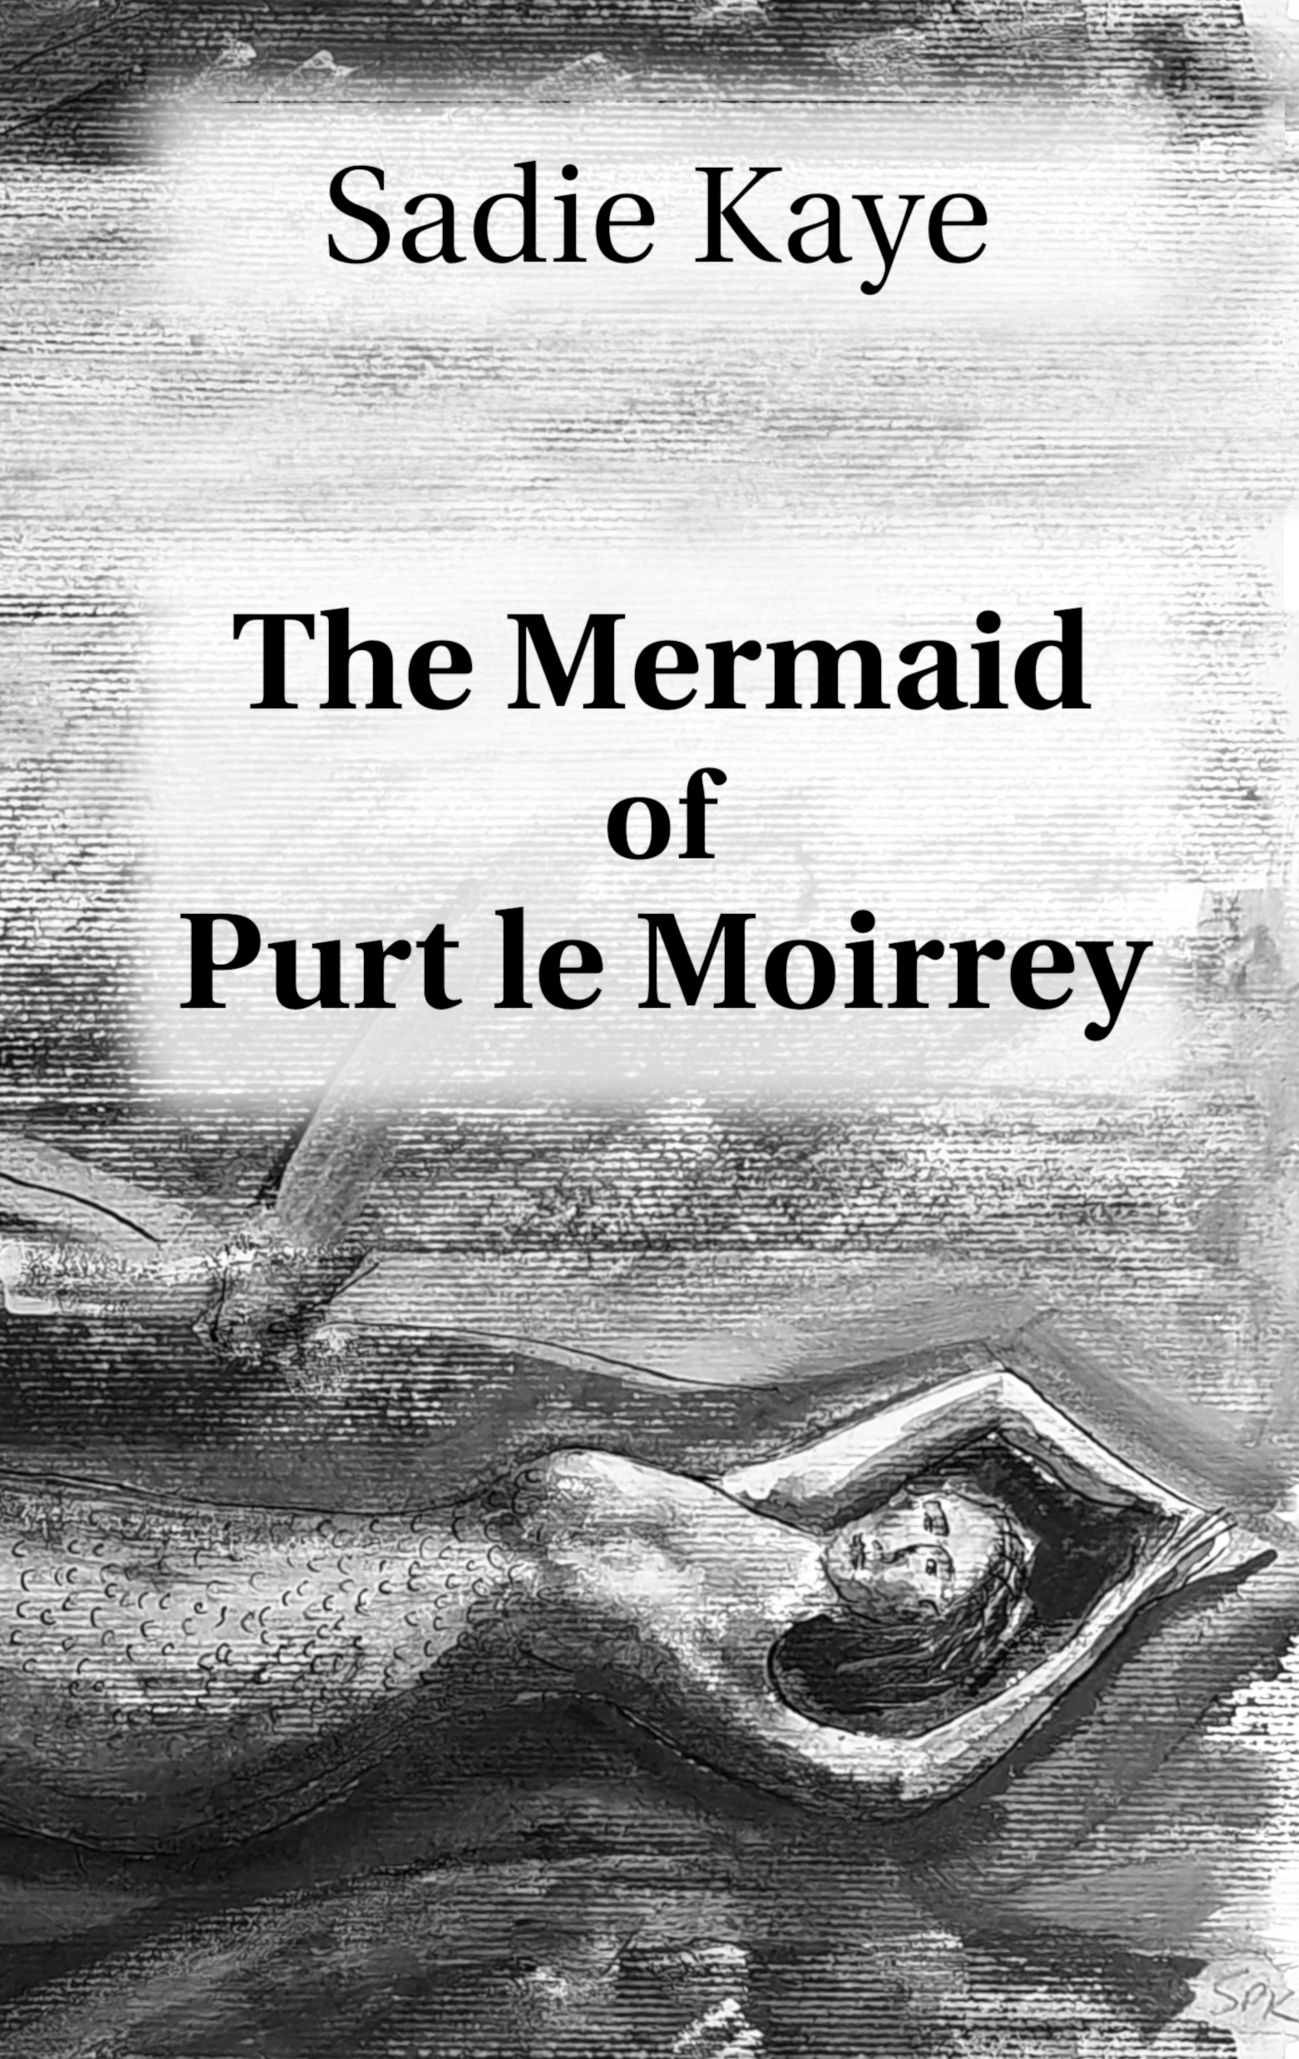
\includegraphics[width=0.58\textwidth]{mermaidcover.jpg}\hfill\parbox[b]{0.39\textwidth}{\tolerance 1000%
  %
  \textbf{The Mermaid of Purt le Moirrey,\\ by Sadie Philippa Kaye.}
  
  Samuel Collister is a poor fisherman from Purt le Moirrey (Port St Mary
  on the Isle of Man) who spots a mermaid at sea.  He follows her at sea
  and she brings him luck in his catch.  Their relationship blossoms into
  love but all is not well. Sam's mother and his fisherman friends are
  suspicious and jealous.
  
  \strut\qquad Always pointed and relevant to the modern day,
  this tale (written as a play in verse) provides a
  powerful reflection on\break
  \vskip -2.5ex%
  %
}\break
  % a
  % powerful reflection on
  love, prejudice and 
  courage to see beyond
  differences in marginalized communities.
  Paperback, 58 pages, illustrated with Sadie Kaye's pen and ink drawings.
  ISBN 978-1-914246-53-1.

  
`The Mermaid of Purt le Moirrey is a haunting and beautiful tale, part myth, part mirror, holding up the sea’s depths to our own hearts. Sadie Kaye weaves folklore into a powerful reflection on love, prejudice, and the courage to see beyond difference.' \textbf{Katie Victoria, author of: I write because\ldots}

`Updating an older fairy story put down by Dora Broome, Sadie how small-minded attitudes destroys lives and happiness.' \textbf{Jon Hartless, author of: Constructing Churchill}

  `Sadie eloquently gives a timeless myth of thwarted love modern resonance.'  \textbf{Lorna Rose, author of: Crown her with Ivy}
  
  \clearpage

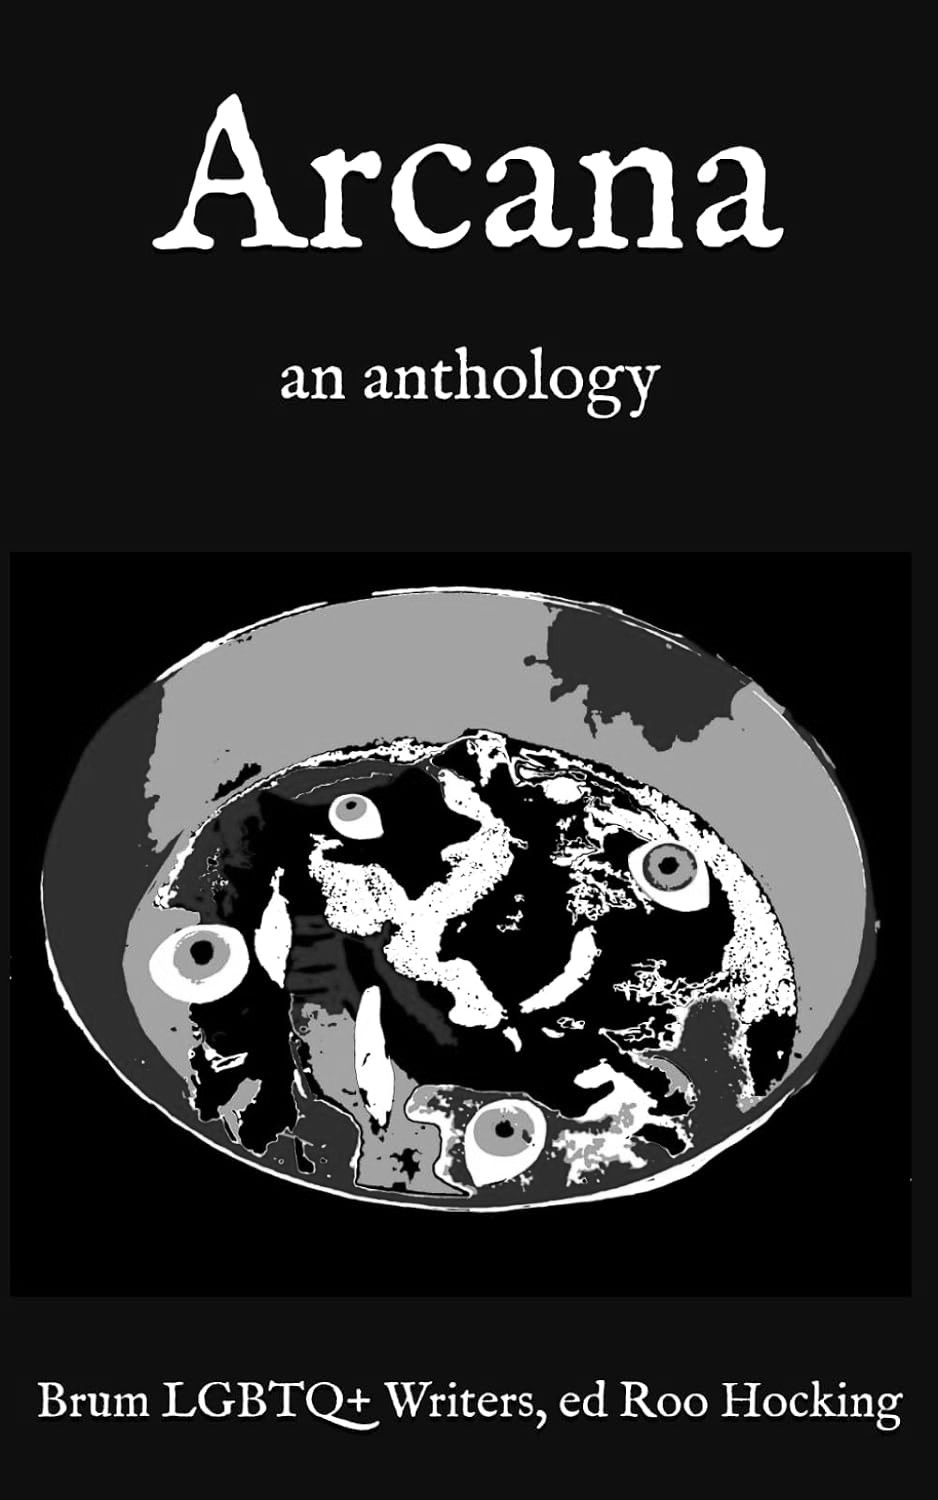
\includegraphics[width=0.48\textwidth]{arcanacover.jpg}\hfill\parbox[b]{0.49\textwidth}{\tolerance 1000%
  \textbf{Arcarna: an anthology, edited by Roo Hocking.}

  This richy illustrated anthology of new queer fiction gathers
  together twenty-two short, weird and fantastical pieces by
  Birmingham LGBTQ+ authors.  Together, they make up a new
  interpretation of the major arcana from the tarot, a curious blend
  of memory, fantasy and queer reality, with accompanying artwork by
  artist Kate Thompson.

   \strut\qquad What love story awaits the lunch-eater in the park?  Who might
   drink that Dolls Eye Soup?  And how long before her
   % dress goes up in flames?
}
dress goes up in flames?\\
  Paperback, 124 pages, ISBN 979-8319428752

  \medskip
  
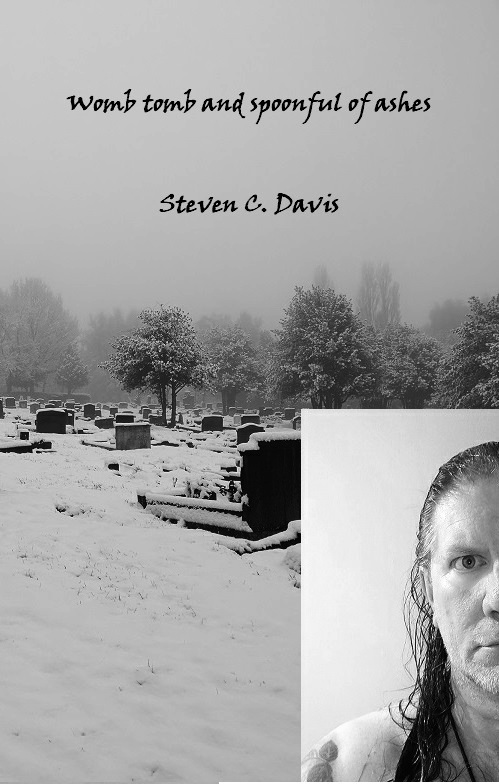
\includegraphics[width=0.48\textwidth]{wombtomb.jpg}\hfill\parbox[b]{0.49\textwidth}{\tolerance 1000%
  \textbf{Womb tomb and spoonful of ashes, by Steven C.~Davis}

A follow-up to Steven C. Davis' debut, 'Freshly dipped and bleeding
love', which was about transformation and change. This collection is
about life, death and everything in between, and quietly (and
sometimes not so quietly) rages. There are poems here about the
inequalities of the world, about being Ace, about god being a
Squirrel, about .. so much more. The underlying theme is unite. Whilst
you can achieve a lot on your own, you can achieve more
% if you join forces with others\ldots
}
if you join forces with others\ldots\\
Paperback, 68 pages, ISBN 978-1914246647 

\medskip

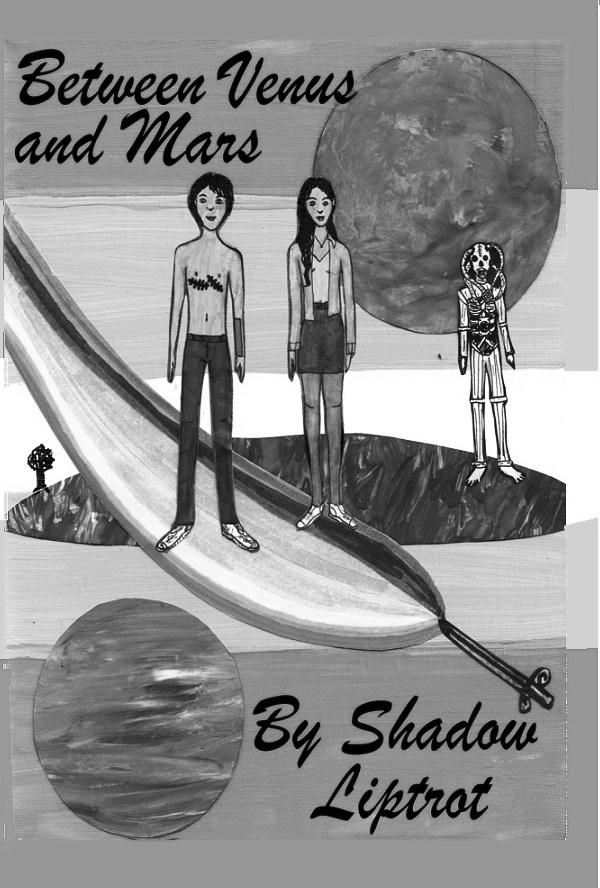
\includegraphics[width=0.48\textwidth]{VenusandMars.jpg}\hfill\parbox[b]{0.49\textwidth}{\tolerance 1000%
  \textbf{Between Venus and Mars, by Shadow Liptrot}
  
  How does it feel to be a trans man and unable to present as who you
  really are? It feels like you’re on a journey from Venus to Mars and
  you got trapped on Earth along the way. That is where Shadow
  Arlecchino is right now, except he is no longer physically on
  Earth. The president has sold humans into slavery. They have been
  put into gender camps and Shadow\=a trans man\=has been reassigned
  female.
  }
  His trauma is reawakened as he is forced to present as
  female again in order to survive. Is it worth it?

  How does it feel when the president of America sees human flesh as a
  sellable commodity? How does it feel when a writer you admired as a
  child betrays you and the entire LGBTQ+ community? How does it feel
  when aliens from the future are using AI to control everything we
  do?
  
  Paperback, 178 pages, ISBN 978-1914246630

\medskip

\medskip

\begin{center}
All available at Amazon.
\end{center}



\end{document}

